\documentclass{pfc}

%\usepackage{refcheck} % detectar figures, tablas, etc., no referenciadas

\usepackage{amsmath}
\usepackage{amssymb}
\usepackage{amsfonts}
\usepackage{mathtools}
\usepackage{pdfpages}
\usepackage{subcaption}
\usepackage{gnuplot-lua-tikz}
\usepackage{pstricks}
\usepackage{minted}
\usemintedstyle{bw}
\usepackage{listings}
\lstset{
	literate={~} {$\sim$}{1},
	language=c++,
	basicstyle=\ttfamily,
	keywordstyle=\color{blue},
	commentstyle=\color{dkgreen},
	stringstyle=\color{red},
	breaklines=true,
	breakatwhitespace=true,
	tabsize=4
}

\usepackage[noabbrev]{cleveref}

\subtitle{Informe final}

\newcommand{\TODO}[1]{{\color{red}\bfseries#1}}
\newcommand{\Nota}[1]{{\color{blue}\itshape#1}}

\newcommand{\CasoUso}[1]{\bigskip%
{\bfseries Caso de uso: #1}\par}
\newcommand{\IncCU}[1]{{\bfseries Include (#1)}}
\newcommand{\UseCU}[1]{{\bfseries Use (#1)}}
\newcommand{\CUField}[2]{{\bfseries#1:} #2\par}
\newcommand{\CUNormal}{{\bfseries Curso Normal:}\par}

\newenvironment{CasoDeUso}[1]{%
	\bigskip\begin{minipage}{.9\linewidth}
		{\bfseries Caso de uso: #1}\par
}
{%
	\end{minipage}
}


\newcommand{\Requerimiento}[2]{%
	\bigskip%
	{\bfseries #1}\\%
	#2%
}

\usepackage{algorithmicx}
\usepackage{algorithm}
\usepackage[noend]{algpseudocode}
\usepackage{booktabs}


\makeatletter
 \renewcommand{\ALG@name}{Algoritmo}
\makeatother
\renewcommand{\algorithmicfunction}{}

%\newcommand{\Alerta}[1]{{\Huge\bfseries\sffamily#1}}
\newcommand{\NombreItem}[1]{{\bfseries#1:}}

\usepackage{tikz}
\usetikzlibrary{arrows,chains,matrix,positioning,scopes}

\usepackage{environ}
\makeatletter
\newsavebox{\measure@tikzpicture}
\NewEnviron{scaletikzpicturetowidth}[1]{%
  \def\tikz@width{#1}%
  \def\tikzscale{1}\begin{lrbox}{\measure@tikzpicture}%
  \BODY
  \end{lrbox}%
  \pgfmathparse{#1/\wd\measure@tikzpicture}%
  \edef\tikzscale{\pgfmathresult}%
  \BODY
}
\makeatother

\newcommand{\bigO}{\mathcal{O}}
\newcommand{\Real}{\mathbb{R}}
\DeclareMathOperator*{\argmin}{argmin}
\DeclareMathOperator{\atan}{atan}

\graphicspath{{./uml/}{./diagram/}{./graph/}}

\newcommand{\RefImagen}[1]{ (Imagen cortesía de \cite{#1})}

\newcommand{\Em}{\hspace{1em}}

%\includeonly{reconstrucción}
\begin{document}
\frontmatter
%\TODO{revisar tiempos verbales, ahora en pasado}
	\maketitle

	\chapter{Resumen}
Gracias a los avances en sensores de profundidad y técnicas de reconstrucción de superficies,
es posible obtener con gran precisión una nube de puntos que represente
la forma, posición y dimensiones de un objeto cualquiera.
Sin embargo, esta nube de puntos es parcial, ya que solamente refleja
la porción observable desde el punto de captura.
Por esta razón, en este proyecto se propone el desarrollo de una biblioteca de software
que implemente técnicas para combinar estas vistas parciales
y así obtener un modelo tridimensional de todo el objeto,
posibilitando su posterior construcción mediante técnicas de impresión 3D.

\Nota{
	sensores de profundidad y técnicas para determinar la profundidad.

	Hablar de prime-sense, kinect fusion, que requieren que el usuario
	tome las capturas con mucho cuidado

	Nosotros hacemos pocas capturas espaciadas, esa es la gracia
%TODO: motivación continuar lo de pancho
%explayarse en la forma de adquisición
%vistas parciales
}
	%\noindent{\bfseries Palabras clave:} fusión de mallas, imágenes de profundidad, impresión 3D, reconstrucción 3D.


	\tableofcontents
	\listoffigures

\mainmatter
	\chapter{Introducción}
%zippered
%This paper presents a method of combining multiple views of an
%object, captured by a range scanner, and assembling these views into
%one unbroken polygonal surface.  Applications for such a method
%include:
%• Digitizing complex objects for animation and visual simulation.
%• Digitizing the shape of a found object such as an archaeological
%artifact for measurement and for dissemination to the scientific
%• Digitizing human external anatomy for surgical planning,
%remote consultation or the compilation of anatomical atlases.
%• Digitizing the shape of a damaged machine part to help create
%a replacement.

	\section{Justificación}
	La impresión 3D es un método de fabricación en el cual se deposita el material
	(como por ejemplo, plástico o metal) en capas para producir un objeto tridimensional.
	Avances en los materiales utilizados han permitido la creación de objetos
	de calidad comparable a la de métodos tradicionales,
	demostrando su viabilidad para muchas aplicaciones médicas,
	incluyendo la creación de prótesis e implantes dentales\cite{Schubert159}. %\cite{innovations in 3d printing}
	%con el potencial de personalizar cada producto.
	Los modelos geométricos que desean imprimirse pueden obtenerse aplicando procesos de
	reconstrucción tridimensional (figura~\ref{fig:ingenieria_inversa}) a objetos ya existentes.

	\begin{figure}
		\centering
		\begin{subfigure}{.3\linewidth}
			\Imagen{img/face-02}
			\caption{\label{fig:cara}Objeto}
		\end{subfigure}
		\begin{subfigure}{.3\linewidth}
			\Imagen{img/geometric_model}
			\caption{\label{fig:cara_3d}Modelo geométrico}
		\end{subfigure}
		\begin{subfigure}{.3\linewidth}
			\Imagen{img/print_3d}
			\caption{\label{fig:cara_print_3d}Impresión 3D}
		\end{subfigure}
		\caption{\label{fig:ingenieria_inversa}Reconstrucción tridimensional.
		A partir de un objeto (\ref{fig:cara}) se obtiene su modelo geométrico (\ref{fig:cara_3d})
		para lograr su posterior impresión 3D (\ref{fig:cara_print_3d}).}
	\end{figure}

	Entre las aplicaciones de la reconstrucción tridimensional podemos nombrar:
	\begin{itemize}
		\item Reconstrucción de órganos para la planificación de cirugías
			y la realización de prácticas por parte de estudiantes de ciencias médicas y veterinarias.
			En particular, la empresa argentina \emph{mirai}\footnote{\url{https://www.modelosmedicos.com/}} realiza estos biomodelos basándose en imágenes de resonancia magnética y tomografía computarizada.
			%mirai 3d, empresa argentina, adquiere los biomodelos mediante tomografía axial computarizada (TAC)
			\ImagenInline{img/corazon_1}
		\item Digitalización de obras de arte para salvaguardar el patrimonio cultural,
			ayudar en su restauración e incrementar la accesibilidad a las mismas.
			A este respecto, puede mencionarse el \emph{Digital Michelangelo Project} de la Universidad de Stanford, que tiene como objetivo crear un repositorio de modelos 3D de alta calidad de las esculturas y la arquitectura de Miguel Ángel.
			\ImagenInline{img/estatua_leon}
		\item Realización de prototipos y modificaciones a productos.
			\ImagenInline{img/anteojos}
		\item Simulación de propiedades físicas sobre los objetos.
			\ImagenInline{img/bunny_heat}
		\item Digitalización de ambientes y objetos para utilizarlos en aplicaciones de realidad virtual o de diseño.
			\ImagenInline{img/room}
	\end{itemize}

	Uno de los métodos para la obtención de los modelos geométricos
	se basa en la utilización de dispositivos de luz estructurada,
	como ser el dispositivo Kinect\cite{MatheEstudioKinect},
	para realizar mediciones sobre el objeto.
	Debido a que los puntos capturados sólo reflejan la porción de la superficie del objeto visible desde la cámara,
	y a que la propia geometría del objeto podría generar obstrucciones, reflejos o sombras
	que imposibilitan la adquisición de datos en esas zonas («huecos»),
	es necesario combinar múltiples capturas
	del objeto en diferentes orientaciones respecto a la cámara, de modo que
	cada parte de la superficie del objeto esté representada en al menos una captura (figura~\ref{fig:kinect_reconstruction}).

	\begin{figure}
		\Imagen{img/loop_multiple_view}
		\caption{\label{fig:kinect_reconstruction}Medición de las características geométricas de los objetos mediante múltiples capturas utilizando cámaras de profundidad.}
	\end{figure}

	%Describir los pasos de la ingeniería inversa: adquisición alineación, encuentro de superficie, descripción, segmentación, modelo CAD
	El principal problema para combinar las múltiples vistas es
	encontrar las transformaciones de rotación y translación que permitan
	relacionar cada vista parcial, para luego fusionarlas y así reconstruir el objeto.
	

	Para esto existen métodos automáticos que requieren que la posición del dispositivo de captura
	entre las distintas capturas no haya variado de forma significativa\cite{regBesl92},
	lo cual genera que el proceso de adquisición de datos sea engorroso,
	requiriendo de una supervisión constante para asegurar que el movimiento del dispositivo de captura no sea excesivo
	y donde un fallo puede exigir el reinicio del proceso.
	Este es el caso de \emph{KinectFusion}, un algoritmo desarrollado por Microsoft que utiliza el sensor Kinect para reconstruir escenas tridimensionales en tiempo real,
	pero que presenta las siguientes limitaciones:
	\begin{itemize}
		\item utiliza un alto costo computacional, requiriendo de una poderosa GPU;
		\item los movimientos de cámara deben ser lentos y pequeños;
		\item está limitado al dispositivo Kinect;
		\item algunos objetos podrían no aparecer en el mapa de profundidad debido a que absorben o reflejan demasiada luz infrarroja;
		\item no utiliza información de color.\cite{real-time-3d-reconstruction-using-a-kinect-sensor}
	\end{itemize}

	Existen, además, métodos manuales o semiautomáticos donde se permiten distancias mayores entre las posiciones del dispositivo de captura.
	Por ejemplo, el usuario posiciona de forma interactiva las capturas\cite{Turk:1994:ZPM:192161.192241}
	o selecciona iterativamente puntos coincidentes entre ellas\cite{LocalChapterEvents:ItalChap:ItalianChapConf2008:129-136}.

	Con el fin de evitar o limitar el uso de los recursos humanos,
	en este proyecto se analizarán técnicas de fusión de mallas,
	obtenidas permitiendo mayor distancia entre capturas,
	para lograr un modelo tridimensional de un objeto que permita su posterior replicación
	mediante una impresora 3D.



	\section{Objetivos}
		\subsection{General}
			Diseñar y desarrollar una biblioteca de funciones que permita
			la reconstrucción de una malla 3D cerrada a partir de mallas de superficies parciales.
		\subsection{Específicos}
		\begin{itemize}
			%Falta un objetivo específico relacionado con el análisis de técnica de fusión de mallas.
			\item Desarrollar algoritmos que determinen las posiciones relativas de cada malla parcial.
			\item Desarrollar algoritmos de fusión de las mallas.
			\item Desarrollar algoritmos para rellenado de huecos producto de obstrucciones.
			\item Evaluar el desempeño de cada bloque desarrollado y realizar ajustes.
		\end{itemize}

	\section{Alcance}
	\begin{itemize}
		\item Para posibilitar la posterior impresión 3D,
			la malla resultante deberá ser una malla cerrada (\emph{watertight}).
		\item No se impondrán topologías específicas a los objetos a reconstruir.
		\item Los algoritmos desarrollados deberán ser robustos frente al ruido producido por los sensores.
		\item No se pretenderá el funcionamiento de los algoritmos en tiempo real.
		\item La biblioteca será de código libre y multiplataforma.
	\end{itemize}

	\chapter{Reconstrucción tridimensional}

La reconstrucción tridimensional es un proceso por el cual se combinan diversas mediciones de un objeto
para obtener un modelo tridimensional que lo reproduzca fielmente.
Este proceso puede dividirse en las siguientes etapas (figura~\ref{fig:proceso_reconstruccion_3d}):
\begin{enumerate}
	\item Adquisición: en esta etapa se realizarán las mediciones del objeto,
		obteniéndose las posiciones $\{x, y, z\}$ de puntos muestreados sobre su superficie.
	\item Registración: en caso de que el método de adquisición no capture la totalidad del objeto,
		esta etapa establecerá las relaciones entre las medidas parciales
		para ajustarlas a un mismo marco de referencia.
	\item Determinación de la superficie: en esta etapa se estimará la superficie del objeto
		a partir de los puntos muestreados.
	\item Rellenado de huecos: es posible que existan zonas donde
		no se hayan obtenido muestras y, por lo tanto, la superficie presente huecos.
		Dependiendo de la aplicación, puede ser necesario rellenar estos huecos
		estimando nuevos puntos a partir de los lindantes.
		%estimando la superficie mediante los puntos lindantes.
\end{enumerate}

\begin{figure}
	\Imagen{img/reconstruccion}
	\caption{\label{fig:proceso_reconstruccion_3d}Proceso de reconstrucción.
	De izquierda a derecha y de arriba a abajo se tiene:
	objeto a reconstruir, adquisición de capturas parciales,
	registración de cada captura a un marco de referencia global,
	determinación de la superficie,
	rellenado de huecos.}
\end{figure}

A continuación se describen con más detalle estas etapas y los métodos utilizados en las mismas.

\section{Adquisición}
%Un proceso crucial en la reconstrucción tridimensional es la adquisición de datos.
Los distintos métodos de adquisición se diferencian de acuerdo al fenómeno físico de interacción
con la superficie del objeto de interés. De esta manera, se pueden clasificar como:
	\begin{itemize}
		\item Métodos táctiles o de contacto, donde sensores en las articulaciones de un brazo robótico determinan las coordenadas relativas de la superficie. Estos son de los más robustos, introduciendo poco ruido, pero también de los más lentos y suelen tener problemas con superficies cóncavas.
		\item Métodos de no-contacto, donde se utiliza luz (métodos ópticos), sonido u ondas electromagnéticas.
	\end{itemize}

En particular, los métodos ópticos son los más populares con una rápida velocidad de adquisición\cite{Várady97reverseengineering}. %\cite{reverse engineering}.
Dentro de los métodos ópticos podemos distinguir:
\begin{itemize}
	\item Métodos pasivos o de visión estereoscópica,
		que utilizan dos o más cámaras y buscan correspondencias
		entre los puntos de la escena capturados en cada fotografía.
	\item Métodos activos o de luz estructurada,
		que proyectan patrones de luces conocidos sobre la escena de modo de analizar sus deformaciones.
\end{itemize}
Identificar los patrones lumínicos es un problema más simple que el de
encontrar las correspondencias entre imágenes, por lo que los métodos de luz
estructuradas resultan más rápidos y robustos\cite{Pancho}.

%FIXME
%volarlo todo y decir que los métodos ópticos me dan una nube de puntos 2.5D,
%orientada en el sistema de referencia de la cámara
A partir de los métodos ópticos se obtendrá como resultado una imagen de profundidad, donde el valor de
cada píxel representa la distancia entre el punto observado y la cámara, lo cual se conoce como imagen 2.5D.
Conociendo los parámetros intrínsecos $K$ de la cámara,
puede obtenerse para cada píxel $\{X, Y, d\}$ sus coordenadas $\{x, y, z\}$ en el espacio:
\[
	\left(\begin{matrix}
		x \\ y \\ z \\
	\end{matrix}\right) =
	K^{-1}
	\left(\begin{matrix}
		X \\ Y \\ d \\
	\end{matrix}\right)
\]
Estas son coordenadas locales, definidas en un sistema de referencia centrado en la cámara.


Se tendrá entonces una \emph{nube de puntos}, es decir, una colección de puntos
sin información de conectividad entre ellos.
%Se observa, además, que no existen dos puntos con las mismas coordenadas $\{x, y\}$, es decir, la nube de puntos es 2.5D.
Esta nube de puntos será una representación parcial de la superficie del objeto,
ya que se corresponderá únicamente con la porción observable desde la cámara.


Si bien este proyecto no abarca la etapa de adquisición,
no es posible ignorar el método de adquisición,
ya que este influye en las características de la nube de puntos resultante.
Por esta razón, se supondrá que las capturas provienen de métodos ópticos de luz estructurada.


\subsection{Ruido de adquisición}
Es imposible obtener la posición exacta de los puntos muestreados sobre la superficie del objeto.
%FIXME: si alguien tiene ganas de ayudar
Se tendrán distorsiones debidas a particularidades de la escena, del objeto, de los
dispositivos utilizados y del método empleado.
En los escáneres de luz estructurada dos fuentes de error son particularmente relevantes:
\begin{itemize}
	\item \emph{Ángulo de incidencia excesivo:}
		El rayo de luz proyectado impacta en una porción de la superficie del objeto
		que es casi paralela a su dirección.
		Entonces, el sensor capta
		una versión estirada y con menor intensidad del patrón, %(figura~\ref{fig:error_distorsion}),
		lo que agrega incertidumbre en la posición de los puntos.
	\item \emph{Reflejo parcial:}
		Se produce cuando una porción del patrón no incide completamente en el objeto (figura~\ref{fig:error_adquisicion}).
		Debido a que el método de triangulación supone que todo el ancho de la línea impactó en el objeto,
		se estima una posición incorrecta del punto muestreado.
		Esto resulta en bordes distorsionados y en posiciones más alejadas que las reales.\cite{Turk:1994:ZPM:192161.192241}
\end{itemize}

%\begin{figure}
%	\Imagen{foo}
%	\caption{\label{fig:error_distorsion}El patrón a identificar se encuentra estirado debido a que los haces de luz inciden con un ángulo excesivo sobre la superficie.}
%\end{figure}
\begin{figure}
		\Imagen{diagram/error_adquisicion_borde}
		\caption[Error debido a un reflejo parcial]{\label{fig:error_adquisicion}Error en la posición estimada debido a un reflejo parcial del patrón de luz.}
\end{figure}

\endinput

\section{Registración}
Una vez finalizada la etapa de adquisición, se dispone de una nube de puntos
que representa la porción observada del objeto.
Para lograr una reconstrucción total es necesario combinar múltiples capturas
variando la posición relativa cámara-objeto.
Contar con un dispositivo que nos permita definir con precisión
tanto la posición como orientación de la cámara es altamente costoso,
por esta razón, en la etapa de registración se deben estimar las transformaciones que ubiquen cada
captura en un sistema de referencia global, de forma que las zonas comunes encajen perfectamente.


Esta operación se realiza usualmente entre dos capturas,
buscando las transformaciones de translación y rotación que ubiquen
la captura de partida en el marco de referencia de la captura objetivo.
De esta manera, el problema general cuenta con seis grados de libertad.
A continuación se presenta el caso en que
la transformación de alineación es pequeña,
más adelante se discute el caso de incrementos mayores,
y finalmente se extiende el proceso para abarcar $n$ capturas.

%esto va en $N$ capturas
%Para extender este proceso a $n$ capturas, puede alinearse $C_0$ con $C_1$,
%$C_1$ con $C_2$, $C_2$ con $C_3$, etc.,
%sin embargo, el error de registración se propagará en cada paso.


\subsection{Perturbaciones pequeñas: algoritmo iterativo del punto más cercano (ICP)}
Antes de describir este algoritmo, se planteará una versión simplificada del problema
que permitirá establecer ciertas definiciones.

Se supone que se dispone de una nube $A$ a la cual se le aplica
una transformación de translación y rotación arbitraria,
y luego se perturba levemente
las posiciones de los puntos transformados,
obteniéndose la nube $B$.
Se observa que ambas nubes poseen la misma cardinalidad y se pueden establecer las relaciones de origen a destino
$a_j \to b_j$ para cada punto $a_j \in A$.
Entonces, se puede definir el error de alineación como:
\[
	\text{Error} = \frac{1}{N} \sum_{j=1}^n || b_j - T \left(a_j\right) ||
\]
y buscar la transformación $T$ que minimice este error.

Existe una solución cerrada para este problema, obteniéndose la rotación al
calcular los eigenvectores de una matriz simétrica de $4\times4$,
cuyos detalles pueden consultarse en \cite{Horn87closed-formsolution}.

Sin embargo, estas suposiciones son demasiado fuertes.
Al trabajar con dos capturas realizadas desde distintas vistas, el solapamiento no será total,
ya que habrá puntos que serán observables en tan sólo una de las vistas.
Por lo tanto, primero es necesario determinar cuáles son los puntos comunes a ambas capturas,
y, además, definir las relaciones de origen-destino entre esos puntos comunes.
El algoritmo iterativo del punto más cercano (ICP) supone que las nubes se encuentran
lo suficientemente cerca como para establecer estas correspondencias mediante las coordenadas de los puntos.
El algoritmo se describe de la siguiente manera:
\begin{enumerate}
	\item Obtener las correspondencias:
		Para cada punto $a_j \in A$ buscar el punto más cercano en la nube $B$.
		Si la distancia entre esos puntos supera un umbral $d_{\text{max}}$,
		se considera que $a_j$ no pertenece a la zona común y no es considerado en esta iteración.
	\item Calcular la transformación que alinee los pares de puntos de la zona común.
	\item Aplicar la transformación.
	\item Repetir el proceso hasta que el error de alineación esté por debajo de un umbral $\tau$.
\end{enumerate}%\cite{conf/rss/SegalHT09}
Si bien el algoritmo converge a un mínimo local, puede que este no sea el mínimo global buscado.
Debe cumplirse la suposición de cercanía para obtener una correcta registración.\cite{regBesl92}

%generalized conf/rss/SegalHT09
En \cite{chen-medoni} se presenta una variante del algoritmo de ICP, llamada ICP {punto-a-plano},
que resulta más robusta y precisa al trabajar con nubes de puntos en 2.5D.
Una vez establecida una correspondencia $a_j \to b_j$, si bien no se trata del mismo punto,
se realiza la suposición de que pertenecen al mismo plano.
Por esta razón, podemos decir que conocemos con mucha confianza la posición del punto
a lo largo de su normal, pero no su ubicación en el plano.
Para reflejar esto, se cambia la métrica del error, proyectando el punto transformado sobre la normal
del punto destino (figura~\ref{fig:point_to_plane}).
\[
	\text{Error} = \frac{1}{N} \sum_{j=1}^n || n_j \cdot \left( b_j - T \left(a_j\right) \right) ||
\]

\begin{figure}
	\centering
	\input{diagram/icp_point_to_plane.pdf_tex}
	\caption[Medidas de error punto-a-plano entre dos superficies]{\label{fig:point_to_plane}Medidas de error punto-a-plano entre dos superficies
	(Imagen cortesía de \cite{icp_point_to_plane}).}
\end{figure}


\subsection{Distancias mayores: búsqueda de correspondencias mediante vectores de características}
Cuando la transformación de alineación requerida para alinear las dos nubes de puntos
no es lo suficientemente pequeña, no se obtiene una buena aproximación al establecer las correspondencias
utilizando únicamente las posiciones de los puntos.
Una posibilidad es emplear métodos semiautomáticos, donde el usuario provee de una alineación inicial
de las nubes o determina las correspondencias seleccionando puntos.
Sin embargo, este es un método lento y engorroso,
por lo que surge la necesidad de plantear un algoritmo completamente automático.

Para hallar las correspondencias de manera automática, se calcula un vector de características o \emph{descriptor}
sobre una vecindad de cada punto. Al comparar los descriptores con alguna medida de distancia,
si la distancia es pequeña (cercana a $0$), entonces las vecindades son similares
y podría plantearse una correspondencia entre los puntos.
Un buen descriptor deberá poseer las siguientes características:
\begin{itemize}
	\item Ser discriminante, es decir, la distancia entre los descriptores debe reflejar
		la distancia entre las superficies de las vecindades.
		Esto implica que superficies similares localmente producen descriptores parecidos, y
		en superficies diferentes la distancia entre descriptores será grande (figura~\ref{fig:descriptor_matriz_confusion}).
	\item Ser invariante respecto a translaciones y rotaciones.
	\item Ser robusto respecto al ruido de muestreo.
	\item Ser robusto respecto a la densidad de muestreo.
	\item Ser robusto respecto a la ausencia de muestras debido a oclusiones.
\end{itemize}

\begin{figure}
	\centering
	\input{diagram/fpfh_confusion.pdf_tex}
	\caption[Matriz de confusión del descriptor FPFH]{\label{fig:descriptor_matriz_confusion}Matriz de confusión del descriptor FPFH para distintas clases de superficies utilizando la distancia $\chi^2$\RefImagen{RusuDoctoralDissertation}.}
\end{figure}

Además de la elección del descriptor, un parámetro importante a determinar es
el tamaño de la vecindad que éste representará.
En general, la vecindad de un punto $p$ incluye a todos aquellos puntos $q$
que se encuentran dentro de una esfera de radio $r$ centrada en $p$:
\[ |p - q| \leq r \]
Si el valor de $r$ es demasiado pequeño, el descriptor perderá su poder discriminante
o incluso no podrá calcularse al no contar con la cantidad de vecinos mínimos necesarios.
% FIXME:
%sobrecarga significado «superficie»
%el riesgo al incrementar la vecindad es que sea «otra cara» de la superficie
%no sé, hablar de continuidad o de localidad
En cambio, si el valor de $r$ es demasiado grande, se corre el riesgo de considerar
dentro de la vecindad puntos pertenecientes a otra superficie, distorsionando el valor del descriptor.
La determinación de un valor adecuado de $r$ limita la posibilidad de obtener un método completamente
automático para el cálculo de los descriptores\cite{RusuDoctoralDissertation}.
 %This issue is of extreme importance and constitutes a limiting factor in the automatic estimation (i.e., without user given thresholds) of a point feature representation.


A continuación se describe el proceso de construcción de dos descriptores
que han mostrado buenos resultados en problemas de registración\cite{Rusu:2009:FPF:1703435.1703733}.

\subsubsection{Estimación de normales}
Para poder describir la geometría de una superficie,
primero debe estimarse su orientación en el sistema de coordenadas, es decir, estimar su normal.
Una opción es aproximar la normal mediante la estimación de un plano tangente a la superficie,
lo que transforma el problema en ajustar un plano a la vecindad de $p$
mediante el método de mínimos cuadrados.
Representando el plano mediante un punto $x_j$ y un vector normal $n_j$,
la distancia de un punto $q$ de la vecindad a este plano queda definida como
$d = (q_j - x_j) n_j$.
Para minimizar la sumatoria del cuadrado de todas las distancias, se tiene que:
\[x_j = \frac{1}{N} \sum_{k=1}^{N} q^{(k)}_j \]
para los $N$ puntos de la vecindad de $p$.
Y para obtener $n_j$ se analizan los eigenvalores y eigenvectores de la matriz de covarianza de la vecindad:
\[ C_{jk} = \sum_{r=1}{N} (q^{(r)}_j - x_j) (q^{(r)}_k - x_k) \]

Se observa que $C_{jk}$ es una matriz simétrica y por lo tanto todos sus eigenvalores son reales
$\lambda_j \in \Real$.
El eigenvector que corresponde al eigenvalor de menor magnitud corresponde a la normal del plano tangente,
es decir a $+n_j$ o a $-n_j$\cite{10.1109/34.334391}.
Si bien no puede determinarse matemáticamente el signo de $n_j$,
puede resolverse la ambigüedad al considerar que la nube de puntos que se obtiene del proceso de adquisición
es 2.5D y se conoce la ubicación de la cámara $v_j$ en un sistema de referencia local.
Por lo tanto, debe cumplirse que:
\[n_j v_j > 1\]
invirtiendo el signo de $n_j$ en caso de ser necesario.

\subsubsection{Histograma de características del punto (PFH)}
Dado que las normales no son invariantes a rotaciones y no capturan mucho
detalle de la superficie, no presentan un gran poder discriminante.
Por esta razón, no resulta adecuado utilizarlas como único descriptor.
Sin embargo, al representar las relaciones entre todos los puntos de la vecindad y sus normales,
pueden capturarse con más detalle las variaciones de la superficie,
aumentando la representatividad del descriptor.
Esta es la idea principal del histograma de características del punto (PFH) presentado en \cite{RusuDoctoralDissertation}.

El vector de características de PFH es un histograma de los valores de tres ángulos
y una distancia calculados para cada par de puntos y sus normales en la vecindad de $p$.
Para asegurar la replicabilidad del descriptor, se define un marco de referencia de Darboux
%FIXME: dónde poner la referencia
(figura~\ref{fig:pfh_marco_referencia})
determinado unívocamente de la siguiente manera:
\begin{itemize}
	\item Dado el par de puntos $p_j$ y $p_k$, se determina el origen $p_s$ del marco de referencia como:
		\[
			\vec{n}_j \cdot (p_k - p_j) > \vec{n}_k \cdot (p_j - p_k)
			\begin{cases}
				\text{Verdadero: }& p_s = p_j \quad p_t = p_k\\
				\text{Falso: }& p_s = p_k \quad p_t = p_j\\
			\end{cases}
		\]
	\item A partir de este origen, se determinan los tres vectores que definen el marco de referencia:
\[
	\begin{cases}
		u =& n_s \\
		v =& u \times \displaystyle\frac{p_t - p_s}{|p_t - p_s|} \\
		w =& u \times v \\
	\end{cases}
\]
\end{itemize}
Y entonces se procede a calcular las siguientes relaciones para estos puntos:
	\begin{align*}
		d        &= |p_t - p_s| \\
		\alpha   &= v \cdot n_t \\
		\phi     &= u \cdot \frac{p_t - p_s}{d}\\
		\theta   &= \atan(w \cdot n_t, u \cdot n_t)
	\end{align*}
Sin embargo, la distancia entre puntos $d$ no es de importancia para escaneos 2.5D,
ya que la distancia entre vecinos se incrementa con la distancia a la cámara,
y suele ser beneficioso omitirla en estos casos \cite{RusuDoctoralDissertation}.

%propio
Para entender el poder discriminante del descriptor PFH, es preciso comprender el significado
de los ángulos calculados entre los pares de puntos (ver figura~\ref{fig:pfh_angulos}).
Considerando el plano tangente a $p_s$, el ángulo $\phi$ mide la separación de la posición de $p_t$ respecto a este plano.
Luego, considerando el plano $wu$, donde se encuentran $p_s$, $p_t$ y $n_s$, y cuya normal es $v$:
\begin{itemize}
	\item el ángulo $\alpha$ mide el desvío de la normal $n_t$ respecto a este plano,
	\item el ángulo $\theta$ mide la distancia entre las proyecciones de las normales sobre este plano.
\end{itemize}
De esta manera, se logra describir con buen detalle las características de la superficie en la vecindad de cada punto.



\begin{figure}
	\centering
	\input{diagram/marco_ref_fpfh.pdf_tex}
	\caption[Representación gráfica del marco de Darboux]{\label{fig:pfh_marco_referencia}Representación gráfica del marco de Darboux y las características calculadas por el descriptor PFH \RefImagen{RusuDoctoralDissertation}.}
\end{figure}

\begin{figure}
	\centering
	\input{diagram/fpfh_meaning.pdf_tex}
	\caption[Representación gráfica de los ángulos $\phi$ y $\theta$ calculados por el descriptor PFH]{\label{fig:pfh_angulos}Representación gráfica de los ángulos $\phi$ y $\theta$ calculados por el descriptor PFH.}
\end{figure}

\subsubsection{PFH rápido (FPFH)}
Debido a que para obtener el descriptor PFH de un punto es necesario calcular
las relaciones entre todos los pares de puntos de su vecindad,
el orden de ejecución para una nube con $n$ puntos es $\bigO(nk^2)$,
donde $k$ es la cantidad de puntos en la vecindad,
y por esta razón el cálculo de este descriptor puede convertirse
en uno de los cuellos de botella del proceso.

Para solventar este problema, en \cite{Rusu:2009:FPF:1703435.1703733} se propone
una simplificación del descriptor PFH, llamada PFH rápido o simplemente FPFH,
que nos permite reducir el tiempo de ejecución a $\bigO(nk)$
manteniendo el poder descriptivo de PFH.

El cálculo de este nuevo descriptor se realiza de la siguiente manera:
\begin{enumerate}
	\item Calcular por cada punto $p$ y sus vecinos las tuplas $\langle \alpha, \phi, \theta \rangle$.
		Llamamos a estas características PFH simplificado (SPFH).
	\item Realizar un promedio ponderado de los valores del SPFH de $p$ y sus vecinos:
		\[
			FPFH(p) = SPFH(p) + \frac{1}{N} \sum_{j=1}^{N} \frac{1}{w_j} SPFH(p_j)
		\]
		donde $w_j$ es una medida de distancia entre $p$ y su vecino.
\end{enumerate}
%FIXME: fpfh para un punto toma sus vecinos, pfh coma todos los pares
% no quedó bien explicado
Las principales diferencias respecto a PFH son:
\begin{itemize}
	\item FPFH no interconecta todos los vecinos de $p$.
	\item FPFH puede incluir puntos fuera del radio $r$ de vecindad, pero a no más de $2r$.
\end{itemize}


\subsubsection{Puntos salientes (\emph{keypoints})}
Al describir las características de un buen descriptor, mencionamos la capacidad discriminante del mismo.
Se presenta una gran diferencia entre descriptores de superficies diferentes,
pero la distancia es cercana a $0$ en superficies parecidas,
y de esta forma se pueden establecer las correspondencias entre los puntos de dos nubes
al comparar sus descriptores.

Al analizar una zona homogénea en una nube, como, por ejemplo, un plano,
todos los puntos presentarán descriptores parecidos.
Surgen problemas al intentar establecer una correspondencia entre estos puntos
y los presentes en la otra nube, ya que todos son candidatos igualmente válidos.

Para solucionar este problema, es necesario identificar puntos salientes (\emph{keypoints})
en la nube, para entonces establecer las correspondencias entre los descriptores de estos keypoints.
Si bien un punto cualquiera será considerado como saliente o no dependiendo del detector utilizado,
un buen detector presentará las siguientes características:
\begin{itemize}
	\item Dispersión: un subconjunto pequeño de los puntos de la nube serán considerados como keypoints.
	\item Repetibilidad: un keypoint deberá ser detectado en la misma ubicación
		sobre el objeto sin importar la posición de la cámara al realizar la captura.
	\item Distinguibilidad: la superficie en la vecindad del keypoint
		presentará características únicas que serán capturadas por un descriptor.
\end{itemize}

Como ejemplos de detectores se puede mencionar el detector de esquinas Harris,
utilizado usualmente en imágenes 2D, adaptado al espacio tridimensional
traduciendo cambios en la intensidad de píxeles por ángulos entre las normales de puntos vecinos;
y el detector ISS, que analiza los eigenvalores de la matriz de covarianza en la vecindad de un punto.


\subsection{Registración de múltiples capturas}
Previamente se describieron métodos de registración entre dos capturas,
sin embargo, un objeto difícilmente pueda ser observable completamente desde tan sólo dos posiciones.
Por lo tanto, para lograr la reconstrucción tridimensional se tendrá una lista de capturas
${A_1, A_2, \ldots, A_n}$ correspondientes a distintas posiciones relativas cámara-objeto.
Surge entonces el problema de cómo obtener la lista de transformaciones ${T_1, T_2, \ldots, T_n}$
que las alinee a todas correctamente.

Una opción es utilizar una captura $B$ que presente zonas comunes con todas las capturas $A_j$
y entonces calcular la registración $A_j \to B$.
Esta captura $B$ puede obtenerse mediante un escaneo cilíndrico: el objeto se
ubica sobre una superficie que gira lentamente a una velocidad controlada
mientras que se proyecta una línea vertical sobre el objeto y se miden las
distancias de los puntos que caen sobre esta línea.

Una alternativa es realizar la registración entre pares sucesivos
$A_2 \to A_1$,
$A_3 \to A_2$,
\ldots,
$A_{n} \to A_{n-1}$.
Sin embargo, los errores producidos se propagarán con cada
captura incorporada, siendo especialmente apreciables al completar una
vuelta alrededor del objeto (figura~\ref{fig:error_bucle}).
Para corregir este error, se ajustará la alineación de la captura que cierre el bucle,
propagando luego esta corrección a las demás.


	\begin{figure}
		\Imagen{diagram/error_bucle_inhand}
		\caption[Visualización del error de bucle]{\label{fig:error_bucle}Visualización del error de bucle. Errores de tan sólo $1^{\circ}$
		en cada registración producen una discrepancia considerable
		donde el modelo debería cerrarse (círculo rojo) \RefImagen{5457479}.}
	\end{figure}

\section{Módulo de fusión}
	%¿citas?
	%en el de loop correction (surfel)
	El módulo de fusión tiene como objetivo obtener un modelo que
	describa la geometría del objeto escaneado.
	Para esto, el modelo se inicializa a partir de una captura cualquiera
	y se procesan una a una las capturas correspondientes a las otras vistas.
	En cada nueva vista se agrega información del objeto en zonas que no eran antes visibles
	y además se confirma o refuta la información ya presente en el modelo.
	Al combinar esta información, el módulo de fusión obtiene finalmente una malla
	que represente a la totalidad del objeto.

	\subsection{Método}
	Se utiliza una representación de \emph{surfel} para cada punto similar a la propuesta en \cite{5457479} %ref in-hand scanning
	debido a la facilidad de implementación de las funciones de actualización de los puntos.
	Como es necesario integrar la información de posición y normal de cada punto,
	se idearon funciones de conversión del formato de nube usado en el módulo de registración.

	Cada surfel tiene asociado un valor de confianza y las vistas en las que
	fue observado.  El valor de confianza nos indica la probabilidad de que sus
	valores de posición y normal no sean producto de un error de muestreo.
	Este valor se inicializa según el ángulo de su normal respecto a la línea
	de la cámara (figura~\ref{fig:confianza_surfel}).
	%y a su distancia al centro de la captura %terminé usando sólo las normales

	\begin{figure}
		\Imagen{img/bunny_confianza}
		\caption[Visualización de los valores de confianza de los súrfeles]{\label{fig:confianza_surfel}Visualización de los valores de confianza de los súrfeles para la captura \texttt{bun000}.}
	\end{figure}

	El algoritmo~\ref{alg:surfel} describe el agregado de una nueva vista.
	Por cada punto de la vista se busca qué surfel lo contiene y se actualiza
	su posición y normal ponderando según el nivel de confianza.
	\begin{eqnarray*}
		\hat{P}_k = \frac{\sum_{j} \alpha_j P^{(j)}_k}{\sum_{j} \alpha_j} \\
		\hat{n}_k = \frac{\sum_{j} \alpha_j n^{(j)}_k}{\sum_{j} \alpha_j}
	\end{eqnarray*}
	En caso de que haya caído fuera del dominio de la reconstrucción actual, se
	considera que es un nuevo punto y se lo agrega.
	Si la distancia de proximidad elegida es demasiado pequeña,
	nunca se realizará la actualización ya que todos los puntos serán considerados como nuevos surfels.
	En cambio, si la distancia es muy grande, se considerarán puntos
	que deberían haber sido descartados como atípicos.

	\begin{algorithm}
		\begin{algorithmic}[1]
			\Function{Agregar vista}{vista, reconstrucción}
				\ForAll{$p \in \mbox{vista.puntos}$}
					\State surfel $\gets$ reconstrucción.buscar(p)
					\If {surfel = $\emptyset$}
						\State reconstrucción.agregar(p)
					\Else
						\State surfel.actualizar(p)
					\EndIf
				\EndFor
			\EndFunction
		\end{algorithmic}
		\caption[Actualización de la reconstrucción al agregar una nueva vista]{\label{alg:surfel}Actualización de la reconstrucción al agregar una nueva vista.}
	\end{algorithm}

	Al terminar de procesar todas las vistas, habrá surfels que hayan sido
	observados desde sólo una posición y tengan un nivel de confianza bajo.
	Estos son considerados como ruido y eliminados de la
	reconstrucción.

	Finalmente, se procede a la obtención de una triangulación de los surfels.
	Para esto se empleó el algoritmo de \emph{Greedy Projection Triangulation} que provee PCL,
	el cual realiza una proyección de la vecindad de un punto en el plano definido por su normal
	y procede a conectar los puntos de modo que los triángulos resultantes
	respeten umbrales de longitud y ángulos definidos por el usuario (figura~\ref{fig:surface}).

	\begin{figure}
		\Imagen{img/bun_fusion}

		%\Imagen{img/bun_fusion_conf}
		\caption[Superficie reconstruida]{\label{fig:surface}Superficie reconstruida. En verde se destacan los bordes de los huecos.}
	\end{figure}

\section{Módulo de rellenado de huecos}
	Al finalizar el algoritmo de fusión se obtuvo una malla triangular a partir
	de la información proveniente de cada vista.
	Sin embargo, esta malla no es cerrada ya que existen zonas que ninguna
	vista pudo capturar y por lo tanto carecen de puntos, produciendo huecos en la misma.

	El módulo de rellenado de huecos se encargará de estimar, de forma automática, la superficie del
	objeto en estas zonas para así obtener finalmente una malla cerrada.

	Se plantearon dos métodos:
	\begin{itemize}
		\item \emph{Advancing front}, que trabaja localmente con los puntos que forman el contorno de cada hueco.
		\item Reconstrucción de Poisson, que trabaja con todos los puntos de la nube a la vez. 
	\end{itemize}


	\subsection{Advancing front}
		En este método, cada hueco se rellenará de forma independiente a los otros,
		utilizando únicamente los puntos que conforman cada contorno para estimar
		las posiciones de los nuevos puntos.
		Tomando en cuenta esas consideraciones, se diseñó el diagrama de clases presentado en la figura~\ref{fig:filling_class},
		cuyas clases principales se describen a continuación:
		\begin{itemize}
			\item {\bfseries Relleno de huecos:} La clase se encarga de estimar
				nuevos puntos en zonas donde se carece de información (huecos)
				y triangularlos para que la \emph{Malla} sea cerrada.
			\item {\bfseries Borde:} Es una colección de puntos ordenados
				que representa un borde de un hueco en la \emph{Malla}.
		\end{itemize}

		\begin{figure}
			\Imagen{uml/hole_filling}
			\caption{\label{fig:filling_class}Diagrama de clases del módulo de registración}
		\end{figure}

		Es posible que dentro de un hueco se observen puntos que no lograron
		conectarse al resto de la malla.  Si bien estas islas nos brindan
		información de la superficie, su presencia dificulta la identificación
		del contorno de cada hueco.  Por esta razón, se eliminaron todas las
		islas al trabajar únicamente con la componente conectada que contenía
		la mayor cantidad de puntos.
		De esta forma, una arista que defina sólo un triángulo formará parte de un hueco,
		y podrá obtenerse el contorno del mismo recorriendo el grafo de conectividades. 

		\TODO{gráficos}
		El rellenado se implementó mediante una variante del método de
		\emph{advancing front}\cite{advance_front}, descripta en el
		algoritmo~\ref{alg:adv_front}.

		Los nuevos puntos insertados son elegidos de forma que los triángulos resultantes sean
		aproximadamente equiláteros, como se detalla en el algoritmo~\ref{alg:new_point}.
		Estos puntos son luego proyectados en un plano de soporte definido
		mediante las normales de los puntos del ángulo candidato.

		En caso de que el nuevo punto cayese cerca de otro ya existente, se utilizará aquel.
		Esto implica dividir en dos el hueco, y cada nueva porción se rellenará de forma independiente.
		\TODO{gráfico}

		\begin{algorithm}
			\begin{algorithmic}[1]
				\Function{Advancing front}{Malla, Contorno}
					\State AF $\gets$ Contorno
					\Repeat
					\State $\alpha = \widehat{PCN} =$ ángulo mínimo(Contorno)
					\If{$\alpha < 75^{\circ}$}
						\State Malla.agregar triángulo(P, C, N)
						\State AF.eliminar punto(C)
					\ElsIf{$\alpha < 135^{\circ}$}
						\State nuevo $\gets$ crear punto(P, C, N, $\alpha/2$)
						\State Malla.agregar punto(nuevo)
						\State Malla.agregar triángulo(nuevo, C, N)
						\State AF.insertar punto(nuevo)
					\ElsIf{$\alpha < 180^{\circ}$}
						\State nuevo $\gets$ crear punto(P, C, N, $\alpha/3$)
						\State Malla.agregar punto(nuevo)
						\State Malla.agregar triángulo(nuevo, C, N)
						\State AF.insertar punto(nuevo)
					\EndIf
					\Until $\mbox{AF} \neq \emptyset$
				\EndFunction
			\end{algorithmic}
			\caption{\label{alg:adv_front}Relleno de huecos mediante el método de \emph{advancing front}.
			Los umbrales fueron elegidos de forma de obtener triángulos con ángulos cercanos a $60^{\circ}$.}
		\end{algorithm}

		\begin{algorithm}
			\begin{algorithmic}[1]
				\Function{crear punto}{P, C, N, $\theta$}
					\State planoA $\gets$ plano(P, C, N)
					\State planoB $\gets \left\{
						\begin{tabular}{l}
							.punto $\gets$ promedio(P, C, N) \\
							.normal $\gets$ promedio(P.normal, C.normal, N.normal)
						\end{tabular}
						\right.$
					\State Q $\gets$ rotar(
						punto = N,
						origen = C,
						\Statex normal = planoA.normal,
						ángulo = $\theta$
						)
					\State \Return proyección(Q, planoB)
				\EndFunction
			\end{algorithmic}
			\caption{\label{alg:new_point}Creación del nuevo punto}
		\end{algorithm}

		Con este método se pueden rellenar agujeros pequeños, obteniéndose una malla bastante regular (figura~\ref{fig:fill_good}).
		Sin embargo, debido a la localidad con la que se generan los nuevos
		puntos, el frente puede diverger o pretender unirse a puntos que no
		forman parte del contorno del hueco, resultando una malla mal formada,
		con aristas que corresponden a más de dos caras (figura~\ref{fig:fill_bad}).
		Para evitar la divergencia es necesario definir una superficie de
		soporte considerando todo el contorno del hueco, de forma de asegurar
		que los nuevos puntos no excedan los límites del hueco.

	\begin{figure}
		\Imagen{img/fill_good}
		\caption{\label{fig:fill_good}Relleno de un hueco pequeño mediante \emph{advancing front}.}
	\end{figure}

	\begin{figure}
		\Imagen{img/fill_bad}
		\caption{\label{fig:fill_bad}Fallo en el algoritmo de \emph{advancing front}. Se intentó completar un triángulo con un punto que no pertenecía al borde.}
		\TODO{cambiar gráfico}
	\end{figure}

	\subsection{Reconstrucción de Poisson}
	%Poisson
	La clase pcl::Poisson provee algoritmos de reconstrucción basados en \cite{Kazhdan:2006:PSR:1281957.1281965}, %cite Poisson surface reconstruction
	siendo el principal parámetro la profundidad del octree utilizado,
	impactando directamente en la resolución de la malla resultante.


	Entonces, se convierte el problema en la resolución de una ecuación de Poisson de la forma:
	\[\Delta\chi \equiv \nabla \cdot\nabla\chi = \nabla \vec{n}\]

	Se realiza una discretización del dominio mediante un octree, ya que sólo
	interesa la solución de la función en la proximidad de la superficie a
	reconstruir.
	Luego se definen funciones de soporte local que aproximen una gaussiana.

	Una vez resuelto el problema en el dominio, se extrae la isosuperficie mediante una variante del método de marching cubes.

	La malla resultante presenta un hueco en la base (figura~\ref{fig:fill_poisson}).
	Ya que los puntos del contorno del hueco pertenecen a un mismo plano, es posible rellenarlo mediante el método de \emph{advancing front}.

	\begin{figure}
		\Imagen{img/fill_poisson}
		\caption{\label{fig:fill_poisson}Reconstrucción de la superficie mediante el método de \emph{Poisson}. Todos los huecos fueron rellenados a excepción de la base.}
	\end{figure}



	\chapter{Herramientas}
A continuación se describen las principales herramientas de software
utilizadas en el desarrollo y evaluación de la biblioteca de reconstrucción.

\section{Base de datos}
Uno de los supuestos de este proyecto era contar con un repositorio propio de
mallas tridimensionales.
Para la creación de este repositorio,
se utilizarían los algoritmos de reconstrucción desarrollados en \cite{Pancho},
ubicando al objeto de interés en una base giratoria y realizando capturas
en ángulos espaciados hasta completar una vuelta.
De esta forma, las posiciones de las vistas describirían un círculo centrado en el objeto y
cada captura contendría información de posición ($xyz$) y de textura ($rgb$).
Debido a los tiempos requeridos para calibrar el dispositivo de captura,
este repositorio nunca se materializó,
 por lo que fue necesario buscar otro con características similares.

%\begin{itemize}
%	\item redwood, freibug:
%	rgb y profundidad, pero el movimiento es pequeño y libre
%	(tendría que eliminar intermedios)
%\item middlebury
%	base giratoria, pero sólo RGB
%	(tendría que generar el mapa de profundidad)
%\item stanford
%	base giratoria, nube de puntos, sin textura.
%	Se optó por esta.
%	Se decidió no generar artificialmente los puntos de textura para tener un
%	caso más real.
%\end{itemize}

Se decidió utilizar \emph{The Stanford 3D Scanning Repository}\cite{StanfordScanRep} que brinda
acceso a escaneos tridimensionales y reconstrucciones detalladas para ser
usados en investigación.

Las capturas fueron obtenidas mediante un escáner láser de barrido Cyberware
3030~MS.  Se realizaron escaneos del objeto en diversas posiciones sobre una
base giratoria y luego estas capturas fueron combinadas para producir una única
malla triangular mediante el método de \emph{zippering}\cite{Turk:1994:ZPM:192161.192241} o el de
\emph{volumetric merging}\cite{Curless:1996:VMB:237170.237269}, ambos desarrollados en
Stanford.

La base de datos provee un archivo de configuración con las transformaciones de
alineación requeridas por cada captura.
Estas transformaciones fueron obtenidas realizando la registración de cada captura
contra un escaneo cilíndrico del objeto mediante un método semiautomático, donde el usuario
usuario establece una alineación inicial que luego es ajustada mediante un algoritmo
basado en ICP\cite{Turk:1994:ZPM:192161.192241}.

De esta base de datos se escogieron los modelos
	\texttt{armadillo},
	\texttt{bunny},
	\texttt{dragon},
	\texttt{drill} y
	\texttt{happy},
los cuales presentan distintos niveles de detalles, cantidad de escaneos y niveles de ruido.


\begin{figure}
	\Imagen{img/stanford_models}
	\caption[Modelos de la base de datos Stanford]{\label{fig:stanford_models}Modelos de la base de datos Stanford.
		De izquierda a derecha y de arriba a abajo, los modelos son:
		\texttt{armadillo},
		\texttt{bunny},
		\texttt{dragon},
		\texttt{drill}
		y \texttt{happy}.
		En el caso del modelo \texttt{drill}, sólo se presenta la reconstrucción de la mecha, descartando la estructura de apoyo.}
\end{figure}


Desgraciadamente, no se cuenta con información de color en estos escaneos.
Se decidió adaptar los algoritmos a esta situación, en lugar de agregar
artificialmente valores de color para los puntos.


\section{Tecnologías}
	%Intro
Las siguientes tecnologías fueron consideradas y evaluadas
para el diseño y desarrollo de las funcionalidades de la biblioteca,
si bien algunas debieron ser descartadas por no ajustarse a las restricciones
y supuestos establecidos para el producto.

	\subsection{KinectFusion}
	%algoritmo, incluido en la sdk de kinect v2
	El algoritmo de KinectFusion fue desarrollado por Microsoft
	para lograr reconstrucciones tridimensionales utilizando el dispositivo Kinect.

	%kinectfusion_real-time_3d_reconstruction_and_interaction_using_a_moving_depth_camera
	Debido a que uno de sus objetivos era lograr una implementación en tiempo
	real, el algoritmo de registración requiere de poca variación
	de la posición relativa cámara-objeto entre capturas, por lo que fue descartado.

	La fusión se realiza mediante una variación del método de
	\emph{volumetric merging} sobre GPU\cite{Izadi:2011:KRR:2047196.2047270}.

	%Suposiciones:
	%transforma el sistem en uno lineal, la transformación entre capturas es un incremento pequeño
	%sistema 6x6 (3 translaciones, 3 rotaciones)
	%utiliza todos los puntos porque tiene gpu




	\subsection{Open Source Computer Vision Library (OpenCV)}
	Es una biblioteca de código abierto de visión computacional y aprendizaje
	maquinal.  Cuenta con módulos de procesamiento de imágenes de profundidad y
	registración.

	En un principio se consideró utilizar la información de color de las capturas
	para poder lograr la registración, pero debido a que la base de datos
	finalmente elegida contiene únicamente información geométrica
	no se podrán aprovechar las funcionalidades de esta biblioteca.

	\subsection{\emph{The Point Cloud Library} (PCL)}
	Es un framework de código abierto multiplataforma para el procesado de
	imágenes 2D/3D y nubes de puntos.
	Provee numerosos algoritmos modernos para reducción de ruido, extracción de
	puntos salientes, cálculo de descriptores, registración, reconstrucción de
	superficies, entre otros\cite{5980567}.
	Además, contiene el módulo KinFu, el cual es una implementación libre del algoritmo KinectFusion
	donde se elimina la dependencia con el dispositivo Kinect,
	se presentan algoritmos para trabajar a una mayor escala
	y se permite la integración de la información de textura a la superficie final reconstruida\cite{real-time-3d-reconstruction-using-a-kinect-sensor}.

	La documentación incluye tutoriales para cada módulo de la biblioteca y
	además se cuenta con listas de correos y canales de IRC para brindar
	soporte.

	PCL se encuentra disponible para ser usada en C++.
	Debido al uso intensivo de código templatizado, la compilación del
	código cliente suele requerir de un tiempo considerable.
	Existen proyectos para portarla a Python y Java, pero no se encuentran
	suficientemente avanzados.

	\subsection{CloudCompare, Meshlab}
	Son programas de procesamiento y edición de mallas de puntos 3D.  Presentan
	herramientas de registración semiautomática (a partir de puntos
	seleccionados por el usuario), y cuentan con una implementación del
	algoritmo \emph{Poisson Surface Reconstruction} para reconstrucción de
	superficies\cite{LocalChapterEvents:ItalChap:ItalianChapConf2008:129-136}.
	%\Nota{En particular, CloudCompare permite definir condiciones de borde Dirichlet}

	Se utilizaron especialmente para visualización y comparación de resultados.

	\subsection{Otras herramientas de software}
	Para aquellas funcionalidades no provistas por la biblioteca PCL se buscaron herramientas de software libre multiplataforma.
	En particular, se escogió \emph{delaunator-cpp}\footnote{\url{https://github.com/delfrrr/delaunator-cpp}} para realizar triangulaciones Delaunay 2D,
	y \emph{DKM}\footnote{\url{https://github.com/genbattle/dkm}} para la búsqueda de clústeres mediante el algoritmo de k-means.


	\chapter{Diseño}
En este capítulo se presentan los requerimientos identificados para el sistema
y los diagramas de clases definidos para su implementación.

\chapter{Casos de uso}


	%verlo como unit testing
	%ver formato
	\CasoUso{Preprocesar nube}
		\CUField{Actor}{Usuario}
		\CUNormal
		\begin{enumerate}
			\item El usuario introduce el nombre de archivo de la nube de puntos.
			\item El sistema lee la malla del disco.
			\item El sistema realiza una reducción de ruidos y eliminación de outliers.
			\item El sistema calcula normales y vecindades de los puntos de la nube.
			\item El sistema devuelve una nube de puntos preprocesada
		\end{enumerate}

	\CasoUso{Alinear dos nubes de puntos}
		\CUField{Actor}{Usuario}
		\CUField{Descripción}{Se calcula la transformación que posiciona la nube \emph{fuente}
		en el sistema de referencia de la nube \emph{objetivo}.}
		\CUNormal
		\begin{enumerate}
			\item El usuario introduce las nubes preprocesadas \emph{fuente} y la nube \emph{objetivo}. \IncCU{Preprocesar nube}
			\item El usuario selecciona los parámetros del algoritmo.
			\item El sistema selecciona puntos salientes.
			\item El sistema calcula descriptores y sus correspondencias.
			\item El sistema elimina correspondencias espurias.
			\item El sistema devuelve la transformación de alineación.
		\end{enumerate}

	\CasoUso{Obtener métrica de alineación}
		\CUField{Actor}{Usuario}
		\CUField{Descripción}{Se calculan medidas sobre las nubes alineadas para
		reflejar la calidad de la alineación.}
		\CUNormal
		\begin{enumerate}
			\item El usuario introduce las nubes preprocesadas \emph{fuente} y la nube \emph{objetivo}. \IncCU{Preprocesar nube}
			\item El usuario introduce una \emph{transformación}.
			\item El sistema aplica la \emph{transformación} a la nube \emph{fuente}.
			\item El sistema determina los puntos que corresponden al área común entre las nubes (área solapada).
			\item El sistema calcula medidas sobre el área solapada:
				cantidad de puntos en relación a las nubes originales,
				distancia punto a punto entre las nubes.
		\end{enumerate}


	\CasoUso{Corregir error de bucle}
		\CUField{Actor}{Usuario}
		\CUField{Descripción}{Se ajustan las transformaciones de las nubes para lograr que el bucle cierre correctamente.}
		\CUField{Requisitos}{}
		\begin{itemize}
			\item Las nubes describen una vuelta completa.
			\item Las nubes se encuentran alineadas.
		\end{itemize}
		\CUNormal
		\begin{enumerate}
			\item El usuario introduce una lista de nubes preprocesadas. \IncCU{Preprocesar nube}
			\item El sistema calcula la transformación de la última nube para lograr que la superficie cierre. \UseCU{Alinear dos nubes de puntos}
			\item El sistema propaga el ajuste hacia las otras nubes.
			\item El sistema devuelve una lista de las transformaciones.
		\end{enumerate}

	%\CasoUso{Rechazar malla}
	%	Actor: {Usuario}

	\CasoUso{Extraer superficie}
		\CUField{Actor}{Usuario}
		\CUField{Descripción}{Se obtendrá una malla poligonal que represente una colección de nubes de puntos.}
		\CUField{Requisito}{Las nubes se encuentran alineadas.}
		\CUNormal
		\begin{enumerate}
			\item El usuario introduce una lista de nubes.
			\item El sistema une todas las nubes en una sola.
			\item El sistema filtra el ruido y elimina los outliers de la nube.
			\item El sistema calcula las vecindades de los puntos y realiza una triangulación.
			\item El sistema calcula las normales para cada triángulo.
		\end{enumerate}

	\CasoUso{Identificar huecos}
		\CUField{Actor}{Usuario}
		\CUField{Descripción}{Se determinarán las zonas donde existen huecos.}
		\CUNormal
		\begin{enumerate}
			\item El usuario introduce una malla poligonal.
			\item El sistema identifica los vértices que forman parte de un hueco.
			\item El sistema calcula los contornos de los huecos.
			\item El sistema devuelve una lista con cada hueco y los vértices de su contorno.
		\end{enumerate}

	\CasoUso{Rellenar huecos}
		\CUField{Actor}{Usuario}
		\CUField{Descripción}{Se estimarán las posiciones de puntos dentro de las zonas
		donde existen huecos.}
		\CUNormal
		\begin{enumerate}
			\item El usuario introduce una malla poligonal.
			\item El usuario identifica un hueco. \IncCU{Identificar huecos}
			\item El sistema agrega puntos en el interior del hueco.
			\item El sistema integra los nuevos puntos a la malla.
		\end{enumerate}

\chapter{Especificación de requerimientos}

	\section{Introducción}
	El presente documento tiene como propósito definir las especificaciones
	funcionales y no funcionales para el desarrollo de una biblioteca de
	software que proveerá implementaciones de técnicas de registración, fusión
	y relleno de huecos de mallas tridimensionales.

	\section{Descripción}
		Se dispone de un sistema cámara-superficie giratoria, cuyas posiciones
		se encuentran fijas en el espacio y el eje de giro de la superficie se
		encuentra alineado con el eje vertical del dispositivo de captura.
		El objeto de interés se ubicará sobre la superficie giratoria, y se
		realizarán capturas a intervalos de giro regulares
		hasta totalizar una vuelta completa (360\textdegree).

		A partir de estas suposiciones, se desarrollarán algoritmos de
		registración de las capturas parciales,
		fusión de las mallas resultantes
		y relleno de huecos para conseguir una superficie cerrada.

		Las entradas serán nubes de puntos con valores de posición (x,y,z).
		No se dispondrá de información de textura, normales o conectividades. %[PANCHO] no contradice lo dicho en el anteproyecto?

		Como salida se tendrá una superficie cerrada triangulada.

		\subsection{Interfaces con software}
			Se utilizará la \emph{Point Cloud Library} (PCL)
			para realizar las operaciones sobre las mallas y nubes de puntos.
			Debido a esto, se utilizará el lenguaje de programación C++.

		%Volar, mandar todo a requerimientos
		%\subsection{Funciones del producto}
		%	Registración de mallas:
		%		El usuario dispondrá de funciones para
		%		determinar la transformación que lleve una malla
		%		a su alineación en el espacio de otra.

		%	Métricas:
		%		El usuario dispondrá de funciones para
		%		la obtención de métricas que le permitan
		%		evaluar el resultado de una registración

		%	Corrección de bucle:
		%		El usuario dispondrá de funciones para
		%		corregir el error propagado durante la registración.

		%	Reconstrucción de la superficie:
		%		El usuario dispondrá de funciones para
		%		obtener una triangulación a partir de mallas alienadas.

		%	Relleno de huecos:
		%		El usuario dispondrá de funciones para
		%		estimar la superficie en zonas carente de datos observados.

		\subsection{Suposiciones}
		%Se tiene un ambiente controlado, es la forma de trabajo diseñada
			El ángulo máximo entre dos mallas no podrá exceder los 60\textdegree.

			La cámara no se encontrará demasiado elevada respecto a la
			superficie giratoria. En ningún caso deberá superar el punto más alto del objeto. %[PANCHO]
			\clearpage

	\section{Requerimientos funcionales}    %[PANCHO] dejales un espacio entre medio, move la seccion asi queda en una pagina (sin cortarse por uno o dos renglones, es por facha, si no queres no hay drama) 
		El sistema deberá proveer las siguientes funcionalidades:

		\Requerimiento
			{Outliers}
			{Se debe disponer de funciones para la detección y eliminación de
			puntos considerados outliers.}

		\Requerimiento
			{Registración Inicial}
			{Se debe disponer de funciones que dadas dos mallas calculen una
			transformación que las acerque lo suficiente como para poder
			utilizar luego ICP.}

		\Requerimiento
			{Área solapada}
			{Se debe disponer de funciones que establezcan los puntos en común (o una buena
			aproximación) entre dos mallas ya alineadas burdamente.}

		\Requerimiento
			{Métricas}
			{Se debe disponer de funciones para evaluar la calidad de una registración.}

		\Requerimiento
			{Corrección de bucle}
			{Se debe disponer de funciones para corregir el error propagado durante la registración
			una vez que se haya realizado una vuelta con las capturas.}

		\Requerimiento
			{Combinación de nubes}
			{Se debe disponer de funciones para ajustar los puntos y sus normales,
			según la información provista por cada malla.}
			%[PANCHO] "según la información de cada malla de donde provengan" reformular? "segun la informacion proveniente de cada malla"

		\Requerimiento
			{Triangulación}
			{Se debe disponer de funciones para obtener una triangulación dada una nube de puntos tridimensional.}

		\Requerimiento
			{Relleno}
			{Se debe disponer de funciones para lograr que una triangulación sea cerrada. Se
			estimará una superficie en las zonas donde se carezca de
			información.}

	\section{Requerimientos no funcionales}
		Se identificaron los siguientes requerimientos no funcionales:
	
	    %[PANCHO] Agrega introduccion como la seccion anterior, y lista los requerimientos.
	
		\Requerimiento{Tiempo de ejecución}
		{No se espera una ejecución a tiempo real de los algoritmos implementados.}
		%Si bien no se busca una ejecución en tiempo real de los algoritmos,
		%éstos deberán correr en una PC estándar en tiempo de minutos. % [PANCHO] no prometas nada a esta altura, con aclarar que no esta destinado a tiempo real esta bien, estas cosas las usa gaston para joder despues.

		%El consumo de memoria no deberá ser muy elevado. %[PANCHO] Cambia este.
		
		% [PANCHO] Requerimientos no funcionales (ejemplos): - Desarrollado en lenguaje C++. - Empleando las bibliotecas XXXXX.
		\Requerimiento{Lenguaje de programación}
		{El producto se desarrollará en el lenguaje C++.}


		\Requerimiento{Sistemas operativos}
		{El producto desarrollado estará destinado a utilizarse en los sistemas
		operativos Windows y Linux.}

\section{Diagrama de clases}
El sistema se dividió en cuatro módulos principales:
\begin{enumerate}
	\item Preproceso:
		donde se realiza una reducción de ruido a las nubes de entrada
		antes de ser procesadas por las siguientes etapas.
	\item Registración:
		donde se obtienen las transformaciones de rotación y translación
		que lleven a cada captura a un sistema global
		de forma que las zonas comunes encajen perfectamente.
	\item Fusión:
		donde se combina la información presente en cada captura
		para obtener finalmente una malla que represente la porción observada del objeto.
	\item Rellenado de huecos:
		donde se estima la superficie del objeto en las zonas sin información.
\end{enumerate}

A continuación se presentará el diagrama de clases del sistema y una breve descripción de las clases más importantes.

\begin{figure}[h]
	\Imagen{uml/diagrama_de_clases}
	\caption{\label{fig:diagrama_de_clases}Diagrama de clases del sistema.}
\end{figure}

\begin{itemize}
	\item {\bfseries Nube:}
		Representa una captura del objeto desde una posición de la cámara en particular.
		Es una colección de \emph{Puntos} sin organización. Clase provista por PCL.
	\item {\bfseries Punto:} contiene las coordenadas $\{x, y, z\}$ obtenidas por el
		dispositivo de captura. Sus normales se estimarán durante el preproceso.

		%alineación
	\item {\bfseries Registración:} se encarga de obtener la \emph{Transformación} que
		permita alinear dos \emph{Nubes} entre sí.  Para esto establece
		correspondencias entre los \emph{Anclajes}.
	\item {\bfseries Anclaje:} a partir de puntos salientes de \emph{Nube} calcula
		\emph{descriptores}  que permitan asociarlos y un
		\emph{marco de referencia} para obtener una estimación de la
		\emph{Transformación}.
	\item {\bfseries Transformación:} representa una transformación de rotación y translación
		que será aplicada a una \emph{Nube} para alinearla.

		%fusión
	\item {\bfseries Fusión:} une las \emph{Nubes} ya alineadas para
		obtener una superficie global que represente al objeto.
		Esto supone corregir la posición de los puntos, descartar
		aquellos considerados como ruido y triangular la superficie.
	\item {\bfseries Malla:} triangulación de la \emph{Nube}
		representada por un grafo de conectividades (\emph{DCEL}).
	\item {\bfseries DCEL:} relaciona las caras, aristas y vértices de una superficie mediante
		una estructura de medias aritas.

		%rellenado de huecos
	\item {\bfseries Rellenado de huecos:} La clase se encarga de estimar
		nuevos puntos en zonas donde se carece de información (huecos)
		y triangularlos para que la \emph{Malla} sea cerrada.
	\item {\bfseries Borde:} Es una colección de puntos ordenados
		que representa un borde de un hueco en la \emph{Malla}.
\end{itemize}


	\chapter{Casos de uso}


	%verlo como unit testing
	%ver formato
	\CasoUso{Preprocesar nube}
		\CUField{Actor}{Usuario}
		\CUNormal
		\begin{enumerate}
			\item El usuario introduce el nombre de archivo de la nube de puntos.
			\item El sistema lee la malla del disco.
			\item El sistema realiza una reducción de ruidos y eliminación de outliers.
			\item El sistema calcula normales y vecindades de los puntos de la nube.
			\item El sistema devuelve una nube de puntos preprocesada
		\end{enumerate}

	\CasoUso{Alinear dos nubes de puntos}
		\CUField{Actor}{Usuario}
		\CUField{Descripción}{Se calcula la transformación que posiciona la nube \emph{fuente}
		en el sistema de referencia de la nube \emph{objetivo}.}
		\CUNormal
		\begin{enumerate}
			\item El usuario introduce las nubes preprocesadas \emph{fuente} y la nube \emph{objetivo}. \IncCU{Preprocesar nube}
			\item El usuario selecciona los parámetros del algoritmo.
			\item El sistema selecciona puntos salientes.
			\item El sistema calcula descriptores y sus correspondencias.
			\item El sistema elimina correspondencias espurias.
			\item El sistema devuelve la transformación de alineación.
		\end{enumerate}

	\CasoUso{Obtener métrica de alineación}
		\CUField{Actor}{Usuario}
		\CUField{Descripción}{Se calculan medidas sobre las nubes alineadas para
		reflejar la calidad de la alineación.}
		\CUNormal
		\begin{enumerate}
			\item El usuario introduce las nubes preprocesadas \emph{fuente} y la nube \emph{objetivo}. \IncCU{Preprocesar nube}
			\item El usuario introduce una \emph{transformación}.
			\item El sistema aplica la \emph{transformación} a la nube \emph{fuente}.
			\item El sistema determina los puntos que corresponden al área común entre las nubes (área solapada).
			\item El sistema calcula medidas sobre el área solapada:
				cantidad de puntos en relación a las nubes originales,
				distancia punto a punto entre las nubes.
		\end{enumerate}


	\CasoUso{Corregir error de bucle}
		\CUField{Actor}{Usuario}
		\CUField{Descripción}{Se ajustan las transformaciones de las nubes para lograr que el bucle cierre correctamente.}
		\CUField{Requisitos}{}
		\begin{itemize}
			\item Las nubes describen una vuelta completa.
			\item Las nubes se encuentran alineadas.
		\end{itemize}
		\CUNormal
		\begin{enumerate}
			\item El usuario introduce una lista de nubes preprocesadas. \IncCU{Preprocesar nube}
			\item El sistema calcula la transformación de la última nube para lograr que la superficie cierre. \UseCU{Alinear dos nubes de puntos}
			\item El sistema propaga el ajuste hacia las otras nubes.
			\item El sistema devuelve una lista de las transformaciones.
		\end{enumerate}

	%\CasoUso{Rechazar malla}
	%	Actor: {Usuario}

	\CasoUso{Extraer superficie}
		\CUField{Actor}{Usuario}
		\CUField{Descripción}{Se obtendrá una malla poligonal que represente una colección de nubes de puntos.}
		\CUField{Requisito}{Las nubes se encuentran alineadas.}
		\CUNormal
		\begin{enumerate}
			\item El usuario introduce una lista de nubes.
			\item El sistema une todas las nubes en una sola.
			\item El sistema filtra el ruido y elimina los outliers de la nube.
			\item El sistema calcula las vecindades de los puntos y realiza una triangulación.
			\item El sistema calcula las normales para cada triángulo.
		\end{enumerate}

	\CasoUso{Identificar huecos}
		\CUField{Actor}{Usuario}
		\CUField{Descripción}{Se determinarán las zonas donde existen huecos.}
		\CUNormal
		\begin{enumerate}
			\item El usuario introduce una malla poligonal.
			\item El sistema identifica los vértices que forman parte de un hueco.
			\item El sistema calcula los contornos de los huecos.
			\item El sistema devuelve una lista con cada hueco y los vértices de su contorno.
		\end{enumerate}

	\CasoUso{Rellenar huecos}
		\CUField{Actor}{Usuario}
		\CUField{Descripción}{Se estimarán las posiciones de puntos dentro de las zonas
		donde existen huecos.}
		\CUNormal
		\begin{enumerate}
			\item El usuario introduce una malla poligonal.
			\item El usuario identifica un hueco. \IncCU{Identificar huecos}
			\item El sistema agrega puntos en el interior del hueco.
			\item El sistema integra los nuevos puntos a la malla.
		\end{enumerate}

\chapter{Especificación de requerimientos}

	\section{Introducción}
	El presente documento tiene como propósito definir las especificaciones
	funcionales y no funcionales para el desarrollo de una biblioteca de
	software que proveerá implementaciones de técnicas de registración, fusión
	y relleno de huecos de mallas tridimensionales.

	\section{Descripción}
		Se dispone de un sistema cámara-superficie giratoria, cuyas posiciones
		se encuentran fijas en el espacio y el eje de giro de la superficie se
		encuentra alineado con el eje vertical del dispositivo de captura.
		El objeto de interés se ubicará sobre la superficie giratoria, y se
		realizarán capturas a intervalos de giro regulares
		hasta totalizar una vuelta completa (360\textdegree).

		A partir de estas suposiciones, se desarrollarán algoritmos de
		registración de las capturas parciales,
		fusión de las mallas resultantes
		y relleno de huecos para conseguir una superficie cerrada.

		Las entradas serán nubes de puntos con valores de posición (x,y,z).
		No se dispondrá de información de textura, normales o conectividades. %[PANCHO] no contradice lo dicho en el anteproyecto?

		Como salida se tendrá una superficie cerrada triangulada.

		\subsection{Interfaces con software}
			Se utilizará la \emph{Point Cloud Library} (PCL)
			para realizar las operaciones sobre las mallas y nubes de puntos.
			Debido a esto, se utilizará el lenguaje de programación C++.

		%Volar, mandar todo a requerimientos
		%\subsection{Funciones del producto}
		%	Registración de mallas:
		%		El usuario dispondrá de funciones para
		%		determinar la transformación que lleve una malla
		%		a su alineación en el espacio de otra.

		%	Métricas:
		%		El usuario dispondrá de funciones para
		%		la obtención de métricas que le permitan
		%		evaluar el resultado de una registración

		%	Corrección de bucle:
		%		El usuario dispondrá de funciones para
		%		corregir el error propagado durante la registración.

		%	Reconstrucción de la superficie:
		%		El usuario dispondrá de funciones para
		%		obtener una triangulación a partir de mallas alienadas.

		%	Relleno de huecos:
		%		El usuario dispondrá de funciones para
		%		estimar la superficie en zonas carente de datos observados.

		\subsection{Suposiciones}
		%Se tiene un ambiente controlado, es la forma de trabajo diseñada
			El ángulo máximo entre dos mallas no podrá exceder los 60\textdegree.

			La cámara no se encontrará demasiado elevada respecto a la
			superficie giratoria. En ningún caso deberá superar el punto más alto del objeto. %[PANCHO]
			\clearpage

	\section{Requerimientos funcionales}    %[PANCHO] dejales un espacio entre medio, move la seccion asi queda en una pagina (sin cortarse por uno o dos renglones, es por facha, si no queres no hay drama) 
		El sistema deberá proveer las siguientes funcionalidades:

		\Requerimiento
			{Outliers}
			{Se debe disponer de funciones para la detección y eliminación de
			puntos considerados outliers.}

		\Requerimiento
			{Registración Inicial}
			{Se debe disponer de funciones que dadas dos mallas calculen una
			transformación que las acerque lo suficiente como para poder
			utilizar luego ICP.}

		\Requerimiento
			{Área solapada}
			{Se debe disponer de funciones que establezcan los puntos en común (o una buena
			aproximación) entre dos mallas ya alineadas burdamente.}

		\Requerimiento
			{Métricas}
			{Se debe disponer de funciones para evaluar la calidad de una registración.}

		\Requerimiento
			{Corrección de bucle}
			{Se debe disponer de funciones para corregir el error propagado durante la registración
			una vez que se haya realizado una vuelta con las capturas.}

		\Requerimiento
			{Combinación de nubes}
			{Se debe disponer de funciones para ajustar los puntos y sus normales,
			según la información provista por cada malla.}
			%[PANCHO] "según la información de cada malla de donde provengan" reformular? "segun la informacion proveniente de cada malla"

		\Requerimiento
			{Triangulación}
			{Se debe disponer de funciones para obtener una triangulación dada una nube de puntos tridimensional.}

		\Requerimiento
			{Relleno}
			{Se debe disponer de funciones para lograr que una triangulación sea cerrada. Se
			estimará una superficie en las zonas donde se carezca de
			información.}

	\section{Requerimientos no funcionales}
		Se identificaron los siguientes requerimientos no funcionales:
	
	    %[PANCHO] Agrega introduccion como la seccion anterior, y lista los requerimientos.
	
		\Requerimiento{Tiempo de ejecución}
		{No se espera una ejecución a tiempo real de los algoritmos implementados.}
		%Si bien no se busca una ejecución en tiempo real de los algoritmos,
		%éstos deberán correr en una PC estándar en tiempo de minutos. % [PANCHO] no prometas nada a esta altura, con aclarar que no esta destinado a tiempo real esta bien, estas cosas las usa gaston para joder despues.

		%El consumo de memoria no deberá ser muy elevado. %[PANCHO] Cambia este.
		
		% [PANCHO] Requerimientos no funcionales (ejemplos): - Desarrollado en lenguaje C++. - Empleando las bibliotecas XXXXX.
		\Requerimiento{Lenguaje de programación}
		{El producto se desarrollará en el lenguaje C++.}


		\Requerimiento{Sistemas operativos}
		{El producto desarrollado estará destinado a utilizarse en los sistemas
		operativos Windows y Linux.}

\input{diseño}
	\section{Introducción}
	En esta etapa se integraron los módulos de registración, fusión y rellenado de huecos,
	para resolver todas las funcionalidades propuestas por el proyecto.
	Con el fin de analizar el rendimiento del sistema,
	se utilizaron los modelos provistos por la base de datos Stanford.

	\section{Integración}
		El principal problema para la integración fue lograr la comunicación
		entre los módulos.  Según la metodología incremental elegida para la
		etapa de desarrollo, el diseño del módulo de fusión se inició luego de
		que el módulo de registración estuviera implementado, y de la misma
		manera, el diseño del módulo de rellenado de huecos se inició luego de
		obtener la implementación del de fusión. 
		Por esta razón, podría resultar prohibitivamente costoso modificar el diseño de un módulo anterior.

		Este problema se hizo evidente al establecer el formato de nube utilizado en cada módulo.
		Para la registración fue conveniente, en un primer momento,
		que la información de posición y normal de cada punto de la nube se encontrase por separado,
		por lo que al implementar las diversas alternativas se siguió manteniendo este formato.
		Sin embargo, los algoritmos de fusión y rellenado de huecos requerían
		que esta información estuviera junta.

		Debido a que ya se contaba con los resultados de la registración, es
		decir, con las transformaciones de las vistas, se idearon funciones de
		conversión entre esos dos formatos de nubes.
		Sin embargo, se planea una posterior modificación del módulo de registración de
		forma que las conversiones sean transparentes para el usuario de la
		biblioteca.

		Con respecto al módulo de rellenado de huecos, debido a los algoritmos
		utilizados, ocurre una pérdida de información de los resultados de la
		fusión:
		\begin{itemize}
			\item El método de \emph{advancing front} descarta todos aquellos
				puntos que no pertenezcan a la mayor componente conexa de la
				triangulación. Esto se realiza para evitar la presencia de islas y así
				simplificar la implementación del método.
				Una versión futura podría evitar esta pérdida de información.

			\item En el caso del método de \emph{Poisson}, las conectividades entre los
				puntos es completamente ignorada, lo cual ocasiona uniones erróneas en algunos casos.
		\end{itemize}


	\section{Funcionalidades}
		A continuación se describirán las funcionalidades que provee el sistema
		para dar respuesta a los requerimientos identificados en etapas
		previas.

		\begin{itemize}
			\item  \NombreItem{Preproceso}
				Se realizó una reducción de ruido al ajustar los puntos
				mediante el algoritmo de mínimos cuadrados móviles.

			\item  \NombreItem{Outliers}
				El ruido y los puntos extremos se consideran en varias etapas de la reconstrucción.
				Durante el preproceso, una triangulación Delaunay identifica y elimina puntos extremos.
				Durante la fusión, los puntos sin confirmación o de poca confianza
				se consideran provenientes del ruido.
				Antes de realizar el rellenado de huecos, pueden eliminarse
				componentes que contengan pocos puntos.

			\item  \NombreItem{Registración}
				Se proveen dos métodos para la alineación inicial en el módulo de registración:
				uno basado en \emph{sample consensus} de puntos salientes, y el otro basado en
				búsqueda de clústers según el marco de referencia ISS.
				Además, se cuenta con un refinamiento posterior mediante ICP.

			\item  \NombreItem{Área solapada}
				El área solapada  entre dos nubes
				se definió como aquellos puntos que estén a menos de un umbral de distancia
				al punto más cercano en la otra nube.
				Para realizar la búsqueda eficientemente se utilizó un k-d tree.

			\item  \NombreItem{Métricas}
				Cómo métricas de calidad de la registración se utilizaron
				la distancia entre las nubes considerando sólo el área solapada,
				y la razón entre la cantidad de puntos de la nube de entrada con esta área solapada.

			\item  \NombreItem{Corrección de bucle}
				El error de alineación del bucle se define como la
				transformación total calculada para ajustar la primer captura a la última
				una vez completada una vuelta. Debido a que la primer captura definió el
				marco de referencia, en una registración perfecta esta
				transformación sería la identidad.
				Calculando su inversa se obtiene una corrección que será distribuida
				a las otras registraciones.

			\item  \NombreItem{Combinación de nubes}
				El módulo de fusión provee esta funcionalidad, utilizando una
				representación de surfel con visibilidad, confianza y vecindad.

			\item  \NombreItem{Triangulación tridimensional}
				La triangulación se realiza mediante el método de \emph{Greedy
				Projection Triangulation} provisto por PCL.
				Se estableció un umbral en el tamaño de los triángulos considerando la resolución de la nube,
				así como también límites para sus ángulos.

			\item  \NombreItem{Identificación de huecos}
				Las conectividades de la malla se almacenan en un grafo de medias aristas.
				Los huecos se identifican como aquellas aristas que inciden en sólo una cara.
				Se hizo uso de \texttt{PCL::getBoundBoundary} transformando su resultado para
				obtener los puntos del contorno del hueco y ordenarlos según su tamaño
				(cantidad de puntos).

			\item  \NombreItem{Rellenado de huecos}
				Se da respuesta a esta funcionalidad mediante los algoritmos de \emph{advancing front} y reconstrucción de Poisson.
		\end{itemize}


		Como dependencias externas se tienen:
		\begin{itemize}
			\item PCL\footnote{\url{http://www.pointclouds.org/}},
				para el procesamiento de las nubes de puntos;
			\item delaunator-cpp\footnote{\url{https://github.com/delfrrr/delaunator-cpp}}, para la triangulación Delaunay;
			\item DKM\footnote{\url{https://github.com/genbattle/dkm}}, para el algoritmo de k-means.
		\end{itemize}
		Debido a que el sistema hace uso únicamente de bibliotecas multiplataforma,
		se garantiza su funcionamiento tanto en Linux como Windows.

	\section{Pruebas}
		Para realizar las pruebas se utilizaron los modelos
			armadillo,
			bunny,
			dragon,
			drill y
			happy del repositorio de Stanford\footnote{\url{http://graphics.stanford.edu/data/3Dscanrep/}}.
		Para cada modelo se tienen capturas realizadas sobre una base giratoria
		a diversos ángulos, en algunos casos en varias posiciones, y
		algunas capturas de ciertos detalles.
		Para cada captura se tiene, ademas, la transformación de alineación que
		la lleva a un sistema de referencia global.
		El repositorio cuenta también con los objetos reconstruidos utilizando
		todas las capturas disponibles.
		Se estableció entonces el \emph{ground truth} como el conjunto de estas
		transformaciones de alineación y el objeto reconstruido.

		Para la registración se utilizó el método basado en el marco de referencia ISS, seguido de
		un refinamiento mediante ICP y una corrección de bucle.
		En la fusión se utilizó una distancia de proximidad de $1.5$ veces la resolución de las nubes,
		y un mínimo de confianza de $0.2$.
		El rellenado de huecos se realizó mediante el método de Poisson.


		Durante el proceso de reconstrucción, se observa que la etapa de reconstrucción
		es responsable de la mayor parte del costo computacional, sobre todo al aumentar
		la cantidad de puntos en las capturas (cuadro~\ref{tab:reconstr_time}).
		En el cuadro~\ref{tab:reg_time} se muestran
		los tiempos de ejecución promedio, discriminados en la alineación
		inicial y el refinamiento posterior.
		%Si bien los tiempos no son considerables, pueden reducirse al mejorar
		%la selección inicial de puntos y realizar la búsqueda de las
		%correspondencias de forma más eficiente.
		\begin{table}
	\centering
	\begin{tabular}{l*{6}{r}}
		\toprule
		Modelo                 & Puntos   & Capturas  &  Registración & Fusión   & Rellenado & Total\\
		\midrule
		armadillo back         &  25e3    &   11      &   84.4308        & 10.759  &  8.562  & 103.752\\
		armadillo head         &  25e3    &   12      &   114.4926       & 12.501  &  9.892  & 136.886\\
		armadillo head offset  &  25e3    &   11      &   100.7846       & 11.987  &  9.718  & 122.490\\
		armadillo stand        &  25e3    &   12      &   102.3553       & 12.145  &  9.498  & 123.998\\
		armadillo stand flip   &  25e3    &   11      &   101.7061       & 12.958  &  9.280  & 123.944\\
		\midrule
		bunny                  &  35e3    &   6       &    92.2872       & 11.246  &  11.862 & 115.395\\
		\midrule
		dragon side            &  20e3    &   15      &   90.5427        & 14.021  &  8.086  & 112.650\\
		dragon stand           &  30e3    &   15      &   180.8010       & 23.485  &  12.680 & 216.966\\
		dragon up              &  30e3    &   15      &   164.1075       & 18.469  &  9.669  & 192.245\\
		\midrule
		drill                  &   4e3    &   12      &   4.3172         & 1.988   &  4.176  & 10.481 \\
		\midrule
		happy back             &  45e3    &   15      &   343.2705       & 29.618  &  7.528  & 380.417\\
		happy side             &  45e3    &   15      &   452.5830       & 32.588  &  8.361  & 493.532\\
		happy stand            &  75e3    &   15      &   907.2930       & 44.570  &  10.929 & 962.792\\
		\bottomrule
	\end{tabular}
	\caption[Tiempo de reconstrucción]{\label{tab:reconstr_time}Tiempo de reconstrucción por cada modelo (en segundos).}
\end{table}



		\begin{table}
	\centering
	\begin{tabular}{l*{4}{c}}
		\toprule
		Modelo                 &  Puntos  &   Inicial (s)  &   ICP  (s)  &  Total  (s)\\
		\midrule
		armadillo\\
		{\Em}back         &  25e3    &       7.05694    &   0.618592  &    7.67553\\
		{\Em}head         &  25e3    &       8.94947    &   0.591576  &    9.54105\\
		{\Em}head offset  &  25e3    &       8.62241    &   0.539835  &    9.16224\\
		{\Em}stand        &  25e3    &       7.98686    &   0.542746  &    8.52961\\
		{\Em}stand flip   &  25e3    &       8.69949    &   0.546518  &    9.24601\\
		\midrule
		bunny                  &  35e3    &       14.0323    &   1.348890  &    15.3812\\
		\midrule
		dragon\\
		{\Em}side            &  20e3    &       5.52965    &   0.506529  &    6.03618\\
		{\Em}stand           &  30e3    &       11.3732    &   0.680195  &    12.0534\\
		{\Em}up              &  30e3    &       10.3322    &   0.608282  &    10.9405\\
		\midrule
		drill                  &   4e3    &       0.26898    &   0.090796  &    0.35977\\
		\midrule
		happy\\
		{\Em}back             &  45e3    &       21.2702    &   1.614520  &    22.8847\\
		{\Em}side             &  45e3    &       29.1103    &   1.061880  &    30.1722\\
		{\Em}stand            &  75e3    &       59.3281    &   1.158030  &    60.4862\\
		\bottomrule
	\end{tabular}
	\caption[Tiempos de ejecución promedio para la registración]{\label{tab:reg_time}Tiempos de ejecución promedio para la
	registración de a pares en los distintos modelos.}
\end{table}


		%TODO: imagen del proceso
		Para comparar las alineaciones contra el \emph{ground truth}, se
		observó el efecto de las mismas sobre un punto orientado (simulando la
		cámara). El punto \emph{eye} se ubicó inicialmente en las coordenadas
		$\{0, -0.1, 0.7\}$ (valores obtenidos de la base de datos), y se
		orientó el vector \emph{target} hacia $-z$ y el \emph{up} hacia $y$.
		El error de la posicionamiento es la razón entre la distancia al punto
		de inicio y la distancia al punto obtenido por el \emph{ground truth}.
		En el caso de \emph{target} y \emph{up}, se midió el ángulo contra los
		vectores obtenidos por el \emph{ground truth}.

		Los errores de la registración se observan en el
		cuadro~\ref{tab:reg_error}.  Los errores no superan $1^{\circ}$ en
		orientación ni $1\%$ en posicionamiento.  Se da una excepción en el
		caso de \texttt{dragon stand}, debido a una mala alineación en la
		captura 12 (figura~\ref{fig:fitness}).

		\begin{table}
	\centering
	\begin{tabular}{l*{3}{c}}
		\toprule                                                                  
		Modelo                   &    Eye          &    Target (grados)        &    Up (grados)\\
		\midrule
		armadillo back          &     0.0062159   &   0.221725     &    ---\\        
		armadillo head          &     0.0036356  &    0.102321     &    0.211231\\   
		armadillo head offset   &     0.0029806  &    0.086309     &    0.229574\\   
		armadillo stand         &     0.0022145  &    0.049612     &    0.105862\\   
		armadillo stand flip    &     0.0045019  &    0.125330     &    0.146033\\   
		\midrule
		bunny                   &     0.0104809   &   0.598354     &    0.817185\\   
		\midrule
		dragon side             &     0.0070872  &    0.178650     &    0.212932\\   
		dragon stand            &     0.0536199   &   1.379760     &    0.207754\\   
		dragon up               &     0.0058265  &    0.139297     &    ---\\        
		\midrule
		drill                   &     0.0082317  &    0.238639     &    0.100126\\   
		\midrule
		happy back              &     0.0088540  &    0.189885     &    0.207247\\   
		happy side              &     0.0072675   &   0.175860     &    ---\\        
		happy stand             &     0.0050124  &    0.101383     &    0.097800\\  
		\bottomrule                                                               
	\end{tabular}
	\caption[Errores de registración]{\label{tab:reg_error}Errores de registración.
	\TODO{¿por qué hay vacíos?}}
\end{table}


		\begin{figure}
			\center
				%\scalebox{.75}{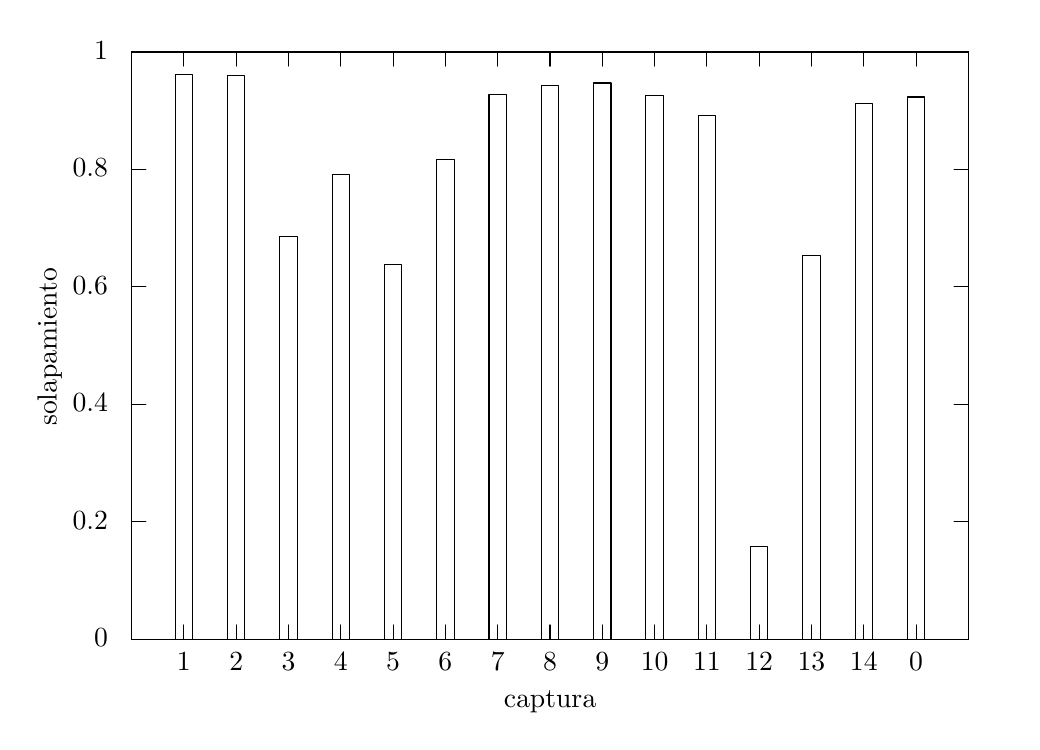
\begin{tikzpicture}[gnuplot]
%% generated with GNUPLOT 5.4p0 (Lua 5.4; terminal rev. Jun 2020, script rev. 114)
%% Tue 25 Aug 2020 01:55:34 AM -03
\gpmonochromelines
\path (0.000,0.000) rectangle (12.500,8.750);
\gpcolor{color=gp lt color border}
\gpsetlinetype{gp lt border}
\gpsetdashtype{gp dt solid}
\gpsetlinewidth{1.00}
\draw[gp path] (1.320,0.985)--(1.500,0.985);
\draw[gp path] (11.947,0.985)--(11.767,0.985);
\node[gp node right] at (1.136,0.985) {$0$};
\draw[gp path] (1.320,2.476)--(1.500,2.476);
\draw[gp path] (11.947,2.476)--(11.767,2.476);
\node[gp node right] at (1.136,2.476) {$0.2$};
\draw[gp path] (1.320,3.967)--(1.500,3.967);
\draw[gp path] (11.947,3.967)--(11.767,3.967);
\node[gp node right] at (1.136,3.967) {$0.4$};
\draw[gp path] (1.320,5.459)--(1.500,5.459);
\draw[gp path] (11.947,5.459)--(11.767,5.459);
\node[gp node right] at (1.136,5.459) {$0.6$};
\draw[gp path] (1.320,6.950)--(1.500,6.950);
\draw[gp path] (11.947,6.950)--(11.767,6.950);
\node[gp node right] at (1.136,6.950) {$0.8$};
\draw[gp path] (1.320,8.441)--(1.500,8.441);
\draw[gp path] (11.947,8.441)--(11.767,8.441);
\node[gp node right] at (1.136,8.441) {$1$};
\draw[gp path] (1.984,0.985)--(1.984,1.165);
\draw[gp path] (1.984,8.441)--(1.984,8.261);
\node[gp node center] at (1.984,0.677) {1};
\draw[gp path] (2.648,0.985)--(2.648,1.165);
\draw[gp path] (2.648,8.441)--(2.648,8.261);
\node[gp node center] at (2.648,0.677) {2};
\draw[gp path] (3.313,0.985)--(3.313,1.165);
\draw[gp path] (3.313,8.441)--(3.313,8.261);
\node[gp node center] at (3.313,0.677) {3};
\draw[gp path] (3.977,0.985)--(3.977,1.165);
\draw[gp path] (3.977,8.441)--(3.977,8.261);
\node[gp node center] at (3.977,0.677) {4};
\draw[gp path] (4.641,0.985)--(4.641,1.165);
\draw[gp path] (4.641,8.441)--(4.641,8.261);
\node[gp node center] at (4.641,0.677) {5};
\draw[gp path] (5.305,0.985)--(5.305,1.165);
\draw[gp path] (5.305,8.441)--(5.305,8.261);
\node[gp node center] at (5.305,0.677) {6};
\draw[gp path] (5.969,0.985)--(5.969,1.165);
\draw[gp path] (5.969,8.441)--(5.969,8.261);
\node[gp node center] at (5.969,0.677) {7};
\draw[gp path] (6.634,0.985)--(6.634,1.165);
\draw[gp path] (6.634,8.441)--(6.634,8.261);
\node[gp node center] at (6.634,0.677) {8};
\draw[gp path] (7.298,0.985)--(7.298,1.165);
\draw[gp path] (7.298,8.441)--(7.298,8.261);
\node[gp node center] at (7.298,0.677) {9};
\draw[gp path] (7.962,0.985)--(7.962,1.165);
\draw[gp path] (7.962,8.441)--(7.962,8.261);
\node[gp node center] at (7.962,0.677) {10};
\draw[gp path] (8.626,0.985)--(8.626,1.165);
\draw[gp path] (8.626,8.441)--(8.626,8.261);
\node[gp node center] at (8.626,0.677) {11};
\draw[gp path] (9.290,0.985)--(9.290,1.165);
\draw[gp path] (9.290,8.441)--(9.290,8.261);
\node[gp node center] at (9.290,0.677) {12};
\draw[gp path] (9.954,0.985)--(9.954,1.165);
\draw[gp path] (9.954,8.441)--(9.954,8.261);
\node[gp node center] at (9.954,0.677) {13};
\draw[gp path] (10.619,0.985)--(10.619,1.165);
\draw[gp path] (10.619,8.441)--(10.619,8.261);
\node[gp node center] at (10.619,0.677) {14};
\draw[gp path] (11.283,0.985)--(11.283,1.165);
\draw[gp path] (11.283,8.441)--(11.283,8.261);
\node[gp node center] at (11.283,0.677) {0};
\draw[gp path] (1.320,8.441)--(1.320,0.985)--(11.947,0.985)--(11.947,8.441)--cycle;
\node[gp node center,rotate=-270] at (0.292,4.713) {solapamiento};
\node[gp node center] at (6.633,0.215) {captura};
\draw[gp path] (1.873,0.985)--(1.873,8.158)--(2.095,8.158)--(2.095,0.985)--cycle;
\draw[gp path] (2.538,0.985)--(2.538,8.144)--(2.759,8.144)--(2.759,0.985)--cycle;
\draw[gp path] (3.202,0.985)--(3.202,6.102)--(3.423,6.102)--(3.423,0.985)--cycle;
\draw[gp path] (3.866,0.985)--(3.866,6.882)--(4.087,6.882)--(4.087,0.985)--cycle;
\draw[gp path] (4.530,0.985)--(4.530,5.745)--(4.752,5.745)--(4.752,0.985)--cycle;
\draw[gp path] (5.194,0.985)--(5.194,7.078)--(5.416,7.078)--(5.416,0.985)--cycle;
\draw[gp path] (5.859,0.985)--(5.859,7.902)--(6.080,7.902)--(6.080,0.985)--cycle;
\draw[gp path] (6.523,0.985)--(6.523,8.015)--(6.744,8.015)--(6.744,0.985)--cycle;
\draw[gp path] (7.187,0.985)--(7.187,8.047)--(7.408,8.047)--(7.408,0.985)--cycle;
\draw[gp path] (7.851,0.985)--(7.851,7.892)--(8.073,7.892)--(8.073,0.985)--cycle;
\draw[gp path] (8.515,0.985)--(8.515,7.634)--(8.737,7.634)--(8.737,0.985)--cycle;
\draw[gp path] (9.180,0.985)--(9.180,2.163)--(9.401,2.163)--(9.401,0.985)--cycle;
\draw[gp path] (9.844,0.985)--(9.844,5.858)--(10.065,5.858)--(10.065,0.985)--cycle;
\draw[gp path] (10.508,0.985)--(10.508,7.788)--(10.729,7.788)--(10.729,0.985)--cycle;
\draw[gp path] (11.172,0.985)--(11.172,7.869)--(11.394,7.869)--(11.394,0.985)--cycle;
\draw[gp path] (1.320,8.441)--(1.320,0.985)--(11.947,0.985)--(11.947,8.441)--cycle;
%% coordinates of the plot area
\gpdefrectangularnode{gp plot 1}{\pgfpoint{1.320cm}{0.985cm}}{\pgfpoint{11.947cm}{8.441cm}}
\end{tikzpicture}
%% gnuplot variables
}
				\resizebox{\linewidth}{!}{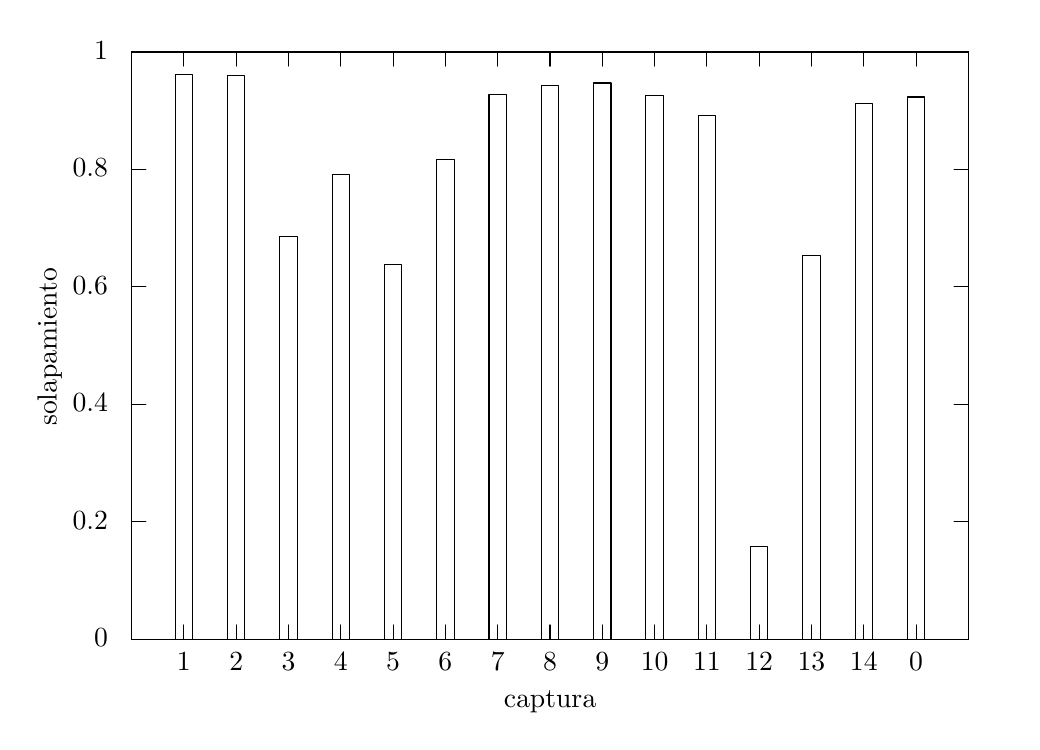
\begin{tikzpicture}[gnuplot]
%% generated with GNUPLOT 5.4p0 (Lua 5.4; terminal rev. Jun 2020, script rev. 114)
%% Tue 25 Aug 2020 01:55:34 AM -03
\gpmonochromelines
\path (0.000,0.000) rectangle (12.500,8.750);
\gpcolor{color=gp lt color border}
\gpsetlinetype{gp lt border}
\gpsetdashtype{gp dt solid}
\gpsetlinewidth{1.00}
\draw[gp path] (1.320,0.985)--(1.500,0.985);
\draw[gp path] (11.947,0.985)--(11.767,0.985);
\node[gp node right] at (1.136,0.985) {$0$};
\draw[gp path] (1.320,2.476)--(1.500,2.476);
\draw[gp path] (11.947,2.476)--(11.767,2.476);
\node[gp node right] at (1.136,2.476) {$0.2$};
\draw[gp path] (1.320,3.967)--(1.500,3.967);
\draw[gp path] (11.947,3.967)--(11.767,3.967);
\node[gp node right] at (1.136,3.967) {$0.4$};
\draw[gp path] (1.320,5.459)--(1.500,5.459);
\draw[gp path] (11.947,5.459)--(11.767,5.459);
\node[gp node right] at (1.136,5.459) {$0.6$};
\draw[gp path] (1.320,6.950)--(1.500,6.950);
\draw[gp path] (11.947,6.950)--(11.767,6.950);
\node[gp node right] at (1.136,6.950) {$0.8$};
\draw[gp path] (1.320,8.441)--(1.500,8.441);
\draw[gp path] (11.947,8.441)--(11.767,8.441);
\node[gp node right] at (1.136,8.441) {$1$};
\draw[gp path] (1.984,0.985)--(1.984,1.165);
\draw[gp path] (1.984,8.441)--(1.984,8.261);
\node[gp node center] at (1.984,0.677) {1};
\draw[gp path] (2.648,0.985)--(2.648,1.165);
\draw[gp path] (2.648,8.441)--(2.648,8.261);
\node[gp node center] at (2.648,0.677) {2};
\draw[gp path] (3.313,0.985)--(3.313,1.165);
\draw[gp path] (3.313,8.441)--(3.313,8.261);
\node[gp node center] at (3.313,0.677) {3};
\draw[gp path] (3.977,0.985)--(3.977,1.165);
\draw[gp path] (3.977,8.441)--(3.977,8.261);
\node[gp node center] at (3.977,0.677) {4};
\draw[gp path] (4.641,0.985)--(4.641,1.165);
\draw[gp path] (4.641,8.441)--(4.641,8.261);
\node[gp node center] at (4.641,0.677) {5};
\draw[gp path] (5.305,0.985)--(5.305,1.165);
\draw[gp path] (5.305,8.441)--(5.305,8.261);
\node[gp node center] at (5.305,0.677) {6};
\draw[gp path] (5.969,0.985)--(5.969,1.165);
\draw[gp path] (5.969,8.441)--(5.969,8.261);
\node[gp node center] at (5.969,0.677) {7};
\draw[gp path] (6.634,0.985)--(6.634,1.165);
\draw[gp path] (6.634,8.441)--(6.634,8.261);
\node[gp node center] at (6.634,0.677) {8};
\draw[gp path] (7.298,0.985)--(7.298,1.165);
\draw[gp path] (7.298,8.441)--(7.298,8.261);
\node[gp node center] at (7.298,0.677) {9};
\draw[gp path] (7.962,0.985)--(7.962,1.165);
\draw[gp path] (7.962,8.441)--(7.962,8.261);
\node[gp node center] at (7.962,0.677) {10};
\draw[gp path] (8.626,0.985)--(8.626,1.165);
\draw[gp path] (8.626,8.441)--(8.626,8.261);
\node[gp node center] at (8.626,0.677) {11};
\draw[gp path] (9.290,0.985)--(9.290,1.165);
\draw[gp path] (9.290,8.441)--(9.290,8.261);
\node[gp node center] at (9.290,0.677) {12};
\draw[gp path] (9.954,0.985)--(9.954,1.165);
\draw[gp path] (9.954,8.441)--(9.954,8.261);
\node[gp node center] at (9.954,0.677) {13};
\draw[gp path] (10.619,0.985)--(10.619,1.165);
\draw[gp path] (10.619,8.441)--(10.619,8.261);
\node[gp node center] at (10.619,0.677) {14};
\draw[gp path] (11.283,0.985)--(11.283,1.165);
\draw[gp path] (11.283,8.441)--(11.283,8.261);
\node[gp node center] at (11.283,0.677) {0};
\draw[gp path] (1.320,8.441)--(1.320,0.985)--(11.947,0.985)--(11.947,8.441)--cycle;
\node[gp node center,rotate=-270] at (0.292,4.713) {solapamiento};
\node[gp node center] at (6.633,0.215) {captura};
\draw[gp path] (1.873,0.985)--(1.873,8.158)--(2.095,8.158)--(2.095,0.985)--cycle;
\draw[gp path] (2.538,0.985)--(2.538,8.144)--(2.759,8.144)--(2.759,0.985)--cycle;
\draw[gp path] (3.202,0.985)--(3.202,6.102)--(3.423,6.102)--(3.423,0.985)--cycle;
\draw[gp path] (3.866,0.985)--(3.866,6.882)--(4.087,6.882)--(4.087,0.985)--cycle;
\draw[gp path] (4.530,0.985)--(4.530,5.745)--(4.752,5.745)--(4.752,0.985)--cycle;
\draw[gp path] (5.194,0.985)--(5.194,7.078)--(5.416,7.078)--(5.416,0.985)--cycle;
\draw[gp path] (5.859,0.985)--(5.859,7.902)--(6.080,7.902)--(6.080,0.985)--cycle;
\draw[gp path] (6.523,0.985)--(6.523,8.015)--(6.744,8.015)--(6.744,0.985)--cycle;
\draw[gp path] (7.187,0.985)--(7.187,8.047)--(7.408,8.047)--(7.408,0.985)--cycle;
\draw[gp path] (7.851,0.985)--(7.851,7.892)--(8.073,7.892)--(8.073,0.985)--cycle;
\draw[gp path] (8.515,0.985)--(8.515,7.634)--(8.737,7.634)--(8.737,0.985)--cycle;
\draw[gp path] (9.180,0.985)--(9.180,2.163)--(9.401,2.163)--(9.401,0.985)--cycle;
\draw[gp path] (9.844,0.985)--(9.844,5.858)--(10.065,5.858)--(10.065,0.985)--cycle;
\draw[gp path] (10.508,0.985)--(10.508,7.788)--(10.729,7.788)--(10.729,0.985)--cycle;
\draw[gp path] (11.172,0.985)--(11.172,7.869)--(11.394,7.869)--(11.394,0.985)--cycle;
\draw[gp path] (1.320,8.441)--(1.320,0.985)--(11.947,0.985)--(11.947,8.441)--cycle;
%% coordinates of the plot area
\gpdefrectangularnode{gp plot 1}{\pgfpoint{1.320cm}{0.985cm}}{\pgfpoint{11.947cm}{8.441cm}}
\end{tikzpicture}
%% gnuplot variables
}
			\caption{\label{fig:fitness}Métrica de alineación para el modelo \texttt{dragon stand}. El bajo
			porcentaje de solapamiento en la captura 12 se corresponde
			con un error de registración.}
		\end{figure}



		Como medida de error de la fusión se utilizó la distancia entre los puntos de la nube reconstruida
		respecto al punto más cercano en el \emph{ground truth} (cuadro~\ref{tab:fus_error}).
		La reconstrucción del modelo \texttt{armadillo} se encontraba a otra
		escala, por lo que no fue utilizada.
		Nuevamente se destaca el error de \texttt{dragon stand} producto de una mala alineación.

		\begin{table}
	\center
	\begin{tabular}{l*{3}{c}}
		\toprule                                                                  
		Modelo                  &    Error promedio  & Desvío \\ 
		\midrule                                    
		bunny                   &      1.28464       & 0.74131\\
		\midrule                                    
		dragon side             &      1.19651       & 0.69846\\
		dragon stand            &      2.83930       & 2.41398\\
		dragon up               &      1.14363       & 0.88966\\
		\midrule                                    
		drill (contra vrip)     &      1.48515       & 0.96336\\
		drill (contra zip)      &      1.74326       & 1.39883\\
		\midrule                                    
		happy back              &      1.65632       & 1.27056\\
		happy side              &      1.35371       & 1.01163\\
		happy stand             &      1.79513       & 1.25758\\
		\bottomrule                                                               
	\end{tabular}
	\caption{\label{tab:fus_error}Errores en la fusión.}
\end{table}



		%gráficos drill y front/back
		%En el caso de \texttt{drill}, 

		%solo front/back
		Se observa, además, una inflación/deflación de los objetos
		reconstruidos debida a la propagación del error de alineación.  Así, la
		primera captura coincide casi exactamente, pero el error se incrementa
		a medida que nos alejamos de ella (figura~\ref{fig:fus_happy}).

		\begin{figure}
			\Imagen{happy_diff}
			\caption{\label{fig:fus_happy}Diferencia contra el \emph{ground truth} del modelo \texttt{happy}.}
		\end{figure}


		%rellenado de huecos poisson
		Luego de aplicar el método de Poisson para rellenar los huecos, se
		obtuvieron las reconstrucciones que se observan en la
		figura~\ref{fig:poiss_all}.
		Los desperfectos observados en bunny (figura~\ref{fig:bun_ear}) se deben a una mala registración
		de la captura \texttt{bun180}, que se encontraba aproximadamente a
		$90^{\circ}$ respecto a sus vecinos.
		En cuanto a drill (figura~\ref{fig:drill_drops}), se tienen componentes
		inconexas debido a una mala fusión en una zona de alta curvatura.
		En todos los casos, la base de apoyo del objeto presenta una
		deformación hacia abajo (figura~\ref{fig:base}) con un hueco al final.
		Esto podría solucionarse mediante un preproceso rellenando la base con,
		por ejemplo, el método de \emph{advancing front}.

		\begin{figure}
			\Imagen{img/models_b}
			\caption{\label{fig:poiss_all}Resultado de las reconstrucciones luego del rellenado de huecos mediante el método de Poisson.
			Fila superior:
			De izquierda a derecha, y de arriba a abajo, los modelos son: armadillo, bunny, dragon, drill y happy.}
		\end{figure}

		\begin{figure}
			\centering
			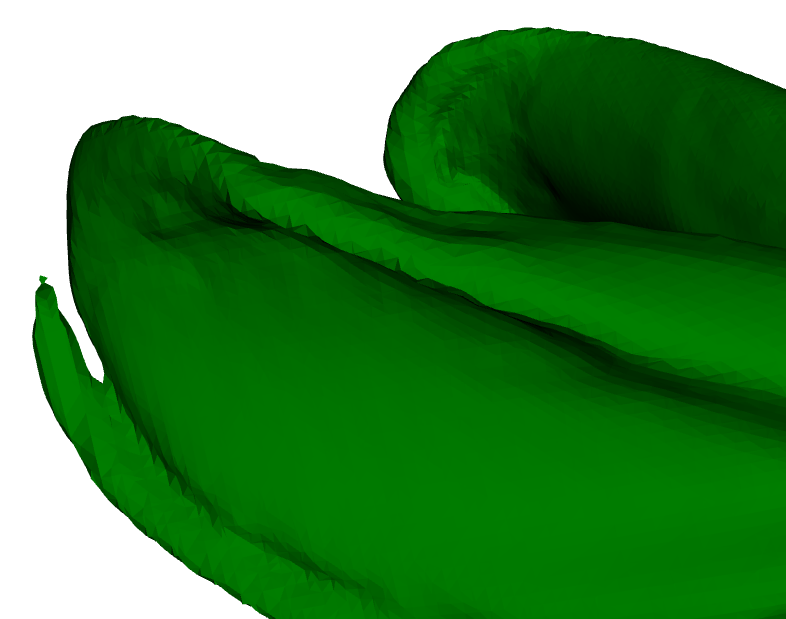
\includegraphics[max width=.5\linewidth, max height=.25\textheight, keepaspectratio]
				{img/bunny_ear}
			%\Imagen{img/bunny_ear}
			\caption{\label{fig:bun_ear}Acercamiento a la oreja derecha de bunny.}
		\end{figure}

		\begin{figure}
			%\Imagen{img/drill_drops}
			\centering
			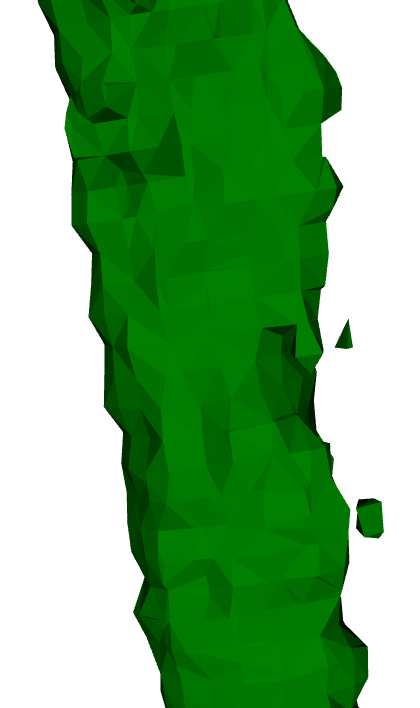
\includegraphics[max width=.5\linewidth, max height=.25\textheight, keepaspectratio]
				{img/drill_drops}
			\caption{\label{fig:drill_drops}Acercamiento a la mecha de drill. Se observan componentes inconexas con la malla principal.}
		\end{figure}

		\begin{figure}
			\centering
			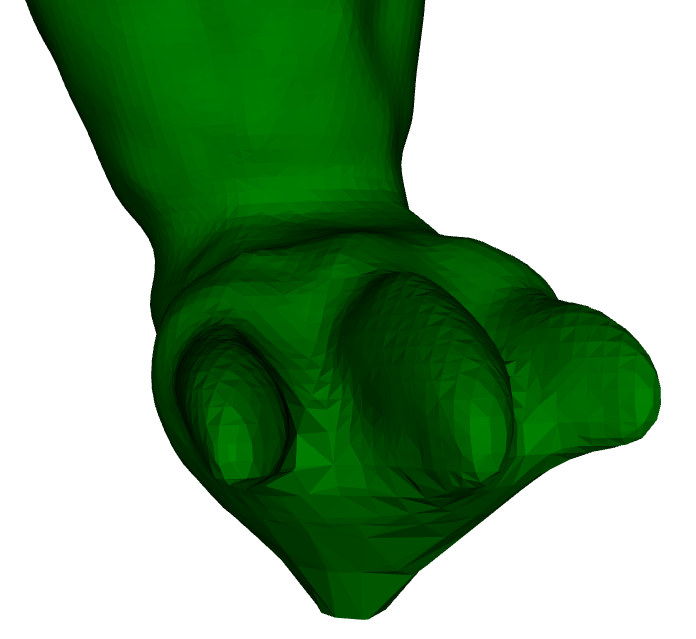
\includegraphics[max width=.5\linewidth, max height=.25\textheight, keepaspectratio]
				{img/arma_foot}
			%\Imagen{img/arma_foot}
			\caption{\label{fig:base}Acercamiento a la base de apoyo de armadillo. Se observa un estiramiento hacia abajo.}
		\end{figure}



	\section{Conclusiones}
		Como resultado de esta etapa se obtuvo una biblioteca de software que
		permite reconstruir un objeto tridimensional a partir de nubes
		de puntos de vistas parciales sujetas a ciertas restricciones.
		Debido al uso del método de Poisson en el rellenado, esta
		reconstrucción no presentará huecos, a excepción de la base de apoyo.

		Durante la registración, se obtuvieron resultados aceptables en casi todas las pruebas, 
		siendo uno de los fallos debido a un ángulo excesivo entre las tomas.
		Estos fallos pueden detectarse al utilizar la métrica de solapamiento y entonces proceder
		a ajustar los parámetros del algoritmo de alineación.

		A futuro se pretende desarrollar algoritmos que nos permitan relajar la
		restricción del eje de giro.
		De esta forma, se podrán combinar reconstrucciones del mismo objeto
		sobre la base de giro, con lo que se logrará recuperar la información
		perdida debido a oclusiones.




	\chapter{Pruebas y resultados}
\section{Pruebas parciales del módulo de registración}
%del capítulo de desarrollo
	Se realizaron pruebas preliminares de los métodos de alineación inicial
	de \emph{sample consensus} y búsqueda de \emph{clustering}
	sobre los objetos \texttt{happy} y \texttt{bunny}.
	Las capturas de \texttt{happy} se realizaron a intervalos de ángulos equiespaciados (cercanos a $24^{\circ}$) y
	presentan zonas suaves en la base, barriga y espalda.
	En cambio los ángulos en \texttt{bunny} son más variados y espaciados, yendo desde $35^{\circ}$ a $90^{\circ}$,
	y se observa una superficie más irregular por todo el cuerpo (figura~\ref{fig:stanford_models}).%\TODO{Sacar foto a los modelos}

	%SAC-IA
	En el caso de la alineación mediante \emph{sample consensus},
	se obtuvieron buenos resultados en la mayoría de las capturas de \texttt{happy}
	donde los ángulos eran cercanos a $25^{\circ}$ (figura~\ref{fig:sac_angles}).

	Pero al utilizar el modelo \texttt{bunny}, cuyos ángulos eran cercanos a $45^{\circ}$,
	se obtuvo una buena alineación en el caso de las capturas 315--000 y 000--045,
	sin embargo, para los otros casos las correspondencias fueron completamente erróneas (figura~\ref{fig:align_sac}).

	%Clustering
	Para el algoritmo de \emph{clustering}, en cambio,
	no se tuvieron problemas con el modelo \texttt{bunny},
	a pesar de presentar saltos cercanos a $90^{\circ}$ en las alineaciones
	contra la captura \texttt{bun180}. Si bien este salto supera las restricciones impuestas,
	en ningún caso se produjo una diferencia mayor a $5^{\circ}$ respecto al \emph{ground truth} (figura~\ref{fig:clust_bunny}).

	Para el modelo \texttt{happy} se obtuvieron resultados similares a pesar de que en este
	caso los ángulos eran más cercanos (aproximadamente $24^{\circ}$).  Las
	diferencias respecto al \emph{ground truth} no superaban los $5^{\circ}$,
	teniendo un error promedio de $2^{\circ}$ (figura~\ref{fig:clust_happy}).

	De esta forma, se logró acercar las capturas lo suficiente como
	para intentar alinearlas por ICP.


	\begin{figure}
		\TODO{unir con el de clustering}
		\Imagen{foo}
		\caption{\label{fig:sac_angles}\TODO{Diferencias entre la rotación estimada mediante \emph{sample consensus} y el \emph{ground truth} para el objeto \texttt{happy}}}
	\end{figure}


\begin{figure}
	%\Imagen{img/cluster_bunny}
	\resizebox{.9\linewidth}{!}{% Title: gl2ps_renderer figure
% Creator: GL2PS 1.4.0, (C) 1999-2017 C. Geuzaine
% For: Octave
% CreationDate: Wed Feb 26 13:03:30 2020
\begin{pgfpicture}
\color[rgb]{1.000000,1.000000,1.000000}
\pgfpathrectanglecorners{\pgfpoint{0pt}{0pt}}{\pgfpoint{576pt}{432pt}}
\pgfusepath{fill}
\begin{pgfscope}
\pgfpathrectangle{\pgfpoint{0pt}{0pt}}{\pgfpoint{576pt}{432pt}}
\pgfusepath{fill}
\pgfpathrectangle{\pgfpoint{0pt}{0pt}}{\pgfpoint{576pt}{432pt}}
\pgfusepath{clip}
\pgfpathmoveto{\pgfpoint{74.880020pt}{399.599976pt}}
\pgflineto{\pgfpoint{521.280029pt}{47.519989pt}}
\pgflineto{\pgfpoint{74.880020pt}{47.519989pt}}
\pgfpathclose
\pgfusepath{fill,stroke}
\pgfpathmoveto{\pgfpoint{74.880020pt}{399.599976pt}}
\pgflineto{\pgfpoint{521.280029pt}{399.599976pt}}
\pgflineto{\pgfpoint{521.280029pt}{47.519989pt}}
\pgfpathclose
\pgfusepath{fill,stroke}
\color[rgb]{0.150000,0.150000,0.150000}
\pgfsetlinewidth{0.500000pt}
\pgfpathmoveto{\pgfpoint{74.880020pt}{51.985016pt}}
\pgflineto{\pgfpoint{74.880020pt}{47.519989pt}}
\pgfusepath{stroke}
\pgfpathmoveto{\pgfpoint{74.880020pt}{395.134979pt}}
\pgflineto{\pgfpoint{74.880020pt}{399.599976pt}}
\pgfusepath{stroke}
\pgfpathmoveto{\pgfpoint{164.160019pt}{51.985016pt}}
\pgflineto{\pgfpoint{164.160019pt}{47.519989pt}}
\pgfusepath{stroke}
\pgfpathmoveto{\pgfpoint{164.160019pt}{395.134979pt}}
\pgflineto{\pgfpoint{164.160019pt}{399.599976pt}}
\pgfusepath{stroke}
\pgfpathmoveto{\pgfpoint{253.440018pt}{51.985016pt}}
\pgflineto{\pgfpoint{253.440018pt}{47.519989pt}}
\pgfusepath{stroke}
\pgfpathmoveto{\pgfpoint{253.440018pt}{395.134979pt}}
\pgflineto{\pgfpoint{253.440018pt}{399.599976pt}}
\pgfusepath{stroke}
\pgfpathmoveto{\pgfpoint{342.720032pt}{51.985016pt}}
\pgflineto{\pgfpoint{342.720032pt}{47.519989pt}}
\pgfusepath{stroke}
\pgfpathmoveto{\pgfpoint{342.720032pt}{395.134979pt}}
\pgflineto{\pgfpoint{342.720032pt}{399.599976pt}}
\pgfusepath{stroke}
\pgfpathmoveto{\pgfpoint{432.000000pt}{51.985016pt}}
\pgflineto{\pgfpoint{432.000000pt}{47.519989pt}}
\pgfusepath{stroke}
\pgfpathmoveto{\pgfpoint{432.000000pt}{395.134979pt}}
\pgflineto{\pgfpoint{432.000000pt}{399.599976pt}}
\pgfusepath{stroke}
\pgfpathmoveto{\pgfpoint{521.280029pt}{51.985016pt}}
\pgflineto{\pgfpoint{521.280029pt}{47.519989pt}}
\pgfusepath{stroke}
\pgfpathmoveto{\pgfpoint{521.280029pt}{395.134979pt}}
\pgflineto{\pgfpoint{521.280029pt}{399.599976pt}}
\pgfusepath{stroke}
{
\pgftransformshift{\pgfpoint{74.880005pt}{40.018295pt}}
\pgfnode{rectangle}{north}{\fontsize{10}{0}\selectfont\textcolor[rgb]{0.15,0.15,0.15}{{45}}}{}{\pgfusepath{discard}}}
{
\pgftransformshift{\pgfpoint{164.160004pt}{40.018295pt}}
\pgfnode{rectangle}{north}{\fontsize{10}{0}\selectfont\textcolor[rgb]{0.15,0.15,0.15}{{90}}}{}{\pgfusepath{discard}}}
{
\pgftransformshift{\pgfpoint{253.440002pt}{40.018295pt}}
\pgfnode{rectangle}{north}{\fontsize{10}{0}\selectfont\textcolor[rgb]{0.15,0.15,0.15}{{180}}}{}{\pgfusepath{discard}}}
{
\pgftransformshift{\pgfpoint{342.720001pt}{40.018295pt}}
\pgfnode{rectangle}{north}{\fontsize{10}{0}\selectfont\textcolor[rgb]{0.15,0.15,0.15}{{270}}}{}{\pgfusepath{discard}}}
{
\pgftransformshift{\pgfpoint{432.000000pt}{40.018295pt}}
\pgfnode{rectangle}{north}{\fontsize{10}{0}\selectfont\textcolor[rgb]{0.15,0.15,0.15}{{315}}}{}{\pgfusepath{discard}}}
{
\pgftransformshift{\pgfpoint{521.280029pt}{40.018295pt}}
\pgfnode{rectangle}{north}{\fontsize{10}{0}\selectfont\textcolor[rgb]{0.15,0.15,0.15}{{0}}}{}{\pgfusepath{discard}}}
\pgfpathmoveto{\pgfpoint{79.348038pt}{47.519989pt}}
\pgflineto{\pgfpoint{74.880020pt}{47.519989pt}}
\pgfusepath{stroke}
\pgfpathmoveto{\pgfpoint{516.812012pt}{47.519989pt}}
\pgflineto{\pgfpoint{521.280029pt}{47.519989pt}}
\pgfusepath{stroke}
\pgfpathmoveto{\pgfpoint{79.348038pt}{117.935997pt}}
\pgflineto{\pgfpoint{74.880020pt}{117.935997pt}}
\pgfusepath{stroke}
\pgfpathmoveto{\pgfpoint{516.812012pt}{117.935997pt}}
\pgflineto{\pgfpoint{521.280029pt}{117.935997pt}}
\pgfusepath{stroke}
\pgfpathmoveto{\pgfpoint{79.348038pt}{188.351990pt}}
\pgflineto{\pgfpoint{74.880020pt}{188.351990pt}}
\pgfusepath{stroke}
\pgfpathmoveto{\pgfpoint{516.812012pt}{188.351990pt}}
\pgflineto{\pgfpoint{521.280029pt}{188.351990pt}}
\pgfusepath{stroke}
\pgfpathmoveto{\pgfpoint{79.348038pt}{258.768005pt}}
\pgflineto{\pgfpoint{74.880020pt}{258.768005pt}}
\pgfusepath{stroke}
\pgfpathmoveto{\pgfpoint{516.812012pt}{258.768005pt}}
\pgflineto{\pgfpoint{521.280029pt}{258.768005pt}}
\pgfusepath{stroke}
\pgfpathmoveto{\pgfpoint{79.348038pt}{329.183990pt}}
\pgflineto{\pgfpoint{74.880020pt}{329.183990pt}}
\pgfusepath{stroke}
\pgfpathmoveto{\pgfpoint{516.812012pt}{329.183990pt}}
\pgflineto{\pgfpoint{521.280029pt}{329.183990pt}}
\pgfusepath{stroke}
\pgfpathmoveto{\pgfpoint{79.348038pt}{399.599976pt}}
\pgflineto{\pgfpoint{74.880020pt}{399.599976pt}}
\pgfusepath{stroke}
\pgfpathmoveto{\pgfpoint{516.812012pt}{399.599976pt}}
\pgflineto{\pgfpoint{521.280029pt}{399.599976pt}}
\pgfusepath{stroke}
{
\pgftransformshift{\pgfpoint{69.875519pt}{47.519989pt}}
\pgfnode{rectangle}{east}{\fontsize{10}{0}\selectfont\textcolor[rgb]{0.15,0.15,0.15}{{0}}}{}{\pgfusepath{discard}}}
{
\pgftransformshift{\pgfpoint{69.875519pt}{117.935989pt}}
\pgfnode{rectangle}{east}{\fontsize{10}{0}\selectfont\textcolor[rgb]{0.15,0.15,0.15}{{1}}}{}{\pgfusepath{discard}}}
{
\pgftransformshift{\pgfpoint{69.875519pt}{188.351990pt}}
\pgfnode{rectangle}{east}{\fontsize{10}{0}\selectfont\textcolor[rgb]{0.15,0.15,0.15}{{2}}}{}{\pgfusepath{discard}}}
{
\pgftransformshift{\pgfpoint{69.875519pt}{258.768005pt}}
\pgfnode{rectangle}{east}{\fontsize{10}{0}\selectfont\textcolor[rgb]{0.15,0.15,0.15}{{3}}}{}{\pgfusepath{discard}}}
{
\pgftransformshift{\pgfpoint{69.875519pt}{329.183990pt}}
\pgfnode{rectangle}{east}{\fontsize{10}{0}\selectfont\textcolor[rgb]{0.15,0.15,0.15}{{4}}}{}{\pgfusepath{discard}}}
{
\pgftransformshift{\pgfpoint{69.875519pt}{399.599976pt}}
\pgfnode{rectangle}{east}{\fontsize{10}{0}\selectfont\textcolor[rgb]{0.15,0.15,0.15}{{5}}}{}{\pgfusepath{discard}}}
\pgfsetrectcap
\pgfsetdash{{16pt}{0pt}}{0pt}
\pgfpathmoveto{\pgfpoint{521.280029pt}{47.519989pt}}
\pgflineto{\pgfpoint{74.880020pt}{47.519989pt}}
\pgfusepath{stroke}
\pgfpathmoveto{\pgfpoint{521.280029pt}{399.599976pt}}
\pgflineto{\pgfpoint{74.880020pt}{399.599976pt}}
\pgfusepath{stroke}
\pgfpathmoveto{\pgfpoint{74.880020pt}{399.599976pt}}
\pgflineto{\pgfpoint{74.880020pt}{47.519989pt}}
\pgfusepath{stroke}
\pgfpathmoveto{\pgfpoint{521.280029pt}{399.599976pt}}
\pgflineto{\pgfpoint{521.280029pt}{47.519989pt}}
\pgfusepath{stroke}
{
\pgftransformshift{\pgfpoint{298.079987pt}{27.018295pt}}
\pgfnode{rectangle}{north}{\fontsize{11}{0}\selectfont\textcolor[rgb]{0.15,0.15,0.15}{{captura}}}{}{\pgfusepath{discard}}}
{
\pgftransformshift{\pgfpoint{58.875519pt}{223.559998pt}}
\pgftransformrotate{90.000000}{\pgfnode{rectangle}{south}{\fontsize{11}{0}\selectfont\textcolor[rgb]{0.15,0.15,0.15}{{ángulo (grados)}}}{}{\pgfusepath{discard}}}}
\color[rgb]{0.000000,0.000000,0.000000}
\pgfsetbuttcap
\pgfsetroundjoin
\pgfsetdash{}{0pt}
\pgfpathmoveto{\pgfpoint{164.160019pt}{94.410004pt}}
\pgflineto{\pgfpoint{74.880020pt}{84.727814pt}}
\pgfusepath{stroke}
\pgfpathmoveto{\pgfpoint{253.440018pt}{338.880310pt}}
\pgflineto{\pgfpoint{164.160019pt}{94.410004pt}}
\pgfusepath{stroke}
\pgfpathmoveto{\pgfpoint{342.720032pt}{63.103058pt}}
\pgflineto{\pgfpoint{253.440018pt}{338.880310pt}}
\pgfusepath{stroke}
\pgfpathmoveto{\pgfpoint{432.000000pt}{193.823318pt}}
\pgflineto{\pgfpoint{342.720032pt}{63.103058pt}}
\pgfusepath{stroke}
\pgfpathmoveto{\pgfpoint{521.280029pt}{160.699646pt}}
\pgflineto{\pgfpoint{432.000000pt}{193.823318pt}}
\pgfusepath{stroke}
\pgfsetrectcap
\pgfsetmiterjoin
\pgfpathmoveto{\pgfpoint{77.880005pt}{84.727814pt}}
\pgflineto{\pgfpoint{71.879990pt}{84.727814pt}}
\pgfusepath{stroke}
\pgfpathmoveto{\pgfpoint{74.880005pt}{81.727814pt}}
\pgflineto{\pgfpoint{74.880005pt}{87.727814pt}}
\pgfusepath{stroke}
\pgfpathmoveto{\pgfpoint{77.001312pt}{82.606491pt}}
\pgflineto{\pgfpoint{72.758667pt}{86.849136pt}}
\pgfusepath{stroke}
\pgfpathmoveto{\pgfpoint{77.001312pt}{86.849136pt}}
\pgflineto{\pgfpoint{72.758667pt}{82.606491pt}}
\pgfusepath{stroke}
\pgfpathmoveto{\pgfpoint{167.160004pt}{94.410004pt}}
\pgflineto{\pgfpoint{161.160004pt}{94.410004pt}}
\pgfusepath{stroke}
\pgfpathmoveto{\pgfpoint{164.160004pt}{91.410004pt}}
\pgflineto{\pgfpoint{164.160004pt}{97.410011pt}}
\pgfusepath{stroke}
\pgfpathmoveto{\pgfpoint{166.281311pt}{92.288681pt}}
\pgflineto{\pgfpoint{162.038666pt}{96.531326pt}}
\pgfusepath{stroke}
\pgfpathmoveto{\pgfpoint{166.281311pt}{96.531326pt}}
\pgflineto{\pgfpoint{162.038666pt}{92.288681pt}}
\pgfusepath{stroke}
\pgfpathmoveto{\pgfpoint{256.440002pt}{338.880280pt}}
\pgflineto{\pgfpoint{250.440002pt}{338.880280pt}}
\pgfusepath{stroke}
\pgfpathmoveto{\pgfpoint{253.440002pt}{335.880280pt}}
\pgflineto{\pgfpoint{253.440002pt}{341.880280pt}}
\pgfusepath{stroke}
\pgfpathmoveto{\pgfpoint{255.561310pt}{336.758972pt}}
\pgflineto{\pgfpoint{251.318680pt}{341.001617pt}}
\pgfusepath{stroke}
\pgfpathmoveto{\pgfpoint{255.561310pt}{341.001617pt}}
\pgflineto{\pgfpoint{251.318680pt}{336.758972pt}}
\pgfusepath{stroke}
\pgfpathmoveto{\pgfpoint{345.720032pt}{63.103058pt}}
\pgflineto{\pgfpoint{339.720032pt}{63.103058pt}}
\pgfusepath{stroke}
\pgfpathmoveto{\pgfpoint{342.720032pt}{60.103058pt}}
\pgflineto{\pgfpoint{342.720032pt}{66.103073pt}}
\pgfusepath{stroke}
\pgfpathmoveto{\pgfpoint{344.841339pt}{60.981750pt}}
\pgflineto{\pgfpoint{340.598694pt}{65.224396pt}}
\pgfusepath{stroke}
\pgfpathmoveto{\pgfpoint{344.841339pt}{65.224396pt}}
\pgflineto{\pgfpoint{340.598694pt}{60.981750pt}}
\pgfusepath{stroke}
\pgfpathmoveto{\pgfpoint{435.000000pt}{193.823318pt}}
\pgflineto{\pgfpoint{429.000000pt}{193.823318pt}}
\pgfusepath{stroke}
\pgfpathmoveto{\pgfpoint{432.000000pt}{190.823318pt}}
\pgflineto{\pgfpoint{432.000000pt}{196.823318pt}}
\pgfusepath{stroke}
\pgfpathmoveto{\pgfpoint{434.121338pt}{191.701996pt}}
\pgflineto{\pgfpoint{429.878662pt}{195.944641pt}}
\pgfusepath{stroke}
\pgfpathmoveto{\pgfpoint{434.121338pt}{195.944641pt}}
\pgflineto{\pgfpoint{429.878662pt}{191.701996pt}}
\pgfusepath{stroke}
\pgfpathmoveto{\pgfpoint{524.280029pt}{160.699646pt}}
\pgflineto{\pgfpoint{518.280029pt}{160.699646pt}}
\pgfusepath{stroke}
\pgfpathmoveto{\pgfpoint{521.280029pt}{157.699646pt}}
\pgflineto{\pgfpoint{521.280029pt}{163.699646pt}}
\pgfusepath{stroke}
\pgfpathmoveto{\pgfpoint{523.401367pt}{158.578308pt}}
\pgflineto{\pgfpoint{519.158691pt}{162.820953pt}}
\pgfusepath{stroke}
\pgfpathmoveto{\pgfpoint{523.401367pt}{162.820953pt}}
\pgflineto{\pgfpoint{519.158691pt}{158.578308pt}}
\pgfusepath{stroke}
\end{pgfscope}
\end{pgfpicture}
}
	\caption{\label{fig:clust_bunny}Diferencias absolutas entre la rotación estimada y el \emph{ground truth} para el objeto \texttt{bunny}.}
\end{figure}

\begin{figure}
	%\Imagen{img/cluster_happy}
	\resizebox{.9\linewidth}{!}{% Title: gl2ps_renderer figure
% Creator: GL2PS 1.4.0, (C) 1999-2017 C. Geuzaine
% For: Octave
% CreationDate: Wed Feb 26 13:15:21 2020
\begin{pgfpicture}
\color[rgb]{1.000000,1.000000,1.000000}
\pgfpathrectanglecorners{\pgfpoint{0pt}{0pt}}{\pgfpoint{576pt}{432pt}}
\pgfusepath{fill}
\begin{pgfscope}
\pgfpathrectangle{\pgfpoint{0pt}{0pt}}{\pgfpoint{576pt}{432pt}}
\pgfusepath{fill}
\pgfpathrectangle{\pgfpoint{0pt}{0pt}}{\pgfpoint{576pt}{432pt}}
\pgfusepath{clip}
\pgfpathmoveto{\pgfpoint{74.880005pt}{399.599976pt}}
\pgflineto{\pgfpoint{521.279968pt}{47.519989pt}}
\pgflineto{\pgfpoint{74.880005pt}{47.519989pt}}
\pgfpathclose
\pgfusepath{fill,stroke}
\pgfpathmoveto{\pgfpoint{74.880005pt}{399.599976pt}}
\pgflineto{\pgfpoint{521.279968pt}{399.599976pt}}
\pgflineto{\pgfpoint{521.279968pt}{47.519989pt}}
\pgfpathclose
\pgfusepath{fill,stroke}
\color[rgb]{0.150000,0.150000,0.150000}
\pgfsetlinewidth{0.500000pt}
\pgfpathmoveto{\pgfpoint{106.765701pt}{51.985016pt}}
\pgflineto{\pgfpoint{106.765701pt}{47.519989pt}}
\pgfusepath{stroke}
\pgfpathmoveto{\pgfpoint{106.765701pt}{395.135010pt}}
\pgflineto{\pgfpoint{106.765701pt}{399.599976pt}}
\pgfusepath{stroke}
\pgfpathmoveto{\pgfpoint{170.537140pt}{51.985016pt}}
\pgflineto{\pgfpoint{170.537140pt}{47.519989pt}}
\pgfusepath{stroke}
\pgfpathmoveto{\pgfpoint{170.537140pt}{395.135010pt}}
\pgflineto{\pgfpoint{170.537140pt}{399.599976pt}}
\pgfusepath{stroke}
\pgfpathmoveto{\pgfpoint{234.308563pt}{51.985016pt}}
\pgflineto{\pgfpoint{234.308563pt}{47.519989pt}}
\pgfusepath{stroke}
\pgfpathmoveto{\pgfpoint{234.308563pt}{395.135010pt}}
\pgflineto{\pgfpoint{234.308563pt}{399.599976pt}}
\pgfusepath{stroke}
\pgfpathmoveto{\pgfpoint{298.079987pt}{51.985016pt}}
\pgflineto{\pgfpoint{298.079987pt}{47.519989pt}}
\pgfusepath{stroke}
\pgfpathmoveto{\pgfpoint{298.079987pt}{395.135010pt}}
\pgflineto{\pgfpoint{298.079987pt}{399.599976pt}}
\pgfusepath{stroke}
\pgfpathmoveto{\pgfpoint{361.851440pt}{51.985016pt}}
\pgflineto{\pgfpoint{361.851440pt}{47.519989pt}}
\pgfusepath{stroke}
\pgfpathmoveto{\pgfpoint{361.851440pt}{395.135010pt}}
\pgflineto{\pgfpoint{361.851440pt}{399.599976pt}}
\pgfusepath{stroke}
\pgfpathmoveto{\pgfpoint{425.622864pt}{51.985016pt}}
\pgflineto{\pgfpoint{425.622864pt}{47.519989pt}}
\pgfusepath{stroke}
\pgfpathmoveto{\pgfpoint{425.622864pt}{395.135010pt}}
\pgflineto{\pgfpoint{425.622864pt}{399.599976pt}}
\pgfusepath{stroke}
\pgfpathmoveto{\pgfpoint{489.394257pt}{51.985016pt}}
\pgflineto{\pgfpoint{489.394257pt}{47.519989pt}}
\pgfusepath{stroke}
\pgfpathmoveto{\pgfpoint{489.394257pt}{395.135010pt}}
\pgflineto{\pgfpoint{489.394257pt}{399.599976pt}}
\pgfusepath{stroke}
{
\pgftransformshift{\pgfpoint{106.765701pt}{40.018295pt}}
\pgfnode{rectangle}{north}{\fontsize{10}{0}\selectfont\textcolor[rgb]{0.15,0.15,0.15}{{2}}}{}{\pgfusepath{discard}}}
{
\pgftransformshift{\pgfpoint{170.537140pt}{40.018295pt}}
\pgfnode{rectangle}{north}{\fontsize{10}{0}\selectfont\textcolor[rgb]{0.15,0.15,0.15}{{4}}}{}{\pgfusepath{discard}}}
{
\pgftransformshift{\pgfpoint{234.308563pt}{40.018295pt}}
\pgfnode{rectangle}{north}{\fontsize{10}{0}\selectfont\textcolor[rgb]{0.15,0.15,0.15}{{6}}}{}{\pgfusepath{discard}}}
{
\pgftransformshift{\pgfpoint{298.079987pt}{40.018295pt}}
\pgfnode{rectangle}{north}{\fontsize{10}{0}\selectfont\textcolor[rgb]{0.15,0.15,0.15}{{8}}}{}{\pgfusepath{discard}}}
{
\pgftransformshift{\pgfpoint{361.851410pt}{40.018295pt}}
\pgfnode{rectangle}{north}{\fontsize{10}{0}\selectfont\textcolor[rgb]{0.15,0.15,0.15}{{10}}}{}{\pgfusepath{discard}}}
{
\pgftransformshift{\pgfpoint{425.622864pt}{40.018295pt}}
\pgfnode{rectangle}{north}{\fontsize{10}{0}\selectfont\textcolor[rgb]{0.15,0.15,0.15}{{12}}}{}{\pgfusepath{discard}}}
{
\pgftransformshift{\pgfpoint{489.394257pt}{40.018295pt}}
\pgfnode{rectangle}{north}{\fontsize{10}{0}\selectfont\textcolor[rgb]{0.15,0.15,0.15}{{14}}}{}{\pgfusepath{discard}}}
\pgfpathmoveto{\pgfpoint{79.347992pt}{119.599602pt}}
\pgflineto{\pgfpoint{74.880005pt}{119.599602pt}}
\pgfusepath{stroke}
\pgfpathmoveto{\pgfpoint{516.812012pt}{119.599602pt}}
\pgflineto{\pgfpoint{521.279968pt}{119.599602pt}}
\pgfusepath{stroke}
\pgfpathmoveto{\pgfpoint{79.347992pt}{192.628571pt}}
\pgflineto{\pgfpoint{74.880005pt}{192.628571pt}}
\pgfusepath{stroke}
\pgfpathmoveto{\pgfpoint{516.812012pt}{192.628571pt}}
\pgflineto{\pgfpoint{521.279968pt}{192.628571pt}}
\pgfusepath{stroke}
\pgfpathmoveto{\pgfpoint{79.347992pt}{265.657562pt}}
\pgflineto{\pgfpoint{74.880005pt}{265.657562pt}}
\pgfusepath{stroke}
\pgfpathmoveto{\pgfpoint{516.812012pt}{265.657562pt}}
\pgflineto{\pgfpoint{521.279968pt}{265.657562pt}}
\pgfusepath{stroke}
\pgfpathmoveto{\pgfpoint{79.347992pt}{338.686523pt}}
\pgflineto{\pgfpoint{74.880005pt}{338.686523pt}}
\pgfusepath{stroke}
\pgfpathmoveto{\pgfpoint{516.812012pt}{338.686523pt}}
\pgflineto{\pgfpoint{521.279968pt}{338.686523pt}}
\pgfusepath{stroke}
{
\pgftransformshift{\pgfpoint{69.875504pt}{119.599602pt}}
\pgfnode{rectangle}{east}{\fontsize{10}{0}\selectfont\textcolor[rgb]{0.15,0.15,0.15}{{1}}}{}{\pgfusepath{discard}}}
{
\pgftransformshift{\pgfpoint{69.875504pt}{192.628571pt}}
\pgfnode{rectangle}{east}{\fontsize{10}{0}\selectfont\textcolor[rgb]{0.15,0.15,0.15}{{2}}}{}{\pgfusepath{discard}}}
{
\pgftransformshift{\pgfpoint{69.875504pt}{265.657562pt}}
\pgfnode{rectangle}{east}{\fontsize{10}{0}\selectfont\textcolor[rgb]{0.15,0.15,0.15}{{3}}}{}{\pgfusepath{discard}}}
{
\pgftransformshift{\pgfpoint{69.875504pt}{338.686523pt}}
\pgfnode{rectangle}{east}{\fontsize{10}{0}\selectfont\textcolor[rgb]{0.15,0.15,0.15}{{4}}}{}{\pgfusepath{discard}}}
\pgfsetrectcap
\pgfsetdash{{16pt}{0pt}}{0pt}
\pgfpathmoveto{\pgfpoint{521.279968pt}{47.519989pt}}
\pgflineto{\pgfpoint{74.880005pt}{47.519989pt}}
\pgfusepath{stroke}
\pgfpathmoveto{\pgfpoint{521.279968pt}{399.599976pt}}
\pgflineto{\pgfpoint{74.880005pt}{399.599976pt}}
\pgfusepath{stroke}
\pgfpathmoveto{\pgfpoint{74.880005pt}{399.599976pt}}
\pgflineto{\pgfpoint{74.880005pt}{47.519989pt}}
\pgfusepath{stroke}
\pgfpathmoveto{\pgfpoint{521.279968pt}{399.599976pt}}
\pgflineto{\pgfpoint{521.279968pt}{47.519989pt}}
\pgfusepath{stroke}
{
\pgftransformshift{\pgfpoint{298.079987pt}{27.018295pt}}
\pgfnode{rectangle}{north}{\fontsize{11}{0}\selectfont\textcolor[rgb]{0.15,0.15,0.15}{{captura}}}{}{\pgfusepath{discard}}}
{
\pgftransformshift{\pgfpoint{58.875488pt}{223.559998pt}}
\pgftransformrotate{90.000000}{\pgfnode{rectangle}{south}{\fontsize{11}{0}\selectfont\textcolor[rgb]{0.15,0.15,0.15}{{ángulo (grados)}}}{}{\pgfusepath{discard}}}}
\color[rgb]{0.000000,0.000000,0.000000}
\pgfsetbuttcap
\pgfsetroundjoin
\pgfsetdash{}{0pt}
\pgfpathmoveto{\pgfpoint{106.765701pt}{104.614059pt}}
\pgflineto{\pgfpoint{74.880005pt}{78.732574pt}}
\pgfusepath{stroke}
\pgfpathmoveto{\pgfpoint{138.651413pt}{124.864990pt}}
\pgflineto{\pgfpoint{106.765701pt}{104.614059pt}}
\pgfusepath{stroke}
\pgfpathmoveto{\pgfpoint{170.537140pt}{347.625275pt}}
\pgflineto{\pgfpoint{138.651413pt}{124.864990pt}}
\pgfusepath{stroke}
\pgfpathmoveto{\pgfpoint{202.422852pt}{47.519989pt}}
\pgflineto{\pgfpoint{170.537140pt}{347.625275pt}}
\pgfusepath{stroke}
\pgfpathmoveto{\pgfpoint{234.308563pt}{248.838989pt}}
\pgflineto{\pgfpoint{202.422852pt}{47.519989pt}}
\pgfusepath{stroke}
\pgfpathmoveto{\pgfpoint{266.194275pt}{156.296661pt}}
\pgflineto{\pgfpoint{234.308563pt}{248.838989pt}}
\pgfusepath{stroke}
\pgfpathmoveto{\pgfpoint{298.079987pt}{52.624725pt}}
\pgflineto{\pgfpoint{266.194275pt}{156.296661pt}}
\pgfusepath{stroke}
\pgfpathmoveto{\pgfpoint{329.965698pt}{67.464203pt}}
\pgflineto{\pgfpoint{298.079987pt}{52.624725pt}}
\pgfusepath{stroke}
\pgfpathmoveto{\pgfpoint{361.851440pt}{204.094131pt}}
\pgflineto{\pgfpoint{329.965698pt}{67.464203pt}}
\pgfusepath{stroke}
\pgfpathmoveto{\pgfpoint{393.737122pt}{260.771912pt}}
\pgflineto{\pgfpoint{361.851440pt}{204.094131pt}}
\pgfusepath{stroke}
\pgfpathmoveto{\pgfpoint{425.622864pt}{399.599976pt}}
\pgflineto{\pgfpoint{393.737122pt}{260.771912pt}}
\pgfusepath{stroke}
\pgfpathmoveto{\pgfpoint{457.508575pt}{187.253632pt}}
\pgflineto{\pgfpoint{425.622864pt}{399.599976pt}}
\pgfusepath{stroke}
\pgfpathmoveto{\pgfpoint{489.394257pt}{313.433136pt}}
\pgflineto{\pgfpoint{457.508575pt}{187.253632pt}}
\pgfusepath{stroke}
\pgfpathmoveto{\pgfpoint{521.279968pt}{398.219757pt}}
\pgflineto{\pgfpoint{489.394257pt}{313.433136pt}}
\pgfusepath{stroke}
\pgfsetrectcap
\pgfsetmiterjoin
\pgfpathmoveto{\pgfpoint{77.880005pt}{78.732574pt}}
\pgflineto{\pgfpoint{71.879990pt}{78.732574pt}}
\pgfusepath{stroke}
\pgfpathmoveto{\pgfpoint{74.880005pt}{75.732574pt}}
\pgflineto{\pgfpoint{74.880005pt}{81.732574pt}}
\pgfusepath{stroke}
\pgfpathmoveto{\pgfpoint{77.001312pt}{76.611252pt}}
\pgflineto{\pgfpoint{72.758667pt}{80.853897pt}}
\pgfusepath{stroke}
\pgfpathmoveto{\pgfpoint{77.001312pt}{80.853897pt}}
\pgflineto{\pgfpoint{72.758667pt}{76.611252pt}}
\pgfusepath{stroke}
\pgfpathmoveto{\pgfpoint{109.765732pt}{104.614029pt}}
\pgflineto{\pgfpoint{103.765717pt}{104.614029pt}}
\pgfusepath{stroke}
\pgfpathmoveto{\pgfpoint{106.765717pt}{101.614029pt}}
\pgflineto{\pgfpoint{106.765717pt}{107.614029pt}}
\pgfusepath{stroke}
\pgfpathmoveto{\pgfpoint{108.887039pt}{102.492706pt}}
\pgflineto{\pgfpoint{104.644394pt}{106.735352pt}}
\pgfusepath{stroke}
\pgfpathmoveto{\pgfpoint{108.887039pt}{106.735352pt}}
\pgflineto{\pgfpoint{104.644394pt}{102.492706pt}}
\pgfusepath{stroke}
\pgfpathmoveto{\pgfpoint{141.651428pt}{124.864983pt}}
\pgflineto{\pgfpoint{135.651428pt}{124.864983pt}}
\pgfusepath{stroke}
\pgfpathmoveto{\pgfpoint{138.651428pt}{121.864983pt}}
\pgflineto{\pgfpoint{138.651428pt}{127.864983pt}}
\pgfusepath{stroke}
\pgfpathmoveto{\pgfpoint{140.772751pt}{122.743660pt}}
\pgflineto{\pgfpoint{136.530106pt}{126.986305pt}}
\pgfusepath{stroke}
\pgfpathmoveto{\pgfpoint{140.772751pt}{126.986305pt}}
\pgflineto{\pgfpoint{136.530106pt}{122.743660pt}}
\pgfusepath{stroke}
\pgfpathmoveto{\pgfpoint{173.537140pt}{347.625305pt}}
\pgflineto{\pgfpoint{167.537155pt}{347.625305pt}}
\pgfusepath{stroke}
\pgfpathmoveto{\pgfpoint{170.537140pt}{344.625275pt}}
\pgflineto{\pgfpoint{170.537140pt}{350.625305pt}}
\pgfusepath{stroke}
\pgfpathmoveto{\pgfpoint{172.658478pt}{345.503967pt}}
\pgflineto{\pgfpoint{168.415833pt}{349.746613pt}}
\pgfusepath{stroke}
\pgfpathmoveto{\pgfpoint{172.658478pt}{349.746613pt}}
\pgflineto{\pgfpoint{168.415833pt}{345.503967pt}}
\pgfusepath{stroke}
\pgfpathmoveto{\pgfpoint{205.422852pt}{47.519974pt}}
\pgflineto{\pgfpoint{199.422852pt}{47.519974pt}}
\pgfusepath{stroke}
\pgfpathmoveto{\pgfpoint{202.422852pt}{44.519974pt}}
\pgflineto{\pgfpoint{202.422852pt}{50.519989pt}}
\pgfusepath{stroke}
\pgfpathmoveto{\pgfpoint{204.544174pt}{45.398651pt}}
\pgflineto{\pgfpoint{200.301529pt}{49.641296pt}}
\pgfusepath{stroke}
\pgfpathmoveto{\pgfpoint{204.544174pt}{49.641296pt}}
\pgflineto{\pgfpoint{200.301529pt}{45.398651pt}}
\pgfusepath{stroke}
\pgfpathmoveto{\pgfpoint{237.308578pt}{248.838959pt}}
\pgflineto{\pgfpoint{231.308578pt}{248.838959pt}}
\pgfusepath{stroke}
\pgfpathmoveto{\pgfpoint{234.308578pt}{245.838959pt}}
\pgflineto{\pgfpoint{234.308578pt}{251.838974pt}}
\pgfusepath{stroke}
\pgfpathmoveto{\pgfpoint{236.429901pt}{246.717651pt}}
\pgflineto{\pgfpoint{232.187256pt}{250.960281pt}}
\pgfusepath{stroke}
\pgfpathmoveto{\pgfpoint{236.429901pt}{250.960281pt}}
\pgflineto{\pgfpoint{232.187256pt}{246.717651pt}}
\pgfusepath{stroke}
\pgfpathmoveto{\pgfpoint{269.194275pt}{156.296661pt}}
\pgflineto{\pgfpoint{263.194275pt}{156.296661pt}}
\pgfusepath{stroke}
\pgfpathmoveto{\pgfpoint{266.194275pt}{153.296661pt}}
\pgflineto{\pgfpoint{266.194275pt}{159.296661pt}}
\pgfusepath{stroke}
\pgfpathmoveto{\pgfpoint{268.315613pt}{154.175323pt}}
\pgflineto{\pgfpoint{264.072968pt}{158.417969pt}}
\pgfusepath{stroke}
\pgfpathmoveto{\pgfpoint{268.315613pt}{158.417969pt}}
\pgflineto{\pgfpoint{264.072968pt}{154.175323pt}}
\pgfusepath{stroke}
\pgfpathmoveto{\pgfpoint{301.079987pt}{52.624741pt}}
\pgflineto{\pgfpoint{295.079987pt}{52.624741pt}}
\pgfusepath{stroke}
\pgfpathmoveto{\pgfpoint{298.079987pt}{49.624741pt}}
\pgflineto{\pgfpoint{298.079987pt}{55.624741pt}}
\pgfusepath{stroke}
\pgfpathmoveto{\pgfpoint{300.201324pt}{50.503418pt}}
\pgflineto{\pgfpoint{295.958679pt}{54.746063pt}}
\pgfusepath{stroke}
\pgfpathmoveto{\pgfpoint{300.201324pt}{54.746063pt}}
\pgflineto{\pgfpoint{295.958679pt}{50.503418pt}}
\pgfusepath{stroke}
\pgfpathmoveto{\pgfpoint{332.965759pt}{67.464203pt}}
\pgflineto{\pgfpoint{326.965759pt}{67.464203pt}}
\pgfusepath{stroke}
\pgfpathmoveto{\pgfpoint{329.965759pt}{64.464203pt}}
\pgflineto{\pgfpoint{329.965759pt}{70.464203pt}}
\pgfusepath{stroke}
\pgfpathmoveto{\pgfpoint{332.087067pt}{65.342880pt}}
\pgflineto{\pgfpoint{327.844421pt}{69.585526pt}}
\pgfusepath{stroke}
\pgfpathmoveto{\pgfpoint{332.087067pt}{69.585526pt}}
\pgflineto{\pgfpoint{327.844421pt}{65.342880pt}}
\pgfusepath{stroke}
\pgfpathmoveto{\pgfpoint{364.851440pt}{204.094131pt}}
\pgflineto{\pgfpoint{358.851440pt}{204.094131pt}}
\pgfusepath{stroke}
\pgfpathmoveto{\pgfpoint{361.851440pt}{201.094131pt}}
\pgflineto{\pgfpoint{361.851440pt}{207.094131pt}}
\pgfusepath{stroke}
\pgfpathmoveto{\pgfpoint{363.972778pt}{201.972809pt}}
\pgflineto{\pgfpoint{359.730103pt}{206.215454pt}}
\pgfusepath{stroke}
\pgfpathmoveto{\pgfpoint{363.972778pt}{206.215454pt}}
\pgflineto{\pgfpoint{359.730103pt}{201.972809pt}}
\pgfusepath{stroke}
\pgfpathmoveto{\pgfpoint{396.737152pt}{260.771912pt}}
\pgflineto{\pgfpoint{390.737152pt}{260.771912pt}}
\pgfusepath{stroke}
\pgfpathmoveto{\pgfpoint{393.737152pt}{257.771912pt}}
\pgflineto{\pgfpoint{393.737152pt}{263.771912pt}}
\pgfusepath{stroke}
\pgfpathmoveto{\pgfpoint{395.858490pt}{258.650574pt}}
\pgflineto{\pgfpoint{391.615845pt}{262.893219pt}}
\pgfusepath{stroke}
\pgfpathmoveto{\pgfpoint{395.858490pt}{262.893219pt}}
\pgflineto{\pgfpoint{391.615845pt}{258.650574pt}}
\pgfusepath{stroke}
\pgfpathmoveto{\pgfpoint{428.622864pt}{399.600006pt}}
\pgflineto{\pgfpoint{422.622864pt}{399.600006pt}}
\pgfusepath{stroke}
\pgfpathmoveto{\pgfpoint{425.622864pt}{396.600006pt}}
\pgflineto{\pgfpoint{425.622864pt}{402.600006pt}}
\pgfusepath{stroke}
\pgfpathmoveto{\pgfpoint{427.744202pt}{397.478699pt}}
\pgflineto{\pgfpoint{423.501556pt}{401.721313pt}}
\pgfusepath{stroke}
\pgfpathmoveto{\pgfpoint{427.744202pt}{401.721313pt}}
\pgflineto{\pgfpoint{423.501556pt}{397.478699pt}}
\pgfusepath{stroke}
\pgfpathmoveto{\pgfpoint{460.508575pt}{187.253632pt}}
\pgflineto{\pgfpoint{454.508545pt}{187.253632pt}}
\pgfusepath{stroke}
\pgfpathmoveto{\pgfpoint{457.508575pt}{184.253632pt}}
\pgflineto{\pgfpoint{457.508575pt}{190.253632pt}}
\pgfusepath{stroke}
\pgfpathmoveto{\pgfpoint{459.629883pt}{185.132324pt}}
\pgflineto{\pgfpoint{455.387268pt}{189.374954pt}}
\pgfusepath{stroke}
\pgfpathmoveto{\pgfpoint{459.629883pt}{189.374954pt}}
\pgflineto{\pgfpoint{455.387268pt}{185.132324pt}}
\pgfusepath{stroke}
\pgfpathmoveto{\pgfpoint{492.394287pt}{313.433105pt}}
\pgflineto{\pgfpoint{486.394287pt}{313.433105pt}}
\pgfusepath{stroke}
\pgfpathmoveto{\pgfpoint{489.394287pt}{310.433105pt}}
\pgflineto{\pgfpoint{489.394287pt}{316.433105pt}}
\pgfusepath{stroke}
\pgfpathmoveto{\pgfpoint{491.515625pt}{311.311798pt}}
\pgflineto{\pgfpoint{487.272980pt}{315.554443pt}}
\pgfusepath{stroke}
\pgfpathmoveto{\pgfpoint{491.515625pt}{315.554443pt}}
\pgflineto{\pgfpoint{487.272980pt}{311.311798pt}}
\pgfusepath{stroke}
\pgfpathmoveto{\pgfpoint{524.280029pt}{398.219757pt}}
\pgflineto{\pgfpoint{518.280029pt}{398.219757pt}}
\pgfusepath{stroke}
\pgfpathmoveto{\pgfpoint{521.280029pt}{395.219757pt}}
\pgflineto{\pgfpoint{521.280029pt}{401.219757pt}}
\pgfusepath{stroke}
\pgfpathmoveto{\pgfpoint{523.401367pt}{396.098450pt}}
\pgflineto{\pgfpoint{519.158691pt}{400.341064pt}}
\pgfusepath{stroke}
\pgfpathmoveto{\pgfpoint{523.401367pt}{400.341064pt}}
\pgflineto{\pgfpoint{519.158691pt}{396.098450pt}}
\pgfusepath{stroke}
\end{pgfscope}
\end{pgfpicture}
}
	\caption{\label{fig:clust_happy}Diferencias absolutas entre la rotación estimada y el \emph{ground truth} para el objeto \texttt{happy}.}
\end{figure}

\begin{figure}
	\centering
	\begin{subfigure}{.8\linewidth}
		\Imagen{img/bun_sac_270_315}
		\caption{\label{fig:align_sac}Ejemplo de fallo del algoritmo de \emph{sample consensus} producto de malas correspondencias.}
	\end{subfigure}
	\begin{subfigure}{.8\linewidth}
		\Imagen{img/bun_clust_270_315}
		\caption{\label{fig:clust_bun_good}Alineación exitosa mediante el uso de marcos de referencia.}
	\end{subfigure}
	\caption{Alineación entre las capturas \texttt{bun270} (verde) y \texttt{bun315} (rojo).}
\end{figure}

\section{Pruebas parciales del módulo de rellenado de huecos}
\subsection{Advancing front}
		%mover a resultados
		Con este método se pueden rellenar agujeros pequeños, obteniéndose una malla regular (figura~\ref{fig:fill_good}).
		Sin embargo, debido a la localidad con la que se generan los nuevos
		puntos, el frente puede diverger o pretender unirse a puntos que no
		forman parte del contorno del hueco, resultando una malla mal formada,
		con aristas que corresponden a más de dos caras (figura~\ref{fig:fill_bad}).
		Para evitar la divergencia es necesario definir una superficie de
		soporte considerando todo el contorno del hueco, de forma de asegurar
		que los nuevos puntos no excedan los límites del hueco.

	\begin{figure}
		\Imagen{img/fill_good}
		\caption{\label{fig:fill_good}Relleno de un hueco pequeño mediante \emph{advancing front}.}
	\end{figure}

	\begin{figure}
		\Imagen{img/fill_bad}
		\caption{\label{fig:fill_bad}Fallo en el algoritmo de \emph{advancing front}. Se intentó completar un triángulo con un punto que no pertenecía al borde.}
		\TODO{cambiar gráfico}
	\end{figure}


	\section{Introducción}
	En esta etapa se integraron los módulos de registración, fusión y rellenado de huecos,
	para resolver todas las funcionalidades propuestas por el proyecto.
	Con el fin de analizar el rendimiento del sistema,
	se utilizaron los modelos provistos por la base de datos Stanford.

	\section{Integración}
		El principal problema para la integración fue lograr la comunicación
		entre los módulos.  Según la metodología incremental elegida para la
		etapa de desarrollo, el diseño del módulo de fusión se inició luego de
		que el módulo de registración estuviera implementado, y de la misma
		manera, el diseño del módulo de rellenado de huecos se inició luego de
		obtener la implementación del de fusión. 
		Por esta razón, podría resultar prohibitivamente costoso modificar el diseño de un módulo anterior.

		Este problema se hizo evidente al establecer el formato de nube utilizado en cada módulo.
		Para la registración fue conveniente, en un primer momento,
		que la información de posición y normal de cada punto de la nube se encontrase por separado,
		por lo que al implementar las diversas alternativas se siguió manteniendo este formato.
		Sin embargo, los algoritmos de fusión y rellenado de huecos requerían
		que esta información estuviera junta.

		Debido a que ya se contaba con los resultados de la registración, es
		decir, con las transformaciones de las vistas, se idearon funciones de
		conversión entre esos dos formatos de nubes.
		Sin embargo, se planea una posterior modificación del módulo de registración de
		forma que las conversiones sean transparentes para el usuario de la
		biblioteca.

		Con respecto al módulo de rellenado de huecos, debido a los algoritmos
		utilizados, ocurre una pérdida de información de los resultados de la
		fusión:
		\begin{itemize}
			\item El método de \emph{advancing front} descarta todos aquellos
				puntos que no pertenezcan a la mayor componente conexa de la
				triangulación. Esto se realiza para evitar la presencia de islas y así
				simplificar la implementación del método.
				Una versión futura podría evitar esta pérdida de información.

			\item En el caso del método de \emph{Poisson}, las conectividades entre los
				puntos es completamente ignorada, lo cual ocasiona uniones erróneas en algunos casos.
		\end{itemize}


	\section{Funcionalidades}
		A continuación se describirán las funcionalidades que provee el sistema
		para dar respuesta a los requerimientos identificados en etapas
		previas.

		\begin{itemize}
			\item  \NombreItem{Preproceso}
				Se realizó una reducción de ruido al ajustar los puntos
				mediante el algoritmo de mínimos cuadrados móviles.

			\item  \NombreItem{Outliers}
				El ruido y los puntos extremos se consideran en varias etapas de la reconstrucción.
				Durante el preproceso, una triangulación Delaunay identifica y elimina puntos extremos.
				Durante la fusión, los puntos sin confirmación o de poca confianza
				se consideran provenientes del ruido.
				Antes de realizar el rellenado de huecos, pueden eliminarse
				componentes que contengan pocos puntos.

			\item  \NombreItem{Registración}
				Se proveen dos métodos para la alineación inicial en el módulo de registración:
				uno basado en \emph{sample consensus} de puntos salientes, y el otro basado en
				búsqueda de clústers según el marco de referencia ISS.
				Además, se cuenta con un refinamiento posterior mediante ICP.

			\item  \NombreItem{Área solapada}
				El área solapada  entre dos nubes
				se definió como aquellos puntos que estén a menos de un umbral de distancia
				al punto más cercano en la otra nube.
				Para realizar la búsqueda eficientemente se utilizó un k-d tree.

			\item  \NombreItem{Métricas}
				Cómo métricas de calidad de la registración se utilizaron
				la distancia entre las nubes considerando sólo el área solapada,
				y la razón entre la cantidad de puntos de la nube de entrada con esta área solapada.

			\item  \NombreItem{Corrección de bucle}
				El error de alineación del bucle se define como la
				transformación total calculada para ajustar la primer captura a la última
				una vez completada una vuelta. Debido a que la primer captura definió el
				marco de referencia, en una registración perfecta esta
				transformación sería la identidad.
				Calculando su inversa se obtiene una corrección que será distribuida
				a las otras registraciones.

			\item  \NombreItem{Combinación de nubes}
				El módulo de fusión provee esta funcionalidad, utilizando una
				representación de surfel con visibilidad, confianza y vecindad.

			\item  \NombreItem{Triangulación tridimensional}
				La triangulación se realiza mediante el método de \emph{Greedy
				Projection Triangulation} provisto por PCL.
				Se estableció un umbral en el tamaño de los triángulos considerando la resolución de la nube,
				así como también límites para sus ángulos.

			\item  \NombreItem{Identificación de huecos}
				Las conectividades de la malla se almacenan en un grafo de medias aristas.
				Los huecos se identifican como aquellas aristas que inciden en sólo una cara.
				Se hizo uso de \texttt{PCL::getBoundBoundary} transformando su resultado para
				obtener los puntos del contorno del hueco y ordenarlos según su tamaño
				(cantidad de puntos).

			\item  \NombreItem{Rellenado de huecos}
				Se da respuesta a esta funcionalidad mediante los algoritmos de \emph{advancing front} y reconstrucción de Poisson.
		\end{itemize}


		Como dependencias externas se tienen:
		\begin{itemize}
			\item PCL\footnote{\url{http://www.pointclouds.org/}},
				para el procesamiento de las nubes de puntos;
			\item delaunator-cpp\footnote{\url{https://github.com/delfrrr/delaunator-cpp}}, para la triangulación Delaunay;
			\item DKM\footnote{\url{https://github.com/genbattle/dkm}}, para el algoritmo de k-means.
		\end{itemize}
		Debido a que el sistema hace uso únicamente de bibliotecas multiplataforma,
		se garantiza su funcionamiento tanto en Linux como Windows.

	\section{Pruebas}
		Para realizar las pruebas se utilizaron los modelos
			armadillo,
			bunny,
			dragon,
			drill y
			happy del repositorio de Stanford\footnote{\url{http://graphics.stanford.edu/data/3Dscanrep/}}.
		Para cada modelo se tienen capturas realizadas sobre una base giratoria
		a diversos ángulos, en algunos casos en varias posiciones, y
		algunas capturas de ciertos detalles.
		Para cada captura se tiene, ademas, la transformación de alineación que
		la lleva a un sistema de referencia global.
		El repositorio cuenta también con los objetos reconstruidos utilizando
		todas las capturas disponibles.
		Se estableció entonces el \emph{ground truth} como el conjunto de estas
		transformaciones de alineación y el objeto reconstruido.

		Para la registración se utilizó el método basado en la búsqueda de clúster,
		seguido de un refinamiento mediante ICP y una corrección de bucle.
		En la fusión se utilizó una distancia de proximidad de $1.5$ veces la resolución de las nubes,
		y un mínimo de confianza de $0.2$.
		El rellenado de huecos se realizó mediante el método de Poisson.


		Durante el proceso de reconstrucción, se observa que la etapa de reconstrucción
		es responsable de la mayor parte del costo computacional, sobre todo al aumentar
		la cantidad de puntos en las capturas (cuadro~\ref{tab:reconstr_time}).
		En el cuadro~\ref{tab:reg_time} se muestran
		los tiempos de ejecución promedio, discriminados en la alineación
		inicial y el refinamiento posterior.
		Graficando estos tiempos se puede apreciar el orden $\bigO(n^2)$ de la alineación inicial,
		producto de buscar entre todos los pares de puntos para establecer las correspondencias.
		%Si bien los tiempos no son considerables, pueden reducirse al mejorar
		%la selección inicial de puntos y realizar la búsqueda de las
		%correspondencias de forma más eficiente.
		\begin{table}
	\centering
	\begin{tabular}{l*{6}{r}}
		\toprule
		Modelo                 & Puntos   & Capturas  &  Registración & Fusión   & Rellenado & Total\\
		\midrule
		armadillo back         &  25e3    &   11      &   84.4308        & 10.759  &  8.562  & 103.752\\
		armadillo head         &  25e3    &   12      &   114.4926       & 12.501  &  9.892  & 136.886\\
		armadillo head offset  &  25e3    &   11      &   100.7846       & 11.987  &  9.718  & 122.490\\
		armadillo stand        &  25e3    &   12      &   102.3553       & 12.145  &  9.498  & 123.998\\
		armadillo stand flip   &  25e3    &   11      &   101.7061       & 12.958  &  9.280  & 123.944\\
		\midrule
		bunny                  &  35e3    &   6       &    92.2872       & 11.246  &  11.862 & 115.395\\
		\midrule
		dragon side            &  20e3    &   15      &   90.5427        & 14.021  &  8.086  & 112.650\\
		dragon stand           &  30e3    &   15      &   180.8010       & 23.485  &  12.680 & 216.966\\
		dragon up              &  30e3    &   15      &   164.1075       & 18.469  &  9.669  & 192.245\\
		\midrule
		drill                  &   4e3    &   12      &   4.3172         & 1.988   &  4.176  & 10.481 \\
		\midrule
		happy back             &  45e3    &   15      &   343.2705       & 29.618  &  7.528  & 380.417\\
		happy side             &  45e3    &   15      &   452.5830       & 32.588  &  8.361  & 493.532\\
		happy stand            &  75e3    &   15      &   907.2930       & 44.570  &  10.929 & 962.792\\
		\bottomrule
	\end{tabular}
	\caption[Tiempo de reconstrucción]{\label{tab:reconstr_time}Tiempo de reconstrucción por cada modelo (en segundos).}
\end{table}


		\TODO{análisis de escabilidad, ver orden $n^2$}

		\begin{table}
	\centering
	\begin{tabular}{l*{4}{c}}
		\toprule
		Modelo                 &  Puntos  &   Inicial (s)  &   ICP  (s)  &  Total  (s)\\
		\midrule
		armadillo\\
		{\Em}back         &  25e3    &       7.05694    &   0.618592  &    7.67553\\
		{\Em}head         &  25e3    &       8.94947    &   0.591576  &    9.54105\\
		{\Em}head offset  &  25e3    &       8.62241    &   0.539835  &    9.16224\\
		{\Em}stand        &  25e3    &       7.98686    &   0.542746  &    8.52961\\
		{\Em}stand flip   &  25e3    &       8.69949    &   0.546518  &    9.24601\\
		\midrule
		bunny                  &  35e3    &       14.0323    &   1.348890  &    15.3812\\
		\midrule
		dragon\\
		{\Em}side            &  20e3    &       5.52965    &   0.506529  &    6.03618\\
		{\Em}stand           &  30e3    &       11.3732    &   0.680195  &    12.0534\\
		{\Em}up              &  30e3    &       10.3322    &   0.608282  &    10.9405\\
		\midrule
		drill                  &   4e3    &       0.26898    &   0.090796  &    0.35977\\
		\midrule
		happy\\
		{\Em}back             &  45e3    &       21.2702    &   1.614520  &    22.8847\\
		{\Em}side             &  45e3    &       29.1103    &   1.061880  &    30.1722\\
		{\Em}stand            &  75e3    &       59.3281    &   1.158030  &    60.4862\\
		\bottomrule
	\end{tabular}
	\caption[Tiempos de ejecución promedio para la registración]{\label{tab:reg_time}Tiempos de ejecución promedio para la
	registración de a pares en los distintos modelos.}
\end{table}


		\TODO{imagen del proceso}
		Para comparar las alineaciones contra el \emph{ground truth}, se
		observó el efecto de las mismas sobre un punto orientado (simulando la
		cámara). El punto \emph{eye} se ubicó inicialmente en las coordenadas
		$\{0, -0.1, 0.7\}$ (valores obtenidos de la base de datos), y se
		orientó el vector \emph{target} hacia $-z$ y el \emph{up} hacia $y$.
		El error de posicionamiento es la razón entre la distancia al punto
		de inicio y la distancia al punto obtenido por el \emph{ground truth}.
		En el caso de \emph{target} y \emph{up}, se midió el ángulo contra los
		vectores obtenidos por el \emph{ground truth}.

		Los errores de la registración se observan en el
		cuadro~\ref{tab:reg_error}.  Los errores no superan $1^{\circ}$ en
		orientación ni $1\%$ en posicionamiento.  Se da una excepción en el
		caso de \texttt{dragon stand}, debido a una mala alineación en la
		captura 12 (figura~\ref{fig:fitness}).

		\begin{table}
	\centering
	\begin{tabular}{l*{3}{c}}
		\toprule                                                                  
		Modelo                   &    Eye          &    Target (grados)        &    Up (grados)\\
		\midrule
		armadillo back          &     0.0062159   &   0.221725     &    ---\\        
		armadillo head          &     0.0036356  &    0.102321     &    0.211231\\   
		armadillo head offset   &     0.0029806  &    0.086309     &    0.229574\\   
		armadillo stand         &     0.0022145  &    0.049612     &    0.105862\\   
		armadillo stand flip    &     0.0045019  &    0.125330     &    0.146033\\   
		\midrule
		bunny                   &     0.0104809   &   0.598354     &    0.817185\\   
		\midrule
		dragon side             &     0.0070872  &    0.178650     &    0.212932\\   
		dragon stand            &     0.0536199   &   1.379760     &    0.207754\\   
		dragon up               &     0.0058265  &    0.139297     &    ---\\        
		\midrule
		drill                   &     0.0082317  &    0.238639     &    0.100126\\   
		\midrule
		happy back              &     0.0088540  &    0.189885     &    0.207247\\   
		happy side              &     0.0072675   &   0.175860     &    ---\\        
		happy stand             &     0.0050124  &    0.101383     &    0.097800\\  
		\bottomrule                                                               
	\end{tabular}
	\caption[Errores de registración]{\label{tab:reg_error}Errores de registración.
	\TODO{¿por qué hay vacíos?}}
\end{table}


		\begin{figure}
			\center
				%\scalebox{.75}{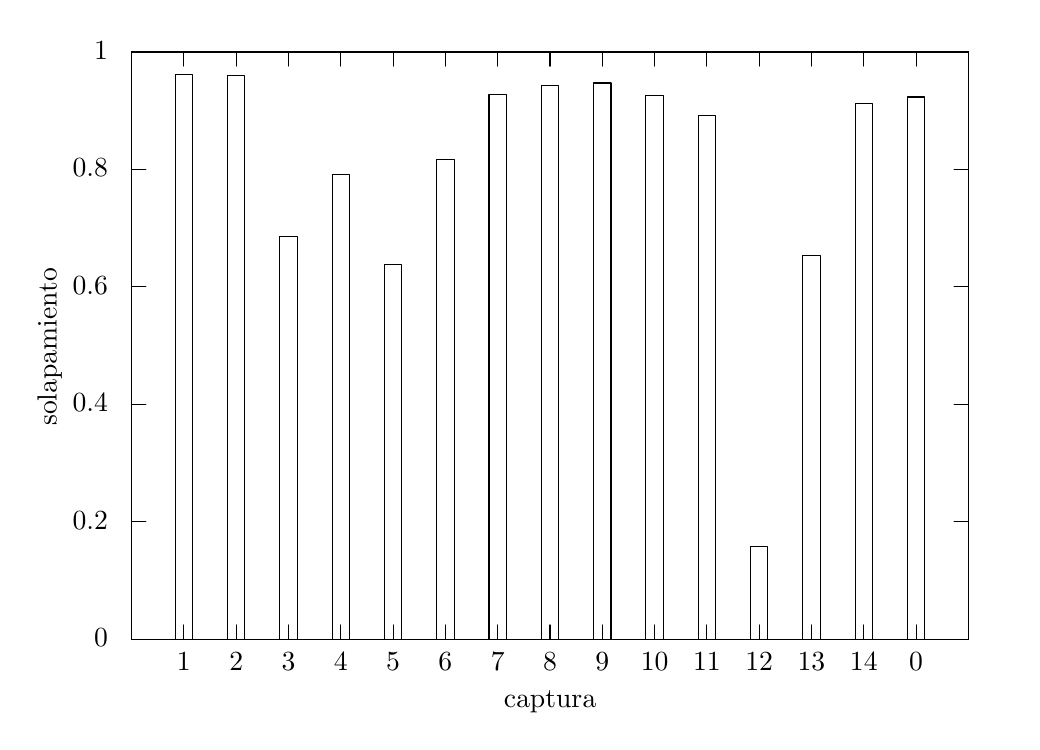
\begin{tikzpicture}[gnuplot]
%% generated with GNUPLOT 5.4p0 (Lua 5.4; terminal rev. Jun 2020, script rev. 114)
%% Tue 25 Aug 2020 01:55:34 AM -03
\gpmonochromelines
\path (0.000,0.000) rectangle (12.500,8.750);
\gpcolor{color=gp lt color border}
\gpsetlinetype{gp lt border}
\gpsetdashtype{gp dt solid}
\gpsetlinewidth{1.00}
\draw[gp path] (1.320,0.985)--(1.500,0.985);
\draw[gp path] (11.947,0.985)--(11.767,0.985);
\node[gp node right] at (1.136,0.985) {$0$};
\draw[gp path] (1.320,2.476)--(1.500,2.476);
\draw[gp path] (11.947,2.476)--(11.767,2.476);
\node[gp node right] at (1.136,2.476) {$0.2$};
\draw[gp path] (1.320,3.967)--(1.500,3.967);
\draw[gp path] (11.947,3.967)--(11.767,3.967);
\node[gp node right] at (1.136,3.967) {$0.4$};
\draw[gp path] (1.320,5.459)--(1.500,5.459);
\draw[gp path] (11.947,5.459)--(11.767,5.459);
\node[gp node right] at (1.136,5.459) {$0.6$};
\draw[gp path] (1.320,6.950)--(1.500,6.950);
\draw[gp path] (11.947,6.950)--(11.767,6.950);
\node[gp node right] at (1.136,6.950) {$0.8$};
\draw[gp path] (1.320,8.441)--(1.500,8.441);
\draw[gp path] (11.947,8.441)--(11.767,8.441);
\node[gp node right] at (1.136,8.441) {$1$};
\draw[gp path] (1.984,0.985)--(1.984,1.165);
\draw[gp path] (1.984,8.441)--(1.984,8.261);
\node[gp node center] at (1.984,0.677) {1};
\draw[gp path] (2.648,0.985)--(2.648,1.165);
\draw[gp path] (2.648,8.441)--(2.648,8.261);
\node[gp node center] at (2.648,0.677) {2};
\draw[gp path] (3.313,0.985)--(3.313,1.165);
\draw[gp path] (3.313,8.441)--(3.313,8.261);
\node[gp node center] at (3.313,0.677) {3};
\draw[gp path] (3.977,0.985)--(3.977,1.165);
\draw[gp path] (3.977,8.441)--(3.977,8.261);
\node[gp node center] at (3.977,0.677) {4};
\draw[gp path] (4.641,0.985)--(4.641,1.165);
\draw[gp path] (4.641,8.441)--(4.641,8.261);
\node[gp node center] at (4.641,0.677) {5};
\draw[gp path] (5.305,0.985)--(5.305,1.165);
\draw[gp path] (5.305,8.441)--(5.305,8.261);
\node[gp node center] at (5.305,0.677) {6};
\draw[gp path] (5.969,0.985)--(5.969,1.165);
\draw[gp path] (5.969,8.441)--(5.969,8.261);
\node[gp node center] at (5.969,0.677) {7};
\draw[gp path] (6.634,0.985)--(6.634,1.165);
\draw[gp path] (6.634,8.441)--(6.634,8.261);
\node[gp node center] at (6.634,0.677) {8};
\draw[gp path] (7.298,0.985)--(7.298,1.165);
\draw[gp path] (7.298,8.441)--(7.298,8.261);
\node[gp node center] at (7.298,0.677) {9};
\draw[gp path] (7.962,0.985)--(7.962,1.165);
\draw[gp path] (7.962,8.441)--(7.962,8.261);
\node[gp node center] at (7.962,0.677) {10};
\draw[gp path] (8.626,0.985)--(8.626,1.165);
\draw[gp path] (8.626,8.441)--(8.626,8.261);
\node[gp node center] at (8.626,0.677) {11};
\draw[gp path] (9.290,0.985)--(9.290,1.165);
\draw[gp path] (9.290,8.441)--(9.290,8.261);
\node[gp node center] at (9.290,0.677) {12};
\draw[gp path] (9.954,0.985)--(9.954,1.165);
\draw[gp path] (9.954,8.441)--(9.954,8.261);
\node[gp node center] at (9.954,0.677) {13};
\draw[gp path] (10.619,0.985)--(10.619,1.165);
\draw[gp path] (10.619,8.441)--(10.619,8.261);
\node[gp node center] at (10.619,0.677) {14};
\draw[gp path] (11.283,0.985)--(11.283,1.165);
\draw[gp path] (11.283,8.441)--(11.283,8.261);
\node[gp node center] at (11.283,0.677) {0};
\draw[gp path] (1.320,8.441)--(1.320,0.985)--(11.947,0.985)--(11.947,8.441)--cycle;
\node[gp node center,rotate=-270] at (0.292,4.713) {solapamiento};
\node[gp node center] at (6.633,0.215) {captura};
\draw[gp path] (1.873,0.985)--(1.873,8.158)--(2.095,8.158)--(2.095,0.985)--cycle;
\draw[gp path] (2.538,0.985)--(2.538,8.144)--(2.759,8.144)--(2.759,0.985)--cycle;
\draw[gp path] (3.202,0.985)--(3.202,6.102)--(3.423,6.102)--(3.423,0.985)--cycle;
\draw[gp path] (3.866,0.985)--(3.866,6.882)--(4.087,6.882)--(4.087,0.985)--cycle;
\draw[gp path] (4.530,0.985)--(4.530,5.745)--(4.752,5.745)--(4.752,0.985)--cycle;
\draw[gp path] (5.194,0.985)--(5.194,7.078)--(5.416,7.078)--(5.416,0.985)--cycle;
\draw[gp path] (5.859,0.985)--(5.859,7.902)--(6.080,7.902)--(6.080,0.985)--cycle;
\draw[gp path] (6.523,0.985)--(6.523,8.015)--(6.744,8.015)--(6.744,0.985)--cycle;
\draw[gp path] (7.187,0.985)--(7.187,8.047)--(7.408,8.047)--(7.408,0.985)--cycle;
\draw[gp path] (7.851,0.985)--(7.851,7.892)--(8.073,7.892)--(8.073,0.985)--cycle;
\draw[gp path] (8.515,0.985)--(8.515,7.634)--(8.737,7.634)--(8.737,0.985)--cycle;
\draw[gp path] (9.180,0.985)--(9.180,2.163)--(9.401,2.163)--(9.401,0.985)--cycle;
\draw[gp path] (9.844,0.985)--(9.844,5.858)--(10.065,5.858)--(10.065,0.985)--cycle;
\draw[gp path] (10.508,0.985)--(10.508,7.788)--(10.729,7.788)--(10.729,0.985)--cycle;
\draw[gp path] (11.172,0.985)--(11.172,7.869)--(11.394,7.869)--(11.394,0.985)--cycle;
\draw[gp path] (1.320,8.441)--(1.320,0.985)--(11.947,0.985)--(11.947,8.441)--cycle;
%% coordinates of the plot area
\gpdefrectangularnode{gp plot 1}{\pgfpoint{1.320cm}{0.985cm}}{\pgfpoint{11.947cm}{8.441cm}}
\end{tikzpicture}
%% gnuplot variables
}
				\resizebox{\linewidth}{!}{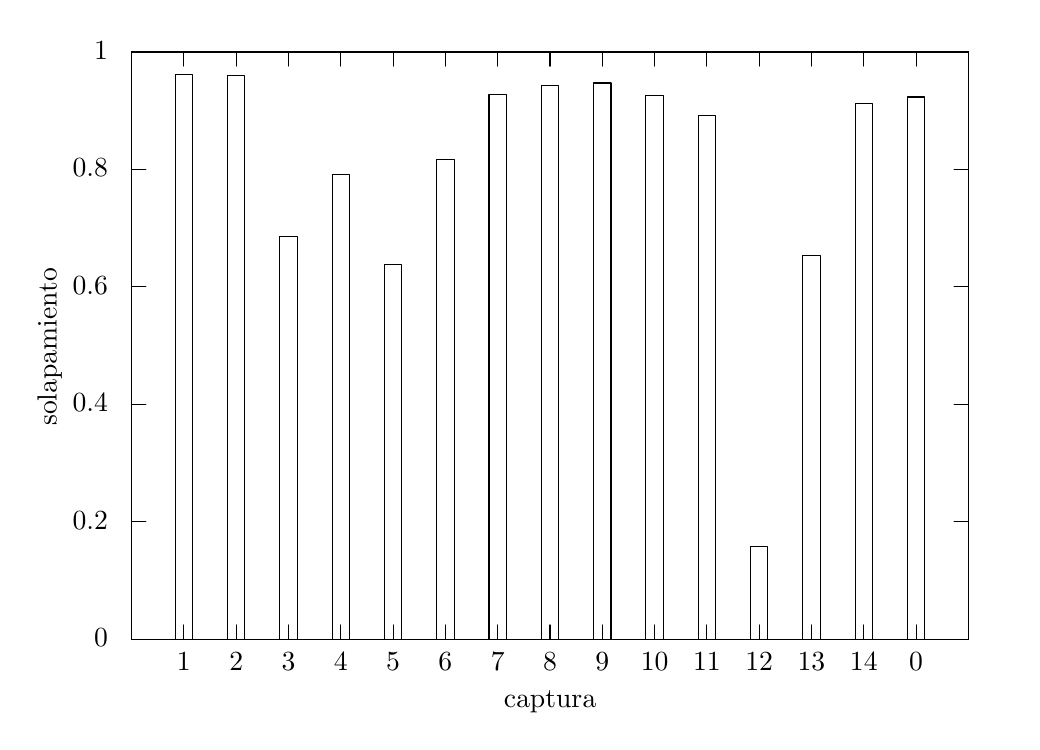
\begin{tikzpicture}[gnuplot]
%% generated with GNUPLOT 5.4p0 (Lua 5.4; terminal rev. Jun 2020, script rev. 114)
%% Tue 25 Aug 2020 01:55:34 AM -03
\gpmonochromelines
\path (0.000,0.000) rectangle (12.500,8.750);
\gpcolor{color=gp lt color border}
\gpsetlinetype{gp lt border}
\gpsetdashtype{gp dt solid}
\gpsetlinewidth{1.00}
\draw[gp path] (1.320,0.985)--(1.500,0.985);
\draw[gp path] (11.947,0.985)--(11.767,0.985);
\node[gp node right] at (1.136,0.985) {$0$};
\draw[gp path] (1.320,2.476)--(1.500,2.476);
\draw[gp path] (11.947,2.476)--(11.767,2.476);
\node[gp node right] at (1.136,2.476) {$0.2$};
\draw[gp path] (1.320,3.967)--(1.500,3.967);
\draw[gp path] (11.947,3.967)--(11.767,3.967);
\node[gp node right] at (1.136,3.967) {$0.4$};
\draw[gp path] (1.320,5.459)--(1.500,5.459);
\draw[gp path] (11.947,5.459)--(11.767,5.459);
\node[gp node right] at (1.136,5.459) {$0.6$};
\draw[gp path] (1.320,6.950)--(1.500,6.950);
\draw[gp path] (11.947,6.950)--(11.767,6.950);
\node[gp node right] at (1.136,6.950) {$0.8$};
\draw[gp path] (1.320,8.441)--(1.500,8.441);
\draw[gp path] (11.947,8.441)--(11.767,8.441);
\node[gp node right] at (1.136,8.441) {$1$};
\draw[gp path] (1.984,0.985)--(1.984,1.165);
\draw[gp path] (1.984,8.441)--(1.984,8.261);
\node[gp node center] at (1.984,0.677) {1};
\draw[gp path] (2.648,0.985)--(2.648,1.165);
\draw[gp path] (2.648,8.441)--(2.648,8.261);
\node[gp node center] at (2.648,0.677) {2};
\draw[gp path] (3.313,0.985)--(3.313,1.165);
\draw[gp path] (3.313,8.441)--(3.313,8.261);
\node[gp node center] at (3.313,0.677) {3};
\draw[gp path] (3.977,0.985)--(3.977,1.165);
\draw[gp path] (3.977,8.441)--(3.977,8.261);
\node[gp node center] at (3.977,0.677) {4};
\draw[gp path] (4.641,0.985)--(4.641,1.165);
\draw[gp path] (4.641,8.441)--(4.641,8.261);
\node[gp node center] at (4.641,0.677) {5};
\draw[gp path] (5.305,0.985)--(5.305,1.165);
\draw[gp path] (5.305,8.441)--(5.305,8.261);
\node[gp node center] at (5.305,0.677) {6};
\draw[gp path] (5.969,0.985)--(5.969,1.165);
\draw[gp path] (5.969,8.441)--(5.969,8.261);
\node[gp node center] at (5.969,0.677) {7};
\draw[gp path] (6.634,0.985)--(6.634,1.165);
\draw[gp path] (6.634,8.441)--(6.634,8.261);
\node[gp node center] at (6.634,0.677) {8};
\draw[gp path] (7.298,0.985)--(7.298,1.165);
\draw[gp path] (7.298,8.441)--(7.298,8.261);
\node[gp node center] at (7.298,0.677) {9};
\draw[gp path] (7.962,0.985)--(7.962,1.165);
\draw[gp path] (7.962,8.441)--(7.962,8.261);
\node[gp node center] at (7.962,0.677) {10};
\draw[gp path] (8.626,0.985)--(8.626,1.165);
\draw[gp path] (8.626,8.441)--(8.626,8.261);
\node[gp node center] at (8.626,0.677) {11};
\draw[gp path] (9.290,0.985)--(9.290,1.165);
\draw[gp path] (9.290,8.441)--(9.290,8.261);
\node[gp node center] at (9.290,0.677) {12};
\draw[gp path] (9.954,0.985)--(9.954,1.165);
\draw[gp path] (9.954,8.441)--(9.954,8.261);
\node[gp node center] at (9.954,0.677) {13};
\draw[gp path] (10.619,0.985)--(10.619,1.165);
\draw[gp path] (10.619,8.441)--(10.619,8.261);
\node[gp node center] at (10.619,0.677) {14};
\draw[gp path] (11.283,0.985)--(11.283,1.165);
\draw[gp path] (11.283,8.441)--(11.283,8.261);
\node[gp node center] at (11.283,0.677) {0};
\draw[gp path] (1.320,8.441)--(1.320,0.985)--(11.947,0.985)--(11.947,8.441)--cycle;
\node[gp node center,rotate=-270] at (0.292,4.713) {solapamiento};
\node[gp node center] at (6.633,0.215) {captura};
\draw[gp path] (1.873,0.985)--(1.873,8.158)--(2.095,8.158)--(2.095,0.985)--cycle;
\draw[gp path] (2.538,0.985)--(2.538,8.144)--(2.759,8.144)--(2.759,0.985)--cycle;
\draw[gp path] (3.202,0.985)--(3.202,6.102)--(3.423,6.102)--(3.423,0.985)--cycle;
\draw[gp path] (3.866,0.985)--(3.866,6.882)--(4.087,6.882)--(4.087,0.985)--cycle;
\draw[gp path] (4.530,0.985)--(4.530,5.745)--(4.752,5.745)--(4.752,0.985)--cycle;
\draw[gp path] (5.194,0.985)--(5.194,7.078)--(5.416,7.078)--(5.416,0.985)--cycle;
\draw[gp path] (5.859,0.985)--(5.859,7.902)--(6.080,7.902)--(6.080,0.985)--cycle;
\draw[gp path] (6.523,0.985)--(6.523,8.015)--(6.744,8.015)--(6.744,0.985)--cycle;
\draw[gp path] (7.187,0.985)--(7.187,8.047)--(7.408,8.047)--(7.408,0.985)--cycle;
\draw[gp path] (7.851,0.985)--(7.851,7.892)--(8.073,7.892)--(8.073,0.985)--cycle;
\draw[gp path] (8.515,0.985)--(8.515,7.634)--(8.737,7.634)--(8.737,0.985)--cycle;
\draw[gp path] (9.180,0.985)--(9.180,2.163)--(9.401,2.163)--(9.401,0.985)--cycle;
\draw[gp path] (9.844,0.985)--(9.844,5.858)--(10.065,5.858)--(10.065,0.985)--cycle;
\draw[gp path] (10.508,0.985)--(10.508,7.788)--(10.729,7.788)--(10.729,0.985)--cycle;
\draw[gp path] (11.172,0.985)--(11.172,7.869)--(11.394,7.869)--(11.394,0.985)--cycle;
\draw[gp path] (1.320,8.441)--(1.320,0.985)--(11.947,0.985)--(11.947,8.441)--cycle;
%% coordinates of the plot area
\gpdefrectangularnode{gp plot 1}{\pgfpoint{1.320cm}{0.985cm}}{\pgfpoint{11.947cm}{8.441cm}}
\end{tikzpicture}
%% gnuplot variables
}
			\caption{\label{fig:fitness}Métrica de alineación para el modelo \texttt{dragon stand}. El bajo
			porcentaje de solapamiento en la captura 12 se corresponde
			con un error de registración.}
		\end{figure}



		Como medida de error de la fusión se utilizó la distancia entre los puntos de la nube reconstruida
		respecto al punto más cercano en el \emph{ground truth} (cuadro~\ref{tab:fus_error}).
		Esta medición no se realizó para el modelo \texttt{armadillo} debido a que su reconstrucción
		se encontraba a una escala distinta a la de las capturas.
		Nuevamente se destaca el error de \texttt{dragon stand} producto de una mala alineación.

		\begin{table}
	\center
	\begin{tabular}{l*{3}{c}}
		\toprule                                                                  
		Modelo                  &    Error promedio  & Desvío \\ 
		\midrule                                    
		bunny                   &      1.28464       & 0.74131\\
		\midrule                                    
		dragon side             &      1.19651       & 0.69846\\
		dragon stand            &      2.83930       & 2.41398\\
		dragon up               &      1.14363       & 0.88966\\
		\midrule                                    
		drill (contra vrip)     &      1.48515       & 0.96336\\
		drill (contra zip)      &      1.74326       & 1.39883\\
		\midrule                                    
		happy back              &      1.65632       & 1.27056\\
		happy side              &      1.35371       & 1.01163\\
		happy stand             &      1.79513       & 1.25758\\
		\bottomrule                                                               
	\end{tabular}
	\caption{\label{tab:fus_error}Errores en la fusión.}
\end{table}



		%gráficos drill y front/back
		%En el caso de \texttt{drill}, 

		%solo front/back
		Se observa, además, una inflación/deflación de los objetos
		reconstruidos debida a la propagación del error de alineación.  Así, la
		primera captura coincide casi exactamente, pero el error se incrementa
		a medida que nos alejamos de ella (figura~\ref{fig:fus_happy}).

		\begin{figure}
			\Imagen{happy_diff}
			\caption{\label{fig:fus_happy}Diferencia contra el \emph{ground truth} del modelo \texttt{happy}.}
		\end{figure}


		%rellenado de huecos poisson
		Luego de aplicar el método de Poisson para rellenar los huecos, se
		obtuvieron las reconstrucciones que se observan en la
		figura~\ref{fig:poiss_all}.
		Los desperfectos observados en bunny (figura~\ref{fig:bun_ear}) se deben a una mala registración
		de la captura \texttt{bun180}, que se encontraba aproximadamente a
		$90^{\circ}$ respecto a sus vecinos.
		En cuanto a drill (figura~\ref{fig:drill_drops}), se tienen componentes
		inconexas debido a una mala fusión en una zona de alta curvatura.
		En todos los casos, la base de apoyo del objeto presenta una
		deformación hacia abajo (figura~\ref{fig:base}) con un hueco al final.
		Esto podría solucionarse mediante un preproceso rellenando la base con,
		por ejemplo, el método de \emph{advancing front}.

		\begin{figure}
			\Imagen{img/models_b}
			\caption{\label{fig:poiss_all}Resultado de las reconstrucciones luego del rellenado de huecos mediante el método de Poisson.
			Fila superior:
			De izquierda a derecha, y de arriba a abajo, los modelos son: armadillo, bunny, dragon, drill y happy.}
		\end{figure}

		\begin{figure}
			\centering
			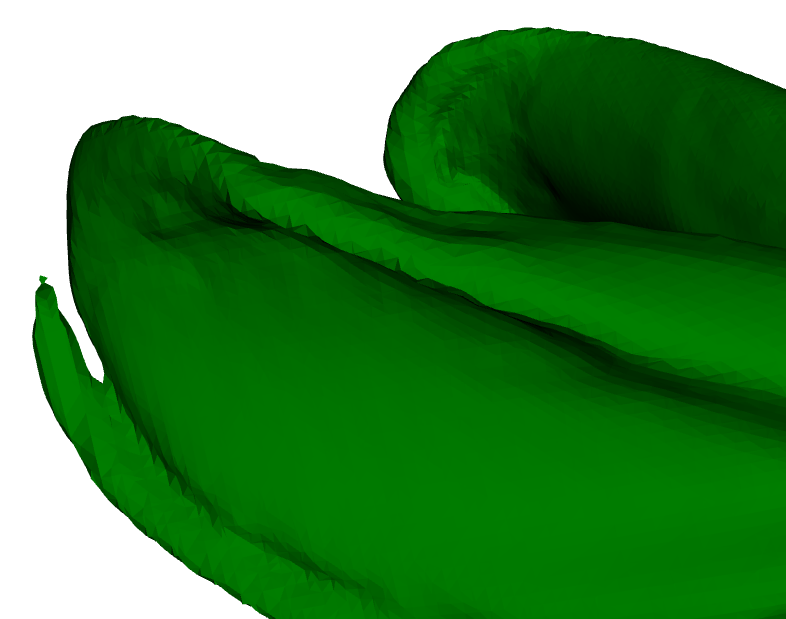
\includegraphics[max width=.5\linewidth, max height=.25\textheight, keepaspectratio]
				{img/bunny_ear}
			%\Imagen{img/bunny_ear}
			\caption{\label{fig:bun_ear}Acercamiento a la oreja derecha de bunny.}
		\end{figure}

		\begin{figure}
			%\Imagen{img/drill_drops}
			\centering
			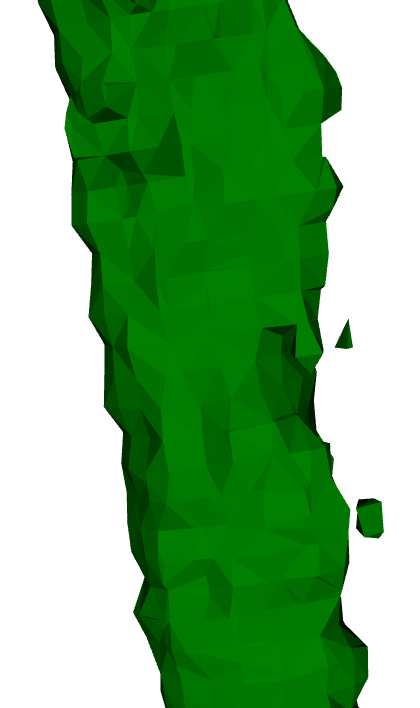
\includegraphics[max width=.5\linewidth, max height=.25\textheight, keepaspectratio]
				{img/drill_drops}
			\caption{\label{fig:drill_drops}Acercamiento a la mecha de drill. Se observan componentes inconexas con la malla principal.}
		\end{figure}

		\begin{figure}
			\centering
			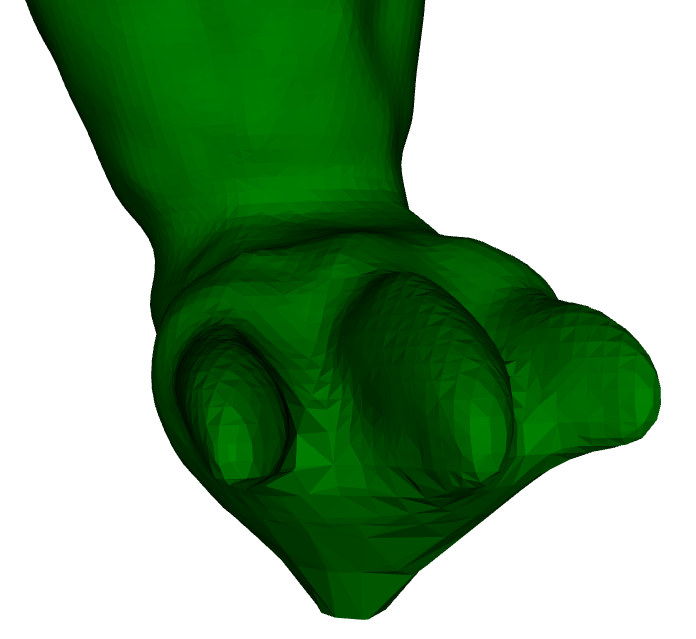
\includegraphics[max width=.5\linewidth, max height=.25\textheight, keepaspectratio]
				{img/arma_foot}
			%\Imagen{img/arma_foot}
			\caption{\label{fig:base}Acercamiento a la base de apoyo de armadillo. Se observa un estiramiento hacia abajo debido al uso de condiciones de borde Neumann.}
		\end{figure}



	\section{Conclusiones}
		Como resultado de esta etapa se obtuvo una biblioteca de software que
		permite reconstruir un objeto tridimensional a partir de nubes
		de puntos de vistas parciales sujetas a ciertas restricciones.
		Debido al uso del método de Poisson en el rellenado, esta
		reconstrucción no presentará huecos, a excepción de la base de apoyo.

		Durante la registración, se obtuvieron resultados aceptables en casi todas las pruebas, 
		siendo uno de los fallos debido a un ángulo excesivo entre las tomas.
		Estos fallos pueden detectarse al utilizar la métrica de solapamiento y entonces proceder
		a ajustar los parámetros del algoritmo de alineación.

		A futuro se pretende desarrollar algoritmos que nos permitan relajar la
		restricción del eje de giro.
		De esta forma, se podrán combinar reconstrucciones del mismo objeto
		sobre la base de giro, con lo que se logrará recuperar la información
		perdida debido a oclusiones.


	\chapter{Conclusiones y trabajos futuros}
\section{Del producto}
	En este proyecto se realizó el desarrollo de una biblioteca de software para
	realizar la reconstrucción tridimensional de un objeto a partir de capturas de
	vistas parciales.
	Para esto, se dividió el problema en tres módulos: registración, fusión y
	rellenado de huecos, y se implementaron diversos algoritmos.

	Al trabajar directamente con las nubes de puntos no se restringió el
	dispositivo de captura a un hardware en particular. Sin embargo, las
	restricciones impuestas de base giratoria y limitar la cantidad de capturas
	requeridas fueron planteadas considerando una integración futura con
	el trabajo realizado por \TODO{cite{Pancho}}.

	Las registraciones se obtuvieron en tiempos razonables, sin requerir hardware especial.
	Si bien se observa un efecto de «inflado» debido a la propagación de los errores de registración,
	este se encuentra suficientemente acotado respecto al tamaño del objeto.

	Al realizar las capturas solamente sobre una base giratoria,
	Debido a que las capturas se realizaron solamente sobre una base giratoria,
	no se lograron resolver todas las oclusiones, lo que genera la aparición de huecos de
	tamaño considerable.
	Aún así, el resultado es una malla cerrada, y la
	superficie estimada en las zonas sin información se une suavemente al resto de
	la malla.

\section{Del proceso}
La elección de la metodología en cascada modificada fue incorrecta.
La investigación bibliográfica se alargó demasiado y se desperdiciaron recursos
al abordar temas que tuvieron que ser descartados luego (como el uso de la
información de textura).
Además, se produjo un desfasaje entre la adquisición de los conocimientos y la
implementación de los mismos.

Hubiese sido mejor utilizar directamente una metodología incremental en todo el
proceso, con más incrementos de menor tamaño, como ser agregar un primer módulo
de preproceso que contenga la reducción de ruido y la operatoria básica con las
nubes de puntos.

En cuanto al desarrollo, uno de los principales problemas fue la definición de
métricas para evaluar los algoritmos y establecer qué niveles de error eran
aceptables y cuáles requerían una corrección.
Esto se dificulta, además, al considerar que los resultados producidos en una etapa
serán la entrada de otra, de la cual se desconoce su sensibilidad.
Muchas evaluaciones fueron primeramente visuales, resultando en un proceso lento
que en ocasiones fallaba en detectar errores considerables.



%\subsection{Riesgos efectivizados}
%Ausencia de repositorio de mallas tridimensionales
%(copiar base de datos)
%
%Falla en los equipos de trabajo
%(copiar parte de pcl)
%Meshlab: no se logró instalarlo en el nuevo equipo, se cambió a CloudCompare



\section{Trabajos futuros}
En esta sección se describirán actividades que excedieron el alcance de este proyecto
y podrían ser abordadas en una etapa posterior.

\begin{itemize}
	\item Combinar escaneos cilíndricos del objeto en varias posiciones sobre la base giratoria,
		buscando de esta forma eliminar huecos y reducir la propagación del error de alineación.
		Esto requerirá eliminar la restricción del eje de giro en la
		registración, por lo que deberán evaluarse otros métodos para detectar
		correspondencias erróneas.
	\item Ajustar los métodos para trabajar con el volumen de puntos generados
		por \TODO{cite{Pancho}}.  Las capturas de los modelos con los cuales se
		realizaron las pruebas contenían a lo sumo ochenta mil puntos. Las
		reconstrucciones obtenidas en \TODO{cite{Pancho}} pueden llegar a los
		dos millones, es decir, 25 veces más.
		Es necesario entonces, analizar la escalabilidad de los métodos
		propuestos y optimizarlos o reemplazarlos según resulte conveniente.
		En particular, puede plantearse la ejecución sobre GPU.
	\item Implementar métricas de calidad del mallado que consideren las
		características de la impresión 3D.
		En este proyecto solamente se consideraron las condiciones de que la malla
		resultase cerrada y no presente intersecciones consigo misma.
	%\item Mejorar la detección de \emph{outliers} en el módulo de fusión.
	%\item Implementar métodos de suavizado de mallas.
	\item Modificar el método de \emph{advancing front} para que utilice una
		superficie de soporte para establecer la posición de los nuevos puntos,
		asegurando de esta forma la convergencia del método y la suavidad del
		parche generado.
	\item Modificar el método de \emph{advancing front} para que considere las islas.
		Esto requerirá detectar dentro de qué hueco se encuentra cada isla.
\end{itemize}

	%Resumen
	%Introducción
	%   justificación
	%   objetivos
	%   requerimientos
	%Marco teórico
	%	Registración
	%		Keypoints
	%		Features
	%		ICP
	%	Fusión
	%		Mallado
	%	Rellenado y reconstrucción
	%		Poisson
	%		Advancing front
	%Desarrollo
	%	significado de los parámetros
	%Resultados
	%	calidad del mallado
	%	suavizado del mallado
	%	Ajustes para impresión 3D
	%	**Comparación contra otros métodos

	%Conclusiones y trabajos futuros
	%Bibliografía
	%\bibliographystyle{plainnat}
	\bibliographystyle{alpha}
	\bibliography{biblio}

	\appendix
	\chapter{Uso de la biblioteca}
En este apéndice se presenta una reseña de la biblioteca desarrollada.
Se explica brevemente la instalación, compilación y el uso de las funciones fundamentales
que provee cada módulo de la misma.

	\section{Instalación y compilación}
	La biblioteca se encuentra contenida en archivos de cabecera, los cuales serán incluidos por los fuentes del proyecto.
	Se requiere la instalación de las siguientes dependencias:
	\begin{itemize}
		\item \texttt{PCL} versión 1.9 (\url{https://pointclouds.org/downloads/}).
		\item \texttt{delaunator-cpp} versión 0.4 (\url{https://github.com/delfrrr/delaunator-cpp}).
		\item \texttt{DKM} (\url{https://github.com/genbattle/dkm}).
	\end{itemize}

	Para la compilación se recomienda el uso de la herramienta \texttt{cmake} con el siguiente esqueleto para su archivo de configuración \texttt{CMakeLists.txt}:
	\inputminted{cmake}{code/CMakeLists.txt}

	\section{Representación de las capturas}
		La clase \verb|cloud_with_transformation|
			agrupa la información de posición y normales de cada punto,
			y la transformación de alineación.
			Durante la registración, las posiciones y normales se mantienen en dos nubes separadas,
			sin embargo, los módulos de fusión y rellenado de huecos
			requieren esta información integrada en una sola nube.
			Para convertir a este segundo formato se provee la función 
			\mintinline{cpp}{join_cloud_and_normal(nube)}.
		%\item \verb|alignment|: realiza la registración de dos nubes mediante el método de búsqueda de clústeres.
		%\item \verb|fusion|: realiza la fusión de las nubes una vez alineadas.
		%\item \verb|advancing_front|: realiza el rellenado de los huecos mediante el algoritmo basado en advancing front.

	\section{Módulo de preproceso}
	\begin{itemize}
		\item Carga la nube desde un archivo de disco y la prepara para ser usada por el módulo de registración
	\inputminted{cpp}{code/preproceso.cpp}
	\end{itemize}

	\section{Módulo de registración}
	\begin{itemize}
		\item Alineación inicial de dos nubes
			\inputminted{cpp}{code/pairwise_reg.cpp}

		\item Ajuste mediante el algoritmo de ICP
			\inputminted{cpp}{code/pairwise_icp.cpp}

		\item Corrección de bucle.
			Se realiza sobre un vector que contiene todas las capturas realizadas alrededor del objecto.
			\inputminted{cpp}{code/loop.cpp}

		\item Medición de la calidad de la registración
			\inputminted{cpp}{code/fitness.cpp}
	\end{itemize}

	\section{Módulo de fusión}
	\begin{itemize}
		\item Fusión de las capturas alineadas y triangulación de la nube resultante
			\inputminted{cpp}{code/fusion.cpp}
	\end{itemize}

	\section{Rellenado de huecos}
	\begin{itemize}
		\item Detección de huecos
			\inputminted{cpp}{code/holes.cpp}

		\item Rellenado mediante el método de advancing front.
			\emph{¡Advertencia! El algoritmo falla excepto en huecos pequeños o planos.
			No se recomienda su uso}
			\inputminted{cpp}{code/adv_front.cpp}
	\end{itemize}

	\section{Reconstrucción de Poisson}
	\begin{itemize}
		\item Utilización del algoritmo de reconstrucción de Poisson implementado en la biblioteca PCL
			\inputminted{cpp}{code/poisson.cpp}
	\end{itemize}

\end{document}
